\documentclass{chezreport}
\usepackage{standalone}

\NewDocumentCommand{\blank}{}{\raisebox{0.4ex}{\texttt{\char32}}}
\NewDocumentCommand{\marksymb}{m}{\overset{\scalebox{0.6}{\ensuremath\bullet}}{#1}}

\NewDocumentCommand{\mapredu}{}{\mathrel{\leq_m}}
\NewDocumentCommand{\polyredu}{}{\mathrel{\leq_p}}
\NewDocumentCommand{\logredu}{}{\mathrel{\leq_L}}
\NewDocumentCommand{\HALT}{}{\mathit{HALT}}
\NewDocumentCommand{\REGEXup}{}{\textsf{REGEX}\mathord\uparrow}
\DeclareMathOperator{\TIME}{TIME}
\DeclareMathOperator{\SPACE}{SPACE}
\DeclareMathOperator{\NSPACE}{NSPACE}

\NewDocumentCommand{\numphi}{}{\textsf\#\phi}
\NewDocumentCommand{\hash}{}{\texttt\#}

\usetikzlibrary{automata, decorations.pathmorphing}
\tikzset{automaton/.style={->, shorten >=1pt, node distance=1.5cm, on grid,
                           auto, double distance=2pt,
                           every state/.style={minimum size=1.5em,
                           inner sep=1pt}}}

\title{18.404 Notes}
\author{Jason Chen \\ Lecturer: Michael Sipser}
\date{Last Updated: \today}

\begin{document}
\maketitle
\setcounter{tocdepth}{2}
\tableofcontents

% % Automata and Languages
% \documentclass{standalone}
\usepackage{chez}

\begin{document}
The class website is \href{https://math.mit.edu/~sipser/18404/}{\texttt{here}}.

\section{Finite Automata}
We're going to start with a discussion of computability, in which we need models of computation.

Let's start with an object \(M_1\) that is represented by the following diagram:
\begin{center}
	\begin{tikzpicture}[automaton, node distance=1.7cm]
		\node[state, initial]   (s_1) {\(q_1\)};
		\node[state]            (s_2) [right = of s_1] {\(q_2\)};
		\node[state, accepting] (s_3) [right = of s_2] {\(q_3\)};

		\path (s_1) edge [loop above] node {\(\texttt 0\)} (s_1);
		\path (s_1) edge [bend left]  node {\(\texttt 1\)} (s_2);
		\path (s_2) edge [bend left]  node {\(\texttt 0\)} (s_1);
		\path (s_2) edge []           node {\(\texttt 1\)} (s_3);
		\path (s_3) edge [loop right] node {\(\texttt 0, \texttt 1\)} (s_3);
	\end{tikzpicture}
\end{center}
We have the states \(q_1\), \(q_2\), and \(q_3\), transitions represented by the arrows and their labels, the start label labeled with an incoming arrow, and the accepting state with a double outline.

The inputs are strings, and to determine whether a string is accepted or rejected, we begin at the start input, and follow arrows corresponding to each character until reach the end of the string. If the ending state is an accepting state, we say that the input is accepted, and otherwise, the input is rejected.

\begin{example}
	In \(M_1\), \texttt{0101} is rejected and \texttt{01101} is accepted.
\end{example}

For a finite automata \(M\), we can think about all of the strings that \(M\) accepts:
\[
	\set{\text{strings \(w\)} \mid \text{\(M\) accepts \(w\)}}.
\]
We usually call this the language of \(M\), and we also sometimes say that \(M\) recognizes \(A\).

\subsection{More Rigorously}
\begin{definition}[Finite Automaton]
	A \vocab{finite automaton} \(M\) is a tuple \((Q, \Sigma, \delta, q_0, F)\) where
	\begin{itemize}[nosep]
		\item \(Q\) is a finite set of states,
		\item \(\Sigma\) is a set of symbols, called the \vocab{alphabet},
		\item \(\delta \colon Q \times \Sigma \to Q\) is the transition function, i.e. the arrows in the diagram,
		\item \(q_0 \in Q\) is the start state, and
		\item \(F \subseteq Q\) are the accepting states.
	\end{itemize}
\end{definition}

\begin{remark}
	Since \(\delta\) has a codomain of \(Q\), this is a deterministic finite automata, i.e. there is only one possible ``next'' output given a state and a symbol.
\end{remark}

\begin{definition}
	We say that a finite automaton \(M = (Q, \Sigma, \delta, q_0, F)\) \vocab{accepts} a string (a finite sequence of symbols in \(\Sigma\)) \(w = w_1 w_2 \dots w_n\), where \(w_i \in \Sigma\) if there exists a sequence of states \(r_0, r_1, \dots, r_n\) where
	\begin{itemize}[nosep]
		\item \(r_0 = q_0\),
		\item \(r_n \in F\), and
		\item \(\delta(r_{i - 1}, w_i) = r_i\) for \(1 \leq i \leq n\).
	\end{itemize}
\end{definition}

\begin{definition}
	The \vocab{language} of \(M\) is \(L(M) = \set{w \mid \text{$M$ accepts $w$}}\). Then, we say that \(M\) \vocab{recognizes} \(L(M)\).

	If \(A = L(M)\) for some finite automaton \(M\), then \(A\) is a \vocab{regular} language.
\end{definition}

\begin{example}[Regular Languages]
	\begin{itemize}[nosep]
		\item \(A = \set{w \mid \text{\texttt{11} is a substring of $w$}}\) is regular.
		\item \(B = \set{w \mid \text{$w$ starts and ends with the same symbol}}\) is regular.
		\item \(C = \set{w \mid \text{$w$ has an equal number of \texttt{0}s and \texttt{1}s}}\) is regular.
	\end{itemize}
\end{example}

\subsection{Operations}
We can also define operations on languages. Let \(A\) and \(B\) be languages. Then, the \vocab{union} of \(A\) and \(B\) is
\[
	A \union B = \set{w \mid \text{$w \in A$ or $w \in B$}}.
\]
The \vocab{concatenation} of \(A\) and \(B\) is
\[
	A \circ B = \set{xy \mid \text{$x \in A$ and $y \in B$}}.
\]
We will often omit the circle for convenience. The \vocab{star} operator gives
\[
	A^* = \set{x_1 x_2 \dots x_k \mid x_i \in A, k \in \NN}.
\]
Note that the empty string \(\eps\) is in \(A^*\) from the case \(k = 0\).

\begin{proposition}<union_of_regular_is_regular>
	If \(A\) and \(B\) are regular, then so is \(A \union B\).
\end{proposition}
\begin{proof}
	First we'll show that \(A \union B\) is regular. Suppose \(M_A = (Q_A, \Sigma, \delta_A, q_A, F_A)\) and \(M_B = (Q_B, \Sigma, \delta_B, q_B, F_B)\) recognize \(A\) and \(B\) respectively. We assume that the alphabets are the same, but the proof would be similar albeit messier if they were not the same. The idea is that we can ``run both of the machines at the same time''. In particular, we will keep track of the states of each machine in ordered pairs.

	Our desired finite automaton that accepts \(A \union B\) is \((Q, \Sigma, \delta, q, F)\), where
	\begin{itemize}[nosep]
		\item \(Q = Q_A \times Q_B\),
		\item \(\delta \colon ((a, b), \sigma) \mapsto (\delta_A(a, \sigma), \delta_B(b, \sigma))\),
		\item \(q = (q_A, q_B)\), and
		\item \(F = \set{(a, b) \in Q_A \times Q_B \mid \text{$a \in F_A$ or $b \in F_B$}} = (F_A \times Q_B) \union (Q_A \times F_B)\). \qedhere
	\end{itemize}
\end{proof}

\begin{remark}
	Note that we can prove that \(A \intersect B \coloneqq \set{w \mid \text{$w \in A$ and $w \in B$}}\) is regular with the exact same machine as \(A \union B\) except we replace the final states with \(F_A \times F_B\).
\end{remark}



\end{document}


% \documentclass{standalone}
\usepackage{chez}

\begin{document}
\section{More on Closure of Regular Operations}
\begin{proposition}<concat_of_regular_is_regular>
  If \(A\) and \(B\) are regular, then so is \(A \circ B\).
\end{proposition}
We can attempt to prove using the same method as
\cref{prop:union_of_regular_is_regular}.
Suppose that \(M_A = (Q_A, \Sigma, \delta_A, q_A, F_A)\) accepts \(A\) and
\(M_B = (Q_B, \Sigma, \delta_B, q_B, F_B)\) recognizes \(B\).
Then, intuitively, we want to run \(M_A\), and then run \(M_B\) on the input.
However, it's not clear how the new machine can decide when to split the input.

In particular, for a given \textsf{DFA} \(M\),
there is only one possible path that \(M\) will take for a specific input.
So \(M\) is not able to test all potential split points.

\section{Nondeterministic Finite Automata}
To fix this problem, let's allow the machine to make decisions.
\begin{center}
  \begin{tikzpicture}[automaton]
    \node[state, initial]     (q1) {\(q_1\)};
    \node[state, right=of q1] (q2) {\(q_2\)};
    \node[state, right=of q2] (q3) {\(q_3\)};
    \node[state, right=1.8cm of q3] (q4) {\(q_4\)};

    \path[loop above] (q1) edge node{\(\mathtt a, \mathtt b\)} (q1);
    \path             (q1) edge node{\(\mathtt a\)} (q2);
    \path             (q2) edge node{\(\mathtt b\)} (q3);
    \path             (q3) edge node{\(\mathtt a, \eps\)} (q4);
  \end{tikzpicture}
\end{center}
The idea is that at a particular state (e.g.\ \(q_1\)),
there may be multiple edges that the machine could take
(e.g.\ back to \(q_1\) or to \(q_2\) when the input is \(\mathtt a\)).
To think about a path that the machine takes while going through an input,
we keep track of a subset of the states that the machine could be at.
Moreover, if there exists an arrow exiting with an \(\eps\),
then we include both the current state as well as
the state that the \(\eps\) arrow goes to, as the machine can be at both.

\begin{example}
  In the machine described by the diagram above,
  \(\mathtt{ab}\) and \(\mathtt{aba}\) are accepted,
  while \(\mathtt{ba}\) and \(\mathtt{abaa}\) are rejected.
\end{example}

\begin{definition}
  A \vocab{nondeterministic finite automata} (\textsf{NFA}) is
  tuple \((Q, \Sigma, \delta, q_0, F)\) where
  \begin{itemize}[nosep]
    \item \(Q\) is a finite set of states,
    \item \(\Sigma\) is a finite alphabet,
    \item \(\delta \colon Q \times \Sigma_\eps \to \mathcal P(Q)\) is
          the transition function,
    \item \(q_0 \in Q\) is the start state, and
    \item \(F\) is the set of accepting states.
  \end{itemize}
  where \(\Sigma_\eps = \Sigma \union \set \eps\).
  Then, we say that the \textsf{NFA} \vocab{accepts} a string
  \(s = s_1 s_2 \dots s_n \in \Sigma^n\) if there exists
  a sequence of states \(r_0, \dots, r_n\) such that
  \begin{itemize}[nosep]
    \item \(r_0 = q_0\),
    \item \(r_n \in F\), and
    \item \(r_i \in \delta(r_{i - 1}, w_i)\) for \(1 \leq i \leq n\).
  \end{itemize}
\end{definition}

\begin{proposition}
  If \(N\) is a \textsf{NFA}, then \(L(N)\) is regular.
\end{proposition}
\begin{proof}
  Let \(N = (Q, \Sigma, \delta, q_0, F)\).
  We will show that there exists a \textsf{DFA} \(M\)
  that is equivalent to \(N\).
  The idea (again) is to keep track of the subset of
  the states that \(N\) can be at.
  Therefore, we let
  \begin{itemize}
    \item \(Q' = \mathcal P(Q)\),
    \item \(\delta' \colon (R, \sigma)
                    \mapsto \bigunion_{r \in R} \delta(r, \sigma)\),
    \item \(q_0' = \set{q_0}\), and
    \item \(F' = \set{q \in Q' \mid q \intersect F \neq \nullset}\).
  \end{itemize}
  The desired \textsf{DFA} is then \((Q', \Sigma, \delta', q_0', F')\).
\end{proof}
\begin{remark}
  We ignored \(\eps\) in this proof, but the idea is to consider
  \(E(R)\) for \(R \in Q'\) to be the set of states
  that can be reached by following \(\eps\) arrows, and then let
  \(\delta' \colon (R, \sigma)
            \mapsto E\parens{\bigunion_{r \in R} \delta(r, \sigma)}\).
\end{remark}

We can then write a new and better proof for one of our old propositions!
\begin{proof}[Closure of Regular Languages under \(\union\),
              \Cref{prop:union_of_regular_is_regular}]
  Suppose \(M_A = (Q_A, \Sigma, \delta_A, q_A, F_A)\) recognizes \(A\) and
          \(M_B = (Q_B, \Sigma, \delta_B, q_B, F_B)\) recognizes \(B\).
          Then consider the following machine:
  \begin{center}
    \begin{tikzpicture}[automaton]
      \node[state, initial] (q0) {};
      \node[state, above right=1.1cm and 1.7cm of q0] (q1) {\(q_A\)};
      \node[state, below right=1.1cm and 1.7cm of q0] (q2) {\(q_B\)};
      \node[state, accepting, above right=0.5cm and 1.7cm of q1] (q11) {};
      \node[state, accepting, below right=0.5cm and 1.7cm of q1] (q12) {};
      \node[state, accepting, above right=0.5cm and 1.7cm of q2] (q21) {};
      \node[state, accepting, below right=0.5cm and 1.7cm of q2] (q22) {};
      \node[right=0.8cm of q1] () {\(\cdots\)};
      \node[right=0.8cm of q2] () {\(\cdots\)};

      \node () at ($(q1) + (-0.3, 0.7)$) {\(M_A\)};
      \node () at ($(q2) + (-0.3, 0.7)$) {\(M_B\)};

      \draw[lightgray] ($(q1) + (-0.7, -1)$) rectangle ($(q11) + (0.7, 0.5)$);
      \draw[lightgray] ($(q2) + (-0.7, -1)$) rectangle ($(q21) + (0.7, 0.5)$);

      \path[bend left]  (q0) edge node{\(\eps\)} (q1);
      \path[bend right] (q0) edge node[swap]{\(\eps\)} (q2);
    \end{tikzpicture}
  \end{center}
  Note that this accepts factly the languages in \(A \union B\).
\end{proof}

\begin{proof}[\Cref{prop:concat_of_regular_is_regular}]
  Suppose \(M_A = (Q_A, \Sigma, \delta_A, q_A, F_A)\) recognizes \(A\) and
          \(M_B = (Q_B, \Sigma, \delta_B, q_B, F_B)\) recognizes \(B\).
          Then consider the following machine:
  \begin{center}
    \begin{tikzpicture}[automaton]
      \node[state, initial]                                      (q1) {\(q_A\)};
      \node[state, right=3.5cm of q1]                            (q2) {\(q_B\)};
      \node[state, above right=0.5cm and 1.7cm of q1] (q11)           {};
      \node[state, below right=0.5cm and 1.7cm of q1] (q12)           {};
      \node[state, accepting, above right=0.5cm and 1.7cm of q2] (q21) {};
      \node[state, accepting, below right=0.5cm and 1.7cm of q2] (q22) {};
      \node[right=0.8cm of q1] () {\(\cdots\)};
      \node[right=0.8cm of q2] () {\(\cdots\)};

      \node () at ($(q1) + (-0.3, 0.7)$) {\(M_A\)};
      \node () at ($(q2) + (-0.3, 0.7)$) {\(M_B\)};

      \draw[lightgray] ($(q1) + (-0.7, -1)$) rectangle ($(q11) + (0.7, 0.5)$);
      \draw[lightgray] ($(q2) + (-0.7, -1)$) rectangle ($(q21) + (0.7, 0.5)$);

      \path[bend left=10] (q11) edge node[pos=0.3]      {\(\eps\)} (q2);
      \path[bend right=10] (q12) edge node[pos=0.3, swap]{\(\eps\)} (q2);
    \end{tikzpicture}
  \end{center}
  This recognizes \(AB\).
\end{proof}

\begin{proposition}
  Let \(A\) be a regular language. Then \(A^*\) is regular.
\end{proposition}
\begin{proof}
  Let \(M = (Q, \Sigma, \delta, q_0, F)\) recognize \(A\).
  Then consider the following machine:
  \begin{center}
    \begin{tikzpicture}[automaton]
      \node[state, accepting, initial]                (q0)  {};
      \node[state, right=of q0]                       (q1)  {\(q_0\)};
      \node[state, accepting, above right=0.5cm and 1.7cm of q1] (q11) {};
      \node[state, accepting, below right=0.5cm and 1.7cm of q1] (q12) {};
      \node[right=0.8cm of q1] () {\(\cdots\)};

      \draw[lightgray] ($(q1) + (-0.5, -1)$) rectangle ($(q11) + (0.5, 0.5)$);

      \path (q0) edge node{\(\eps\)} (q1);
      \path[bend right=35] (q11) edge node[swap]{\(\eps\)} (q1);
      \path[bend left=35]  (q12) edge node{\(\eps\)}       (q1);
    \end{tikzpicture}
  \end{center}
  This accepts \(A^*\).
  Note that we did not make \(q_0\) accepting,
  but rather added a new start state.
  This is because within \(M\), there may be a sequence in \(A\)
  that ends on \(q_0\).
\end{proof}

\subsection{Regular Expressions}
Suppose we have an alphabet \(\Sigma\).
We want to find an easier way to describe languages.
In particular, we can use smaller languages to
build more complicated languages. We can use regular operations to do this.

A regular expression is an expression that uses
the regular operations that build on languages.
For example, we want something like
\((\mathtt{01} \union \mathtt 0)^*\) to be a regular expression.

\begin{definition}
  An expression \(R\) is a \vocab{regular expression} if either:
  \begin{itemize}
    \item \(R \in \Sigma \union \set{\eps, \nullset}\),
    \item \(R = R_1 \union R_2\) where \(R_1\) and \(R_2\) are languages,
    \item \(R = R_1 \circ R_2\) where \(R_1\) and \(R_2\) are languages, or
    \item \(R = R_0^*\) where \(R_0\) is a language.
  \end{itemize}
\end{definition}

Note that each of the atomic regular expressions represent languages:
\begin{itemize}
  \item \(a\) represents \(\set{a}\) for all \(a \in \Sigma\)
  \item \(\eps\) represents \(\set{\eps}\)
  \item \(\nullset\) represents \(\nullset\).
\end{itemize}
\begin{remark}
  The expressions \(\eps\) and \(\nullset\) do not represent the same language!
  \(\eps\) is the language that contains the empty string,
  and \(\nullset\) is the empty language.
\end{remark}

\begin{example}
  Consider the regular expression \(R = (\mathtt{01} \union \mathtt 0)^*\).
  We have \(\mathtt{01} \union \mathtt 0 \to \set{\mathtt{01}, \mathtt 0}\),
  so \(R\) represents the language
  \[
    \set{
      \eps,
      \mathtt{0},
      \mathtt{01},
      \mathtt{00},
      \mathtt{001},
      \mathtt{0100},
      \dots
    }.
  \]
  This is the language of all strings such that
  whenever a \(\mathtt 1\) appears, there is a \(\mathtt{0}\) before it.
\end{example}




\end{document}


% \documentclass{standalone}
\usepackage{chez}

\begin{document}
\section{More on Regular Expressions}
\begin{proposition}
  The set of languages that regular expressions determine is
  exactly all regular languages.
\end{proposition}
\begin{proof}[Regular expressions \(\implies\) regular]
  It is fairly clear that all regular expressions determine regular languages.
  In particular, for the atomic regular expressions,
  we can find the \textsf{NFA}s:
  \begin{itemize}
    \item \(a\) for \(a \in \Sigma_\eps\)
    \begin{center}
      \begin{tikzpicture}[automaton]
        \node[state, initial]                (q0) {};
        \node[state, accepting, right=of q0] (q1) {};
        \path (q0) edge node{\(a\)} (q1);
      \end{tikzpicture}
    \end{center}

    \item \(\nullset\)
    \begin{center}
      \begin{tikzpicture}[automaton]
        \node[state, initial] (q0) {};
      \end{tikzpicture}
    \end{center}
  \end{itemize}

  For the composite regular expressions,
  we just can use the regular operations for \textsf{NFA}s.
\end{proof}

\begin{example}
  If we want to build an \textsf{NFA} for \((\mathtt a \union \mathtt{ab})^*\),
  we can just build it up from smaller parts:
  \begin{itemize}[nosep]
    \item \(\mathtt a\)
    \begin{center}
      \begin{tikzpicture}[automaton]
        \node[state, initial]                (q0) {};
        \node[state, accepting, right=of q0] (q1) {};
        \path (q0) edge node{\(\mathtt a\)} (q1);
      \end{tikzpicture}
    \end{center}

    \item \(\mathtt b\)
    \begin{center}
      \begin{tikzpicture}[automaton]
        \node[state, initial]                (q0) {};
        \node[state, accepting, right=of q0] (q1) {};
        \path (q0) edge node{\(\mathtt b\)} (q1);
      \end{tikzpicture}
    \end{center}

    \item \(\mathtt{ab}\)
    \begin{center}
      \begin{tikzpicture}[automaton]
        \node[state, initial]                (q0) {};
        \node[state, right=of q0]            (q1) {};
        \node[state, right=of q1]            (q2) {};
        \node[state, accepting, right=of q2] (q3) {};
        \path (q0) edge node{\(\mathtt a\)} (q1);
        \path (q1) edge node{\(\eps\)} (q2);
        \path (q2) edge node{\(\mathtt b\)} (q3);
      \end{tikzpicture}
    \end{center}

    \item \(\mathtt a \union \mathtt{ab}\)
    \begin{center}
      \begin{tikzpicture}[automaton]
        \node[state, initial]                (qn1) {};
        \node[state, below right=0.6cm and 1cm of qn1]     (q0) {};
        \node[state, right=of q0]            (q1) {};
        \node[state, right=of q1]            (q2) {};
        \node[state, accepting, right=of q2] (q3) {};
        \node[state, above right=0.6cm and 1cm of qn1]     (q4) {};
        \node[state, accepting, right=of q4] (q5) {};
        \path (qn1) edge node[swap]{\(\mathtt \eps\)} (q0);
        \path (qn1) edge node{\(\mathtt \eps\)} (q4);
        \path (q0) edge node{\(\mathtt a\)} (q1);
        \path (q1) edge node{\(\eps\)} (q2);
        \path (q2) edge node{\(\mathtt b\)} (q3);
        \path (q4) edge node{\(\mathtt a\)} (q5);
      \end{tikzpicture}
    \end{center}

    \item \((\mathtt a \union \mathtt{ab})^*\)
    \begin{center}
      \begin{tikzpicture}[automaton]
        \node[state, initial, accepting]     (qn2) {};
        \node[state, right=of qn2]           (qn1) {};
        \node[state, below right=0.6cm and 1cm of qn1]     (q0) {};
        \node[state, right=of q0]            (q1) {};
        \node[state, right=of q1]            (q2) {};
        \node[state, accepting, right=of q2] (q3) {};
        \node[state, above right=0.6cm and 1cm of qn1]     (q4) {};
        \node[state, accepting, right=of q4] (q5) {};

        \path (qn2) edge node{\(\mathtt \eps\)} (qn1);
        \path (qn1) edge node[swap]{\(\mathtt \eps\)} (q0);
        \path (qn1) edge node{\(\mathtt \eps\)} (q4);
        \path (q0) edge node{\(\mathtt a\)} (q1);
        \path (q1) edge node{\(\eps\)} (q2);
        \path (q2) edge node{\(\mathtt b\)} (q3);
        \path (q4) edge node{\(\mathtt a\)} (q5);
        \path[bend right=45] (q5) edge node[swap]{\(\eps\)} (qn2);
        \path[bend left=30] (q3) edge node{\(\eps\)} (qn2);
      \end{tikzpicture}
    \end{center}
  \end{itemize}
\end{example}

To prove that all \textsf{NFA}s can be represented by a regular expression,
we will define another version of them that will make things more convenient.
\begin{definition}
  A \vocab{generalized nondeterministic finite automaton (\textsf{GNFA})}
  is an \textsf{NFA} that can have regular expressions as transition labels.
\end{definition}

\begin{example}
  This is a \textsf{GNFA}, and it accepts \(\mathtt{abbbabab}\):
  \begin{center}
    \begin{tikzpicture}[automaton, node distance=2cm]
      \node[state, initial] (q0) {};
      \node[state, right=of q0] (q1) {};
      \node[state, accepting, below right=of q0] (q2) {};

      \path (q0) edge node{\(\mathtt{ab}^*\)} (q1);
      \path[loop above] (q1) edge node{\(\mathtt{bb}\)} (q1);
      \path (q0) edge node[swap]{\(\eps\)} (q2);
      \path (q1) edge node[pos=0.3]{\((\mathtt a \union \mathtt{ab})^*\)} (q2);
    \end{tikzpicture}
  \end{center}
\end{example}

\begin{proof}[\textsf{GNFA} \(\implies\) regex]
  Suppose we have a \textsf{GNFA}.
  For convenience, assume that the starting state is not accepting.
  (We can just add another starting state with an \(\eps\) arrow
  pointing to it otherwise.)
  Also, assume that there are only arrows out of the initial state,
  and there are only arrows going into a single accepting state.
  We can ensure this by adding \(\eps\) arrows.

  We proceed by induction.
  The smallest machine that satisfies these conditions
  is one that has \(k = 2\) states, and it looks like this
  \begin{center}
    \begin{tikzpicture}[automaton]
      \node[state, initial] (q0) {};
      \node[state, accepting, right=of q0] (q1) {};
      \path (q0) edge node{\(r\)} (q1);
    \end{tikzpicture}
  \end{center}
  where \(r\) is some regular expression.
  This is the regular expression for this \textsf{GNFA}.

    Now suppose that all \textsf{GNFA}s with at most \((k-1)\) states
    has an equivalent regular expression.
    Consider some \textsf{GNFA} \(G\) with \(k\) states.
    Our goal is to make a new \textsf{GNFA} with \(k - 1\) states.
    Let's remove some state \(g_x\).
    For all states \(q_i, q_j \neq g_x\) in \(G\),
    we an make the following change to fix the machine:
  \begin{center}
    \begin{tikzpicture}[automaton]
      \node[state] (qi) {\(q_i\)};
      \node[state, right=2cm of qi] (qj) {\(q_j\)};
      \node[state] (qx) at ($(qi)!0.5!(qj) + (0, 1.4)$) {\(q_x\)};

      \path (qi) edge node{\(r_1\)} (qx);
      \path[loop above] (qx) edge node{\(r_2\)} (qx);
      \path (qx) edge node{\(r_3\)} (qj);
      \path (qi) edge node[swap]{\(r_4\)} (qj);

      \draw[lightgray] ($(qi) + (-0.6, -0.6)$) rectangle ($(qx) + (1.6, 1.3)$);
      
      \node (arr) at ($(qx) + (2.4, -0.3)$) {\(\implies\)};

      \node[state] (qip) at ($(arr) + (1.4, 0)$) {\(q_i\)};
      \node[state, right=3cm of qip] (qjp) {\(q_j\)};
      \path (qip) edge node{\(r_1 (r_2)^* r_3 \union r_4\)} (qjp);
      \draw[lightgray] ($(qip) + (-0.6, -0.6)$) rectangle ($(qjp) + (0.6, 0.7)$);
    \end{tikzpicture}
  \end{center}
  This gives a machine with \(k - 1\) states,
  and it accepts the same language, as desired.
\end{proof}

\section{Non-regularity}
Let \(B = \set{w \mid \text{$w$ has an equal number of
                            $\mathtt a$s and $\mathtt b$s}}\) and
    \(C = \set{w \mid \text{$w$ has an equal number of
                            $\mathtt{ab}$s and $\mathtt{ba}$s substrings}}\).
It turns out that \(B\) is not regular but \(C\) is regular.
It's not obviously clear how to determine this,
so it would be nice to have a method to determine
whether a language is regular or not.

\begin{proposition}[Pumping Lemma]
If \(A\) is a regular language, there exists some \(p \in \NN\) called
the \vocab{pumping length} such that if \(s \in A\) with \(\size s \geq p\),
we can write \(s = xyz\) where
\begin{itemize}[nosep]
\item \(xy^i z \in A\) for \(i \in \set{0, 1, 2, \dots}\),
\item \(y \neq \eps\), and
\item \(\size{xy} \leq p\).
\end{itemize}
\end{proposition}
\begin{proof}
  Let \(M\) be a \textsf{DFA} for a regular language \(A\),
  and let \(p\) be the number of states of \(M\).
  Let \(s \in A\) have length \(\size s \geq p\).
  
  Consider the states that the machine will visit
  while going through the string.
  Since \(\size s \geq p\), the machine will visit at least \(p + 1\) states.
  By the pigeonhole principle, the machine will visit
  some state \(q\) at least twice.
  \begin{center}
    \begin{tikzpicture}[automaton,
                        decoration={snake, amplitude=0.5mm, post length=1mm}]
      \node[state, initial] (q0) {};
      \node[state, above right=of q0] (q1) {\(q\)};
      \node[state, accepting, below right=of q1] (q2) {};
      
      \path (q0) edge[decorate] node{\(x\)} (q1);
      \path (q1) edge[decorate] node{\(y\)} (q2);
      \path (q1) edge[decorate, in=40, out=140, looseness=20]
                 node[above=0.1]{\(z\)} (q1);
    \end{tikzpicture}
  \end{center}
  Then, that means there is a nonempty string \(y\) that transitions
  from state \(q\) to \(q\), so we can repeat is as many times as possible.
\end{proof}

We can now use the pumping lemma to prove things!
\begin{claim}
  Let \(D = \set{\mathtt a^k \mathtt b^k \mid k \in \NN}\).
  Then \(D\) is not regular.
\end{claim}
\begin{proof}
  Assume for the sake of contradiction that \(D\) is regular.
  Then let the pumping length be \(p\), and consider
  \(s = \mathtt a^p \mathtt b^p \in D\).
  By the pumping lemma, we can write \(s = xyz\)
  where \(y = \mathtt a^n\) for some \(n > 0\).
  Then, this gives \(\mathtt a^{p + kn}\mathtt b^{p} \in D\)
  for all \(k \in \set{0, 1, \dots}\), which is a contradiction.
\end{proof}




\end{document}

% \documentclass{standalone}
\usepackage{chez}

\begin{document}
\section{Context-Free Grammars}
We will introduce a stronger model of computation.
\begin{example}
	Consider a set of substitution rules like the following:
	\begin{align*}
		S &\to \mathtt 0 S \mathtt 1 \\
		S &\to R \\
		R &\to \eps
	\end{align*}
	We have capital letters designating variables, and numbers or lowercase letters designating terminals. Start with the starting variable (usually the first one in the first line), and then make substitutions according to the rules.

	For instance, we can have
	\[
		S
			\to \mathtt 0 S \mathtt 1
			\to \mathtt 0 \mathtt 0 S \mathtt 1 \mathtt 1
			\to \mathtt 0 \mathtt 0 \eps \mathtt 1 \mathtt 1 = \mathtt{0011}
	\]

	Then, the language that this grammar \(G_1\) describes is \(L(G_1) = \set{\mathtt 0^k \mathtt 1^k \mid k \geq 0}.\)
\end{example}

\begin{example}
	Consider the grammar
	\begin{align*}
		E &\to E + T \mid T \\
		T &\to T \times F \mid T \\
		F &\to \texttt ( e \texttt ) \mid \mathtt a,
	\end{align*}
	where the variables are \(\set{E, T, F}\) and the terminals are \(\set{\texttt (, \texttt ), +, \times, \mathtt a}\).

	One string that this grammar can generate is
	\[
		E
			\to E + T
			\to T + T
			\to T + T \times F
			\to F + F \times \mathtt a
			\to \mathtt a + \mathtt a \times \mathtt a.
	\]
\end{example}

\begin{definition}
	A \vocab{context-free grammar (CFG)} is \(G = (V, \Sigma, R, S)\) where
	\begin{itemize}[nosep]
		\item \(V\) is a finite set of variables,
		\item \(\Sigma\) is a finite set of terminals
		\item \(R\) is a finite set of rules, and
		\item \(S \in V\) is a start variable.
	\end{itemize}

	If \(u, v, w\) are strings of variables and terminals and \(A \to w\) is a rule, we write \(uAv \Rightarrow uwv\) (read \(uAv\) \vocab{yields} \(uwv\)). In particular, \(u \Rightarrow v\) if we can get from \(u\) to \(v\) with one substitution.

	We also write \(u \overset{*}{\Rightarrow} v\) (read \(u\) \vocab{derives} \(v\)) if there exists a chain
	\[
		u \Rightarrow u_1 \Rightarrow u_2 \Rightarrow \dots \Rightarrow v.
	\]

	Then, the \vocab{language} of a grammar \(G\) is
	\[
		L(G) = \set{w \mid S \overset{*}{\Rightarrow} w}.
	\]
\end{definition}

\section{Pushdown Automata}
Context-free grammars for context-free languages are similar to regular expressions for regular languages in the sense that they both generate strings in the language. \textsf{DFA}s and \textsf{NFA}s work in the opposite way, i.e. they recognize strings in the language.

We'll introduce a machine that can recognize context-free languages in the same way that \textsf{DFA}s and \textsf{NFA}s recognize regular languages.

The idea is that there is a state control, which contains the states and transitions that we are familiar with. In addition to reading the input, the states can also control a stack, which is an object that has an infinite amount of memory to store things. The catch is that the machine can only read and write to the top of the stack.
\begin{center}
	\begin{tikzpicture}
		\node[rectangle]                         (sc) [draw] {state control};
		\node[right=1.8cm of sc]                 (input) {};
		\node[below right=2cm and 0.6cm of sc] (stack) {};

		\draw (input) rectangle ($(input) + (3, 0.6)$);
		\draw ($(input) + (0.6, 0)$) -- ($(input) + (0.6, 0.6)$);
		\draw ($(input) + (1.2, 0)$) -- ($(input) + (1.2, 0.6)$);
		\path ($(input) + (1.5, 0.6)$) node[above] {input};
		\path[->, bend left, shorten >=2pt] (sc.east) edge ($(input) + (0, 0.6)$);

		\draw (stack) rectangle ($(stack) + (0.6, 1.8)$);
		\draw[shorten >=0pt] ($(stack) + (0, 0.6)$) -- ($(stack) + (0.6, 0.6)$);
		\draw[shorten >=0pt] ($(stack) + (0, 1.2)$) -- ($(stack) + (0.6, 1.2)$);
		\path ($(stack) + (0.6, 0.9)$) node[right] {stack};
		\path ($(stack) + (0.3, 0)$) node[below] {\(\vdots\)};
		\path[->, bend left=20, shorten >=2pt] (sc.east) edge ($(stack) + (0.3, 1.8)$);
	\end{tikzpicture}
\end{center}

\begin{example}
	There exists a \textsf{PDA} that recognizes \(\set{\mathtt 0^k \mathtt 1^k}\).

	\tcblower
	Consider the \textsf{PDA} that pushes a \(\mathtt 0\) onto the stack when it reads a \(\mathtt 0\) at the beginning, and pops a \(\mathtt 0\) from the stack when it reads a \(\mathtt 1\) after the string of \(\mathtt 0\)s. This accepts \(\set{\mathtt 0^k \mathtt 1^k}\).
	\begin{center}
		\begin{tikzpicture}[automaton, node distance=2.2cm]
			\node[state, initial]                (q0) {};
			\node[state, right=of q0]            (q1) {};
			\node[state, right=of q1]            (q2) {};
			\node[state, accepting, right=of q2] (q3) {};

			\path (q0) edge node{\(\eps, \eps \to \texttt \$\)} (q1);
			\path[loop above] (q1) edge node{\(\mathtt 0, \eps \to \mathtt 0\)} (q1);
			\path (q1) edge node{\(\eps, \eps \to \eps\)} (q2);
			\path[loop above] (q2) edge node{\(\mathtt 1, \mathtt 0 \to \eps\)} (q2);
			\path (q2) edge node{\(\eps, \texttt \$ \to \eps\)} (q3);
		\end{tikzpicture}
	\end{center}
\end{example}


\begin{definition}
	A \vocab{pushdown automata (\textsf{PDA})} is \(M = (Q, \Sigma, \Gamma, \delta, q_0, F)\) where
	\begin{itemize}[nosep]
		\item \(Q\) is finite set of states,
		\item \(\Sigma\) is a finite input alphabet,
		\item \(\Gamma\) is a finite stack alphabet,
		\item \(\delta \colon Q \times \Sigma_\eps \times \Gamma_\eps \to \mathcal P(Q \times \Gamma_\eps)\) is the transition function,
		\item \(q_0 \in Q\) is the start state, and
		\item \(F \subseteq Q\) is the set of accepting states.
	\end{itemize}
\end{definition}

Then, we say that the pushdown automata \(M = (Q, \Sigma, \Gamma, \delta, q_0, F)\) accepts some input \(w = w_1 w_2 \dots w_n \in \Sigma^n\) if there exists a sequence of states \(r_0, \dots, r_n\) and a sequence of strings \(s_0, \dots, s_n \in \Gamma^*\) such that
\begin{itemize}
	\item \(r_0 = q_0\),
	\item \(s_0 = \eps\),
	\item \(r_n \in F\),
	\item \((q_i, b) \in \delta(q_{i - 1}, w_i, a)\), \(s_{j - 1} = at\), and \(s_j = bt\) for some \(a, b \in \Gamma_\eps\) and \(t \in \Gamma_\eps^*\) for \(1 \leq i \leq n\), and
	\item \(r_n \in F\).
\end{itemize}

\begin{example}
	There exists a \textsf{PDA} that recognizes \(B = \set{w w^R \mid w \in \set{\mathtt 0, \mathtt 1}^*},\) where \(w^R\) is the reverse of \(w\).

	\tcblower
	Let \(\Gamma = \Sigma\), and let the \textsf{PDA} push the read characters into the stack. Then at an arbitrary time, the \textsf{PDA} starts popping the read characters from the stack. By nondeterminism, this should work.

	\begin{center}
		\begin{tikzpicture}[automaton, node distance=2.2cm]
			\node[state, initial]                (q0) {};
			\node[state, right=of q0]            (q1) {};
			\node[state, right=of q1]            (q2) {};
			\node[state, accepting, right=of q2] (q3) {};

			\path (q0) edge node{\(\eps, \eps \to \texttt \$\)} (q1);
			\path[loop above] (q1) edge node{\(a, \eps \to a\)} (q1);
			\path (q1) edge node{\(\eps, \eps \to \eps\)} (q2);
			\path[loop above] (q2) edge node{\(a, a \to \eps\)} (q2);
			\path (q2) edge node{\(\eps, \texttt \$ \to \eps\)} (q3);
		\end{tikzpicture}
	\end{center}

	The reason why we push a \(\texttt \$\) onto the stack at the beginning is so that the machine has a way to tell if it is at the bottom of the stack. This is a common idea that will appear often.
\end{example}

\end{document}


% \documentclass{standalone}
\usepackage{chez}

\begin{document}
\section{CFGs and PDAs}
\begin{proposition}
  A language \(A\) is a \textsf{CFL} if and only if \(A = L(P)\)
  for some pushdown automata \(P\).
\end{proposition}
\begin{proof}[\(\textsf{CFG} \to \textsf{PDA}\)]
  The idea is that we can simulate a \textsf{CFG} using the stack
  to remember the intermediate strings.
  Initially, we insert the starting variable in the stack,
  and then when we see a variable at the top of a stack,
  we can replace it with any of the variable's rules.
  When we see a terminal at the top of the stack,
  we compare it with the input.
  If the \textsf{CFG} can generate the string,
  then eventually, we will remove everything in the stack.
  Overall, we have the following \textsf{PDA}:
  \begin{center}
    \begin{tikzpicture}[automaton, node distance=1.3cm]
      \node[state, initial]                (q0) {};
      \node[state, below=of q0]            (q1) {};
      \node[state, accepting, below=of q1] (q2) {};
      
      \path (q0) edge node{\(\eps, \eps \to \texttt \$ S\)} (q1);
      \path[loop right] (q1) edge
        node{\(\eps, \text{$A \to A'$ for all rules $A \to A'$}\)} (q1);
      \path[loop left] (q1) edge node{\(a, a \to \eps\)} (q1);
      \path (q1) edge node{\(\eps, \texttt \$ \to \eps\)} (q2);
    \end{tikzpicture}
  \end{center}
\end{proof}

\begin{proposition}[Pumping Lemma for \textsf{CFL}s]
  Given a \textsf{CFL} \(A\), there exists a \vocab{pumping length} \(p\)
  such that for all \(s \in A\) where \(\size s > p\),
  we can write \(s = uvxyz\) such that
  \begin{itemize}[nosep]
    \item \(uv^i x y^i z \in A\) for all \(i \in \set{0, 1, \dots}\),
    \item \(\size{vy} > 0\), and
    \item \(\size{vxy} \leq p\).
  \end{itemize}
\end{proposition}
\begin{proof}
  The idea is that given a \textsf{CFG} \(G\),
  there is some maximum rule length, so given some final string length,
  we can find a lower bound for the parse tree height.
  Therefore, for a sufficiently large final string length,
  we have a sufficiently tall parse tree.
  
  \begin{center}
    \begin{tikzpicture}[scale=0.9]
      \node[inner sep=0.15em] (R) at (0, 0) {\(R\)};
      \draw (R) -- +(2, -2)
        +(-2, -2) -- (R);

      \node[inner sep=0.15em] (R2) at (0.1, -1) {\(R\)};
      \draw (R2) -- +(1, -1)
        +(-1, -1) -- (R2);

      \draw ($(R) + (-2, -2)$) -- node[below]{\(v\)} ($(R2) + (-1, -1)$);
      \draw ($(R2) + (-1, -1)$) -- node[below]{\(x\)} ($(R2) + (1, -1)$);
      \draw ($(R2) + (1, -1)$) -- node[below]{\(y\)} ($(R) + (2, -2)$);

      \node[below right=0.7 and 2 of R] (arr) {\(\to\)};

      \node[inner sep=0.15em, above right=0.7 and 2 of arr] (R3) {\(R\)};
      \draw (R3) -- +(2, -2)
        +(-2, -2) -- (R3);

      \node[inner sep=0.15em] (R4) at ($(R3) + (0.1, -1)$) {\(R\)};
      \draw (R4) -- +(2, -2)
        +(-2, -2) -- (R4);
      \draw ($(R3) + (-2, -2)$) -- node[below]{\(v\)} ($(R4) + (-1, -1)$);
      \draw ($(R4) + (1, -1)$) -- node[below]{\(y\)} ($(R3) + (2, -2)$);

      \draw ($(R4) + (-2, -2)$) -- node[below]{\(vxy\)} ($(R4) + (2, -2)$);
    \end{tikzpicture}
  \end{center}

  If \(n = \size V\) is the number of variables,
  then consider a path from the initial variable to some terminal
  that has more than \(n\) variables.
  By pigeonhole, there exists some variable \(R\) that occurs more than once.
  Let the final result of the later \(R\) be \(x\),
  and the earlier \(R\) be \(vxy\).
  Then we can replace the later \(R\) with \(vxy\),
  and using a similar strategy,
  we can replace the earlier \(R\) with any \(v^i x y^i\).

  More formally, if \(b\) is the longest length
  of the right sides of all rules, then for a tree of height \(h\),
  the string length \(s\) satisfies \(s \leq b^h\).
  This means if we let \(p = b^{\size V + 1}\),
  we must have \(h \geq \size V + 1\),
  and there must be some repeated variable.

  Another thing we might need to worry about is
  if we have some rules of the form
  \[
    R \to S \to \dots \to R.
  \]
  To fix this, we can just say that given some string \(s \in A\),
  we will take the shortest parse tree for \(s\),
  i.e.\ we don't waste any time with rules that don't do anything.
\end{proof}

\begin{corollary}
  The language \(B = \set{\mathtt a^k \mathtt b^k \mathtt c^k}\)
  is not a \textsf{CFL}.
\end{corollary}
\begin{proof}
  For the sake of contradiction suppose \(B\) is regular.
  Then consider \(s = \mathtt a^p \mathtt b^p \mathtt c^p \in B\),
  where \(p\) is the pumping length.
  By the pumping lemma, we can write
  \(\mathtt a^p \mathtt b^p \mathtt c^p = uvxyz\)
  such that \(\size{vxy} \leq p\).
  In particular, this means that \(v\) and \(y\)
  can only contain two distinct letters.
  Therefore the pumping lemma states that \(uxz \in B\).
  However, we know that at least one of the number of \(\mathtt a\)s,
  \(\mathtt b\)s, and \(\mathtt c\)s must have changed,
  but not all of them, which is a contradiction.
\end{proof}

\begin{corollary}
  The language \(C = \set{ww \mid w \in \set{\mathtt a, \mathtt b}^*}\)
  is not context free.
\end{corollary}
\begin{proof}
  For the sake of contradiction, suppose that \(C\) is regular.
  Then consider \(s = \mathtt a^p \mathtt b^p \mathtt a^p \mathtt b^p \in C\),
  where \(p\) is the pumping length.
  By the pumping lemma, we can write \(s = uvwxy\) where \(\size{vwy} \leq p\).
  Therefore, \(vwy\) cannot contain \(\mathtt a\)s from both strings,
  and also cannot contain \(\mathtt b\)s from both strings.
  Therefore, when we pump, we will be changing the number of \(\mathtt a\)s
  (or \(\mathtt b\)s) in one of the \(w\)s but not the other.
\end{proof}

\chapter{Computability Theory}
\section{Turing Machines}
We would like a model of model of computation that is stronger than this.
In particular, it will be similar to a pushdown automata,
except instead of a stack, the machine reads and writes to
an unbounded tape that initially contains the input,
that it can move left and right on,
and it accepts/rejects by entering special halting states.

\begin{example}
  Recall the language \(B = \set{\mathtt a^k \mathtt b^k \mathtt c^k}\).
  We claim that there is a Turing machine for \(B\).

  \tcblower
  The idea is that on the first pass (staring from the leftmost position),
  the machine tests to make sure that the input is of the form
  \(\mathtt a^* \mathtt b^* \mathtt c^*\).
  Then, after that we can make multiple passes,
  each one replacing one \(\mathtt a\), one \(\mathtt b\),
  and one \(\mathtt c\) with a blank space each time.
\end{example}

\begin{definition}
  A \vocab{Turing machine (\textsf{TM})} is a tuple
  \((Q, \Sigma, \Gamma, \delta, q_0, q_{\text{acc}}, q_{\text{reg}})\)
  such that
  \begin{itemize}[nosep]
    \item \(Q\) is the set of states,
    \item \(\Sigma\) is the input alphabet not containing \blank,
    \item \(\Gamma\) is the tape alphabet with
          \(\blank \in \Gamma\) and \(\Sigma \subseteq \Gamma\),
    \item \(\delta \colon Q \times \Gamma \to
                          Q \times \Gamma \times \set{\mathrm L, \mathrm R}\)
          is the transition function,
    \item \(q_0 \in Q\) is the start state,
    \item \(q_{\text{accept}} \in Q\) is the accept state, and
    \item \(q_{\text{reject}} \in Q\) is the reject state,
          where \(q_{\text{accept}} \neq q_{\text{reject}}\).
  \end{itemize}
\end{definition}

The Turing machine begins its computation with the input on
the leftmost part of the tape, and the rest of the tape is filled with \blank.
The read/write head starts on the leftmost space of the tape.

As the Turing machine computes, the state,
tape contents, and head location changes.
A combination of these three items is a
\vocab{configuration} of the Turing machine.
We represent them in a specific way.
If the current state is \(q\), the tape contains \(uv \in \Gamma^*\),
and the tape head is on the first character of \(v\),
then we say that the configuration is \(uqv\).

We will say that a configuration \(C_1\) yields \(C_2\) if the Turing machine
can go from \(C_1\) to \(C_2\) in one step.
More formally, for all \(u, v \in \Gamma^*\),
if for some \(a, b, c \in \Gamma\)
we have \(\delta(q_i, b) = (q_j, c, \mathrm L)\), then
\[
  ua q_i bv \quad\text{yields}\quad u q_i acv,
\]
and if \(\delta(q_i, b) = (q_j, c, \mathrm R)\), then
\[
  ua q_i bv \quad\text{yields}\quad uac q_j v.
\]
If the head is at the left end, then receiving an \(\mathrm L\)
will not move the head.

The \vocab{starting configuration} of \(M\) on input \(w\)
is the configuration \(q_0 w\).
An \vocab{accepting configuration} is one where
the state is \(q_{\text{accept}}\),
and a \vocab{rejecting configuration} is one where
the state is \(q_{\text{reject}}\).
We call accepting and rejecting configurations \vocab{halting configurations},
and do not yield any configurations.
If the machine never halts, then we say that it \vocab{loops}.

Then, we say that \(M\) accepts a string \(w\) if
there exists configurations \(C_1, \dots, C_k\) such that \(C_1 = q_0 w\),
\(C_i\) yields \(C_{i + 1}\), and \(C_k\) is an accepting configuration.
Then the \vocab{language of \(M\)} is
\[
  L(M) \coloneqq \set{w \in \Sigma^* \mid \text{$M$ accepts $w$}}.
\]
We also say that \(M\) \vocab{recognizes} \(L(M)\).





\end{document}



% Computability Theory
% \documentclass{standalone}
\usepackage{chez}

\begin{document}
\begin{definition}
	A language \(L\) is \vocab{Turing-recognizable} if there exists
  some Turing machine \(M\) such that \(L = L(M)\).

	\tcblower
	A machine \(M\) is a \vocab{decider} if it always halts on all inputs.
  We then say that \(M\) \vocab{decides} \(L(M)\).

	Moreover, a language \(L\) is \vocab{Turing-decidable} if
  there exists some Turing machine that decides \(L\).
\end{definition}

\section{Variants of Turing Machines}
\begin{definition}
	A \vocab{multitape Turing machine} is the same as a Turing machine,
  but there are some finite number \(k\) of tapes,
  and the transition function is
	\[
		\delta \colon Q \times \Gamma^k \to
                  Q \times \Gamma^k \times \set{\mathrm L, \mathrm R}^k.
	\]
	The input is initially on the first string, while the others are blank.
\end{definition}

\begin{proposition}
	A language \(A\) is \(L(M)\) for some multitape \textsf{TM} \(M\)
  if and only if \(A\) is Turing-recognizable.
\end{proposition}
\begin{proof}
	The proof of the reverse direction is immediate.
	
	To prove the forward direction, we want to take
  a given multitape \textsf{TM} \(M\) and
  convert it to a single tape \textsf{TM}.
  The idea is to keep track of all of the tapes on one tape,
  delimited by \(\hash\)s.
  Then, for every step that \(M\) takes,
  we find what multitape state the single tape \textsf{TM}
  corresponds to and update each tape accordingly.

	More formally, let the alphabet be
  \(\Gamma' = \Gamma \union \set{\marksymb{\gamma} \mid \gamma \in \Gamma}\),
	\begin{enumerate}[nosep]
		\item If the input is \(w = w_1 w_2 \ldots w_n\), initialize the tape with
		\[
			\marksymb{w_1} w_2 \ldots w_n
      \hash\marksymb{\blank}\hash\marksymb{\blank}\hash \ldots
      \hash\marksymb{\blank}\hash\marksymb{\blank}\hash \ldots.
		\]

		\item For each step that \(M\) takes:
		\begin{enumerate}[nosep]
			\item Scan tape to get the symbols that \(M\) is currently on,
      marked by dots.
			\item Update tape according to the transition function of \(M\).
		\end{enumerate}

		\item Repeat until accepted or rejected.
          Or just let it loop forever. \qedhere
	\end{enumerate}
\end{proof}

\begin{definition}
	A \vocab{nondeterministic Turing machine (\textsf{NTM})}
  is the same as a standard Turing machine, but the transition function is
	\[
		\delta \colon Q \times \Gamma
           \to \mathcal{P}(Q \times \Gamma \times \set{\mathrm L, \mathrm R}).
	\]
\end{definition}

\begin{proposition}
	A language \(A\) is \(L(N)\) for some \textsf{NTM}
  if and only if \(A\) is Turing recognizable.
\end{proposition}
\begin{proof}[Idea]
	The proof of the reverse direction is immediate.

	To build a Turing machine from a \textsf{NTM},
  we just perform breadth first search on the configurations.
  Note that we should not use depth first search because
  if a branch loops forever,
  then we will never explore all of the branches of nondeterminism.
\end{proof}

\begin{definition}
	An \vocab{enumerator} is a Turing machine that generates strings.
  One way to think about them is that they have two tapes,
  \(T_{\text{compute}}\) and \(T_{\text{print}}\),
  and whenever the machine reaches a special state \(q_{\text{print}}\),
  the machine will print everything on the tape \(T_{\text{print}}\).
  The language of the machine is then
  the set of everything that the machine prints.
\end{definition}

\begin{proposition}
	A language \(A\) is a language for some enumerator
  if and only if \(A\) is Turing recognizable.
\end{proposition}
\begin{proof}
	We will first prove that if we have an enumerator \(E\) with \(A = L(E)\),
  then there exists a \textsf{TM} that recognizes it.
  In particular, the machine \(M\) works as follows:
	\begin{enumerate}[nosep, start=0]
		\item On input \(w\):
		\item Run \(E\). If \(E\) ever prints \(w\), then accept.
	\end{enumerate}
	This will accept all of the strings in \(A\).

	Now suppose that we're given a language \(A\)
  that some \textsf{TM} \(M\) recognizes.
  We want to construct an enumerator for \(A\).
  To do so, note that \(\Sigma^*\) is countable,
  so let \(\Sigma^* = \set{s_1, s_2, \dots}\).
  Then, we have the following enumerator:
	\begin{enumerate}[nosep]
		\item For \(i = 1, 2, \dots\):
		\begin{enumerate}[nosep]
			\item Start \(M_i\), a copy of \(M\), on \(s_i\)
			\item Let all of \(M_1, \dots, M_i\) compute one more step.
			\item If any of the \(M_i\)s accept, print \(s_i\).
		\end{enumerate}
	\end{enumerate}
	If \(M\) accepts \(s_k\), then the enumerator will eventually print it. Moreover, this does not loop forever on one input.
\end{proof}

We've been describing our Turing machines with words
instead of their states and transition functions.
It turns out that this is fine, because of the Church-Turing Thesis.
\begin{claim}[Church-Turing Thesis]
	Our intuitive idea of what an algorithm can compute
  is precisely what Turing machines can compute.
\end{claim}

\begin{example}
	If we have the language
	\[
		D = \set{
      p \in \ZZ[x_1, \dotsc, x_k] \mid
      \text{
        \(p(a_1, \dotsc, a_k) = 0\) for some \(a_1, \dotsc, a_k \in \ZZ\)}
      },
	\]
	then \(D\) is not decidable because we don't have
  a good (decidable) algorithm for it.
\end{example}
In particular, we can find a \textsf{TM} that recognizes \(D\),
but not one that decides \(D\).
An easy way to see this is to just test all elements in \(\ZZ^k\) in order.

\begin{example}
	Let \(A = \set{\angles{G} \mid \text{$G$ is a finite connected graph}}\).
  Then \(A\) is decidable.
\end{example}
An easy way to see this is to just run
a connected component algorithm on \(G\),
and then test whether the first connected component
is the same as the whole graph.
The implementation is as follows:
\begin{enumerate}[start=0]
	\item On input \(\angles{G}\):
	\item Select some node of \(G\) and mark it.
	\item Repeat the following:
	\begin{enumerate}[nosep]
		\item For each unmarked node of \(G\),
          mark it if it is connected to a marked node.
		\item If no new nodes were marked, stop this loop.
	\end{enumerate}
	\item If all nodes are marked \textsc{accept}, otherwise \textsc{reject}.
\end{enumerate}

\section{Closure Properties}
We now have many models of computation that give us many classes of languages.
Let's go over their closure properties.

\begin{center}
  \newcommand{\AcapBCTF}{yes if intersected with a regular language}
	\begin{tabular}{r c c c c c c}
    \toprule
		class        & \(A^*\) & \(A \circ B\) & \(A \union B\) & \(A \intersect B\)     & \(\ol A\) & \(A \setminus B\) \\ \midrule
		regular      & yes     & yes           & yes            & yes                    & yes       & yes               \\
		context-free & yes     & yes           & yes            & no\footnote{\AcapBCTF} & no        & no                \\
		decidable    & yes     & yes           & yes            & yes                    & yes       & yes               \\
		recognizable & yes     & yes           & yes            & yes                    & no        & no                \\
    \bottomrule
	\end{tabular}
\end{center}



\end{document}


\documentclass{standalone}
\usepackage{chez}

\begin{document}
\section{Decision Problems}
Sometimes, we want to work with objects that are not strings.
If \(A\) is an object, then let's say that \(\angles A\)
is an \vocab{encoding} of \(A\) into a string over \(\Sigma\).
If we have multiple objects \(A_1, \dots, A_k\),
then we can encode all of them into one string
using \(\angles{A_1, \dots, A_k}\).
Note that \(\angles{A_1, \dots, A_k}\) is
not necessarily just \(\angles{A_1}, \dotsc, \angles{A_k}\) concatenated,
because it might not be clear where each one ends.

\subsection{DFAs}
\subsubsection{Acceptance Problem}
Given a \textsf{DFA}, we would like to determine
whether it will accept some string \(w\).
In particular, let
\[
  A_{\textsf{DFA}} = \set{
    \angles{B, w} \mid
    \text{$B$ is a \textsf{DFA} that accepts $w$}
  }.
\]
Therefore, if testing if \(a \in A\) is equivalent to
determining if some \textsf{DFA} accepts some word.

\begin{proposition}
  \(A_\textsf{DFA}\) is decidable.
\end{proposition}
\begin{proof}
  Let \(M\) be the following Turing machine with input \(s = \angles{B, w}\):
  \begin{itemize}[nosep]
    \item Test if \(s = \angles{B, w}\) rejects or not.
    \item Simulate \(B\) on \(W\).
    \item If \(B\) accepts, \textsc{accept}, else \textsc{reject}. \qedhere
  \end{itemize}
\end{proof}

We can define a similar language for \textsf{NFA}s.
\begin{corollary}
  \(A_{\textsf{NFA}} = \set{\angles{B, w} \mid
    \text{$B$ is a \textsf{NFA} that accepts $w$}
  }\) is decidable.
\end{corollary}
To prove this, we can just do the same thing as above,
and simulate the \textsf{NFA}.
However, we can do something clever and just reduce it to the previous problem.
\begin{proof}[Sketch]
  Convert \(B\) to a \textsf{DFA} \(B'\) and then
  use the fact that \(A_{\textsf{DFA}}\) is decidable.
\end{proof}

\subsubsection{Emptiness Problem}
\begin{proposition}
  Let \(E_{\textsf{DFA}} = \set{\angles{B} \mid
    \text{$B$ is a \textsf{DFA} where $L(B) = \nullset$}
  }\). Then \(E_{\textsf{DFA}}\) is decidable.
\end{proposition}
\begin{proof}
  The idea is to just perform a graph search on the states.
  Consider the \textsf{TM} \(M\) with input \(\angles B\), described by:
  \begin{itemize}
    \item Mark the start state
    \item Repeat until nothing new is marked:
    \begin{itemize}[nosep]
      \item Mark state \(q\) if some previously marked state points to \(q\).
    \end{itemize}
    \item \textsc{Accept} if no accept node is marked,
          otherwise \textsc{reject}. \qedhere
  \end{itemize}
\end{proof}

\subsubsection{Equivalence Problem}
\begin{proposition}
  Let \(\mathit{EQ}_{\textsf{DFA}} = \set{
    \angles{B, C} \mid \text{$B, C$ are \textsf{DFA}s and $L(B) = L(C)$}
  }\). Then \(EQ_{\textsf{DFA}}\) is decidable.
\end{proposition}
\begin{proof}
  The key idea is that if \(L(B) = L(C)\),
  then we know that the symmetric difference is empty, i.e.
  \[
    L(B) \mathbin{\Delta} L(C)
      = \ol{L(B)} \intersect L(C) \union L(B) \intersect \ol{L(C)}
      = \nullset.
  \]
  Therefore, we consider the following \textsf{TM}
  with input \(\angles{B, C}\):
  \begin{itemize}
    \item Let \(D\) be the \textsf{DFA} such that
    \[
      L(D) = \ol{L(B)} \intersect L(C) \union L(B) \intersect \ol{L(C)}.
    \]
    \item Test if \(\angles{D} \in E_{\textsf{DFA}}\),
          i.e.\ if \(L(D)\) is empty.
          If yes then \textsc{accept}; \textsc{reject} if no. \qedhere
  \end{itemize}
\end{proof}

\subsection{CFGs}
\begin{proposition}
  Let \(A_{\textsf{CFG}} = \set{
    \angles{G, w} \mid \text{$G$ is a \textsf{CFG} such that $w \in L(G)$}
  }\). Then \(A_{\textsf{CFG}}\) is decidable.
\end{proposition}
\begin{proof}
  Consider the following \textsf{TM} with input \(\angles{G, w}\):
  \begin{itemize}
    \item Convert \(G\) to Chomsky's Normal form.
          We know that to derive a string of length $n$,
          it will take \(2n - 1\) steps
          (\(n - 1\) to get the correct number of symbols,
          and \(n\) to convert variables).
    \item Try all the derivations of length \(2n - 1\).
          If any of them yield \(w\), then \textsc{accept},
          else \textsc{reject}. \qedhere
  \end{itemize}
\end{proof}

\begin{proposition}
  Every \textsf{CFL} is decidable.
\end{proposition}
\begin{proof}
  Let \(A\) be a \textsf{CFL} generated by the \textsf{CFG} \(G\).
  Consider the \textsf{TM} \(M_G\) with input \(w\):
  \begin{itemize}
    \item Test if \(\angles{G, w} \in A_{\textsf{CFG}}\).
    \item If yes then \textsc{accept}; \textsc{reject} if no. \qedhere
  \end{itemize}
\end{proof}

\begin{proposition}
  Let \(E_{\textsf{CFG}} = \set{
    \angles{G} \mid \text{$G$ is a \textsf{CFG} and $L(G) = \nullset$}
  }\). Then \(E_{\textsf{CFG}}\) is decidable.
\end{proposition}
\begin{proof}
  Suppose we are given a list of rules.
  We can mark all the terminals,
  and then if everything on the right side of a rule is marked,
  then this means we can get the left side.
  Repeat until nothing new is marked.
  Then, if the initial variable is marked then \textsc{accept};
  else \textsc{reject}.
\end{proof}

\begin{proposition}
  Let \(\mathit{EQ}_{\textsf{CFG}} = \set{
    \angles{G, H} \mid \text{$G, H$ are \textsf{CFG}s and $L(G) = L(H)$}
  }\). Then \(\mathit{EQ}_{\textsf{CFG}}\) is undecidable.
\end{proposition}
We can't use the same trick of using the symmetric difference
we used last time for \textsf{DFA}s,
because \textsf{CFG}s are not closed under complements or intersection!
We'll prove this proposition later.

\begin{proposition}
  Let \(A_{\textsf{TM}} = \set{
    \angles{M, w} \mid \text{$M$ is a \textsf{TM} accepting $w$}
  }\). Then \(A_{\textsf{TM}}\) is Turing recognizable.
\end{proposition}
\begin{proof}
  The idea is to just make the machine do it.
  In particular, the following machine recognizes \(A_{\textsf{TM}}\):
  \begin{enumerate}[nosep, start=0]
    \item On input \(\angles{M, w}\):
    \item Simulate \(M\) on \(w\).
    \item If \(M\) accepts, then \textsc{accept},
          if \(M\) rejects, then \textsc{reject}. \qedhere
  \end{enumerate}
\end{proof}



\end{document}


% \documentclass{standalone}
\usepackage{chez}

\begin{document}
\section{Decidability of \texorpdfstring{\(A_{\textsf{TM}}\)}{A\_TM} and Friends}
\begin{theorem}
  \(A_{\textsf{TM}} = \set{\angles{M, w} \mid \text{$M$ is a \textsf{TM} accepting $w$}}\) is not decidable.
\end{theorem}
\begin{proof}
  Suppose for the sake of contradiction that there exists a \textsf{TM} \(H\) that decides \(A_{\textsf{TM}}\). Let's construct another \textsf{TM} \(D\) that does the following:
  \begin{enumerate}[start=0]
    \item On input \(\angles{M}\), where \(M\) is a \textsf{TM}:
    \item Run \(H\) on \(\angles{M, \angles{M}}\).
    \item If \(H\) accepts then \textsc{reject}, else \textsc{accept}.
  \end{enumerate}
  
  Intuitively, \(D\) accepts \(\angles{M}\) if and only if \(M\) on \(\angles M\) does not accept.

  Now consider running \(D\) on \(\angles{D}\). Then \(D\) accepts if and only if \(D\) on \(\angles{D}\) does not accept. This is a contradiction.
\end{proof}

The motivation comes from Cantor's diagonalization argument. In particular, consider the table:
\[
  \begin{array}{r | c c c c c} % chktex 44
        & \angles{M_1} & \angles{M_2} & \angles{M_3} & \cdots & \angles{D} \\ \hline % chktex 44
    M_1 & \textsc{acc} & \textsc{rej} & \textsc{acc} & \cdots & \\
    M_2 & \textsc{acc} & \textsc{acc} & \textsc{acc} & \cdots & \\
    M_3 & \textsc{rej} & \textsc{rej} & \textsc{rej} & \cdots & \\
    \vdots\,\, & \vdots & \vdots & \vdots & \ddots & \vdots \\
    D & \textsc{rej} & \textsc{rej} & \textsc{acc} & \cdots & ? \\
  \end{array}
\]
The \textsf{TM} \(D\) gives the opposite of the entries on the main diagonal, which yields a problem when we get to the row for \(D\).

\begin{note}
  Sometimes we \emph{do} input programs into themselves! For example, compilers.
\end{note}

\begin{theorem}
   If \(A\) and \(\ol{A}\) are both Turing recognizable, then \(A\) is decidable.
\end{theorem}
\begin{proof}
  Let \(R\) be a recognizer for \(A\) and \(S\) be a recognizer for \(\ol A\). Then, consider the following \textsf{TM}:
  \begin{enumerate}[start=0]
    \item On input string \(w\):
    \item Start running \(R\) and \(S\) on \(w\).
    \item Let \(R\) and \(S\) alternate taking steps until one accepts.
    \item If \(R\) accepts, then \textsc{accept}, and if \(S\) accepts, then \textsc{reject}.
  \end{enumerate}
  Note that this is a decider because one of \(R\) and \(S\) must accept, halting the \textsf{TM}.
\end{proof}

\begin{corollary}
  \(\ol{A_{\textsf{TM}}}\) is not Turing recognizable.
\end{corollary}


\end{document}


% \documentclass{standalone}
\usepackage{chez}

\begin{document}
\section{Reducibility}
\subsection{Motivation}
\begin{proposition}
	The language \(\HALT_{\textsf{TM}} \coloneqq \set{\angles{M, w} \mid \text{\textsf{TM} $M$ halts on $w$}}\) is undecidable.
\end{proposition}
We can use the idea of reducing the problem \(A_{\textsf{TM}}\) to \(\HALT_{\textsf{TM}}\), so that if we prove that \(\HALT_{\textsf{TM}}\) is decidable, then \(A_{\textsf{TM}}\) is decidable, which is a contradiction.
\begin{proof}
	Assume for the sake of contradiction that a \textsf{TM} \(R\) decides \(\HALT_{\textsf{TM}}\). We will construct a \textsf{TM} \(S\) that decides \(A_{\textsf{TM}}\). In particular, let \(S\) be the Turing machine:
	\begin{enumerate}[start=0]
		\item On input \(\angles{M, w}\).
		\item Run \(R\) on \(\angles{M, w}\).
		\item If \(R\) rejects, then \(M\) loops on \(w\), so \textsc{reject}.
		\item If \(R\) accepts, then \(M\) halts on \(w\), so run \(M\).
		\item If \(M\) accepts then \textsc{accept}, otherwise \(M\) rejects so \textsc{reject}.
	\end{enumerate}

	Therefore, we have a \textsf{TM} that decides \(A_{\textsf{TM}}\), which contradicts the fact that \(A_{\textsf{TM}}\) is undecidable.
\end{proof}

If we can reduce a problem \(A\) to another problem \(B\), then this means if we can solve \(B\), then we can solve \(A\). Equivalently, if we can't solve \(A\), then we can't solve \(B\). In particular, the ``can't solve'' here can be replaced with ``undecidable''. Then, we can use this to show that a problem \(X\) is undecidable by showing that \(A_{\textsf{TM}}\) reduces to \(X\).

\begin{proposition}
	The problem \(E_{\textsf{TM}} = \set{
		\angles{M} \mid \text{$M$ is a \textsf{TM} and $L(M) = \nullset$}
	}\) is undecidable.
\end{proposition}
\begin{proof}
	The idea is to reduce \(A_{\textsf{TM}}\) to \(E_{\textsf{TM}}\).

	For the sake of contradiction, suppose that some \textsf{TM} \(R\) decides \(E_{\textsf{TM}}\). Then consider the following \textsf{TM} \(S\):
	\begin{enumerate}[start=0]
		\item On input \(\angles{M, w}\):
		\item Construct a new \textsf{TM} \(M_w\) that does the following:
		\begin{enumerate}[(1), nosep, start=0]
			\item On input \(x\):
			\item If \(x \neq w\) then \textsc{reject}.
			\item Run \(M\) on \(x\).
			\item If \(M\) accepted then \textsc{accept}, if \(M\) rejects then \textsc{reject}.
		\end{enumerate}
		\item Run \(R\) on \(\angles{M_w}\).
		\item If \(R\) accepts, then \(M_w = \varnothing \implies w \notin L(M)\) so \textsc{reject}.
		\item If \(R\) rejects, then \(M_w \neq \varnothing \implies M_w = \set{w} \implies w \in L(M)\), so \textsc{accept}.
	\end{enumerate}
	This decides \(A_{\textsf{TM}}\), which is a contradiction.
\end{proof}

\subsection{Formal Definition}
\begin{definition}
	A function \(f\) is \vocab{computable} if there exists some \textsf{TM} \(F\) such that \(F\) on input \(w\) halts with \(f(w)\) on the tape.
\end{definition}

\begin{definition}
	Given languages \(A\) and \(B\) (over the same alphabet \(\Sigma\)), \(A\) is \vocab{mapping reducible} to \(B\) (denoted \(A \mapredu B\)) if there exists a computable function \(f\colon \Sigma^* \to \Sigma^*\) such that for all \(w \in \Sigma^*\),
	\[
		w \in A \iff f(w) \in B.
	\]
	Then, we call \(f\) the \vocab{reduction} from \(A\) to \(B\).
\end{definition}

The intuitive idea of what mapping reducible (\(A \mapredu B\)) means is that \(A\) is an easier problem than \(B\). In particular, if we can solve \(B\), then we can solve \(A\), because to determine if \(w \in A\), we can just determine if \(f(w) \in B\).

We can show that this definition of reducibility has the feature we want. In particular, suppose that \(A \mapredu B\) and \(B\) is decidable. Then let \(R\) be a \textsf{TM} that decides \(B\). Then we can construct a machine that decides \(A\):
\begin{enumerate}[start=0]
	\item On input \(w\):
	\item Compute \(f(w)\).
	\item Give the same answer as \(R\) on \(f(w)\).
\end{enumerate}
Note that if \(f(w) \in B \iff w \in A\), then \(R\) will accept, and similarly for \(f(w) \notin B\). Therefore, \(A\) is also decidable.

Moreover, if \(w \in A \iff f(w) \in B\), we also have \(w \in \ol A \iff f(w) \in \ol B\), so \(A \mapredu B \iff \ol A \mapredu \ol B\).


\begin{example}
	We have \(A_{\textsf{TM}} \mapredu \HALT_{\textsf{TM}}\).
	\tcblower
	It suffices to give a reduction \(f\). Let
	\[
		f(\angles{M, w}) = \angles{M', w},
	\]
	where \(M'\) is the \textsf{TM} that is the following:
	\begin{enumerate}[start=0]
		\item On \(w\):
		\item Run \(M\) on \(w\).
		\item If \(M\) accepts, then \textsc{accept}.
		\item If \(M\) rejects, then loop.
	\end{enumerate}

	Note that if \(\angles{M, w} \in A_{\textsf{TM}}\),
  then \(M'\) will accept \(w\) (i.e.\ halt),
  and \(\angles{M', w} \in \HALT_{\textsf{TM}}\).
  If \(\angles{M, w} \notin A_{\textsf{TM}}\),
  then \(M'\) will loop, so \(\angles{M', w} \notin \HALT_{\textsf{TM}}\).
\end{example}

\begin{example}
	Let \(\mathit{EQ}_{\textsf{TM}} = \set{
		\angles{M, N} \mid \text{$M$ and $N$ are \textsf{TM}s with $L(M) = L(N)$}
	}\). Then \(\mathit{EQ}_{\textsf{TM}}\) and \(\ol{\mathit{EQ}_{\textsf{TM}}}\) are not Turing recognizable.
	\tcblower
	
	First we will show \(\ol{A_{\textsf{TM}}} \mapredu \mathit{EQ}_{\textsf{TM}}\). It suffices to find a reduction, and here it is:
	\[
		f(\angles{M, w}) = \angles{M_1, M_2},
	\]
	where \(M_1\) is the machine that runs \(M\) on \(w\) and \(M_2\) is the machine that always rejects.

	Similarly, we can show that \(\ol{A_{\textsf{TM}}} \mapredu \ol{\mathit{EQ}_{\textsf{TM}}}\) by using the same map except \(M_2\) is now the machine that always accepts.
\end{example}




\end{document}


% \documentclass{standalone}
\usepackage{chez}

\begin{document}
Recall that to show that \(B\) is undecidable,
we can reduce \(A_{\textsf{TM}}\) to \(B\).

Also, recall the set
\(D = \set{\angles p \mid
           \text{$p$ is a multivariable polynomial that has integer roots}}\).
The question whether \(D\) is decidable or not is Hilbert's 10th problem.

\begin{proposition}[Matiyasevich, 1971]
  Hilbert's 10th problem \(D\) is undecidable.
\end{proposition}
The idea is to reduce \(A_{\textsf{TM}}\) to \(D\).
This reduction unfortunately is very complicated,
so we will not go over it here.
We can, however find another problem that is undecidable.

\section{Post Correspondence Problem}
Suppose we have dominoes, i.e.\ pairs of strings:
\[
  P = \set*{
    \begin{bmatrix} u_1 \\ v_1 \end{bmatrix},
    \begin{bmatrix} u_2 \\ v_2 \end{bmatrix},
    \begin{bmatrix} u_3 \\ v_3 \end{bmatrix}, \dots,
    \begin{bmatrix} u_k \\ v_k \end{bmatrix}
  }.
\]
Can we determine if there exists a nonempty tuple
\((p_1, \dots, p_k)\) of dominoes with \(p_i \in P\) such that
the top strings concatenated are the same as the bottom strings concatenated?
Such tuples are called \vocab{matches}.

\begin{example}
  Suppose that
  \[
    P = \set*{
      \begin{bmatrix} \mathtt{aa} \\ \mathtt{aba} \end{bmatrix},
      \begin{bmatrix} \mathtt{ab} \\ \mathtt{aba} \end{bmatrix},
      \begin{bmatrix} \mathtt{ba} \\ \mathtt{aa} \end{bmatrix},
      \begin{bmatrix} \mathtt{abab} \\ \mathtt{b} \end{bmatrix}
    }.
  \]

  Then, the tuple
  \[
    \parens*{
      \begin{bmatrix} \mathtt{ab} \\ \mathtt{aba} \end{bmatrix},
      \begin{bmatrix} \mathtt{aa} \\ \mathtt{aba} \end{bmatrix},
      \begin{bmatrix} \mathtt{ba} \\ \mathtt{aa} \end{bmatrix},
      \begin{bmatrix} \mathtt{aa} \\ \mathtt{aba} \end{bmatrix},
      \begin{bmatrix} \mathtt{abab} \\ \mathtt{b} \end{bmatrix}
    }
  \]
  is a match because both the top and bottom are \(\mathtt{abaabaaaabab}\).
\end{example}

\begin{proposition}<pcp>
  The language
  \(\mathit{PCP} = \set{\angles{P} \mid \text{$P$ has a match}}\)
  is undecidable.
\end{proposition}

We will prove this later today. First, we need a lemma:
\begin{lemma}
  Given a set of dominoes \(P\) and some element \(p \in P\),
  finding a match with first element \(p\) is equivalent to \(\mathit{PCP}\).
\end{lemma}
\begin{proof}
  If \(u = u_1 u_2 \dots u_\ell\) is a string where \(u_i\) are characters, let
  \begin{align*}
    \star u &= * u_1 * u_2 * \dots * u_\ell \\
    u \star &= u_1 * u_2 * \dots * u_\ell * \\
    \star u \star &= * u_1 * u_2 * \dots * u_\ell *.
  \end{align*}
  Then if
  \[
    P = \set*{
      \begin{bmatrix} u_1 \\ v_1 \end{bmatrix},
      \begin{bmatrix} u_2 \\ v_2 \end{bmatrix},
      \begin{bmatrix} u_3 \\ v_3 \end{bmatrix}, \dots,
      \begin{bmatrix} u_k \\ v_k \end{bmatrix}
    },
  \]
  where \(p = \begin{bmatrix} u_i \\ v_i \end{bmatrix}\), then consider
  \[
    P' = \set*{
      \begin{bmatrix} \star u_1 \\ v_1 \star \end{bmatrix},
      \begin{bmatrix} \star u_2 \\ v_2 \star \end{bmatrix},
      \begin{bmatrix} \star u_3 \\ v_3 \star \end{bmatrix}, \dots,
      \begin{bmatrix} \star u_i \\ v_i \star \end{bmatrix},
      \begin{bmatrix} \star u_i \\ \star v_i \star \end{bmatrix},
      \begin{bmatrix} \star u_i \\ v_i \star \end{bmatrix}, \dots
      \begin{bmatrix} \star u_k \\ v_k \star \end{bmatrix},
      \begin{bmatrix} \star \diamond \\ \diamond \end{bmatrix}
    }.
  \]
  This forces the element corresponding to \(p\) to go first,
  and then every thing else fits together.
  The last element is added so that we can actually finish the top string.
  A match of \(P'\) corresponds to a match in \(P\) with first element \(p\).
\end{proof}

\subsection{Linearly Bounded Automata}
To prove \(\mathit{PCP}\), we will consider a new kind of automaton
to explore the idea of a computation history.
\begin{definition}
  A \vocab{linearly bounded automaton (\textsf{LBA})} is
  a \textsf{TM} whose tape is the size of the input.
\end{definition}
\begin{proposition}
  The language
  \(A_{\textsf{LBA}} = \set{\angles{B, w} \mid
                            \text{\textsf{LBA} $B$ accepts $w$}}\)
  is decidable.
\end{proposition}
\begin{proof}[Idea]
  Run \(B\) on \(w\).
  Since the length of the tape is fixed,
  there are a finite number of configurations of the \textsf{TM}.
  Therefore, at some point the machine will either
  halt or repeat a configuration.
  If \(B\) repeats a configuration, then we know that it will loop.

  In particular, if the input is of length \(n\),
  then there are \(N = n \size Q \size{\Gamma}^n\) possible configurations
  of the \textsf{LBA}, so we can run \(B\) on \(v\) for \(N + 1\) steps.
  If \(B\) is still running after this, then we know it will definitely loop.
\end{proof}

\begin{proposition}
  The language
  \(E_{\textsf{LBA}} = \set{\angles{B} \mid L(B) = \nullset}\)
  is undecidable.
\end{proposition}
\begin{proof}
  We will show that \(A_{\textsf{TM}}\) reduces to \(E_{\textsf{LBA}}\).
  The idea is to consider the possible computation history for a machine.
  In particular, a computation history is a sequence of configurations
  \[
    C_1 \hash
    C_2 \hash
    C_3 \hash \dots \hash
    C_\ell,
  \]
  delimited by \(\hash\)s, where \(C_i\) are of the form \(t_1 q t_2\),
  where \(t_1 t_2 \in \Gamma^n\) is the content of the tape,
  and \(q\) is the state that the machine is on,
  inserted into \(t = t_1 t_2\) at the position of the head.
  We will create a machine that determines whether
  a certain computation history is valid and accepts.
  Then, we can use \(E_{\textsf{LBA}}\) to determine whether
  there exists a valid computation history that accepts.

  Let the \textsf{TM} \(R\) decide \(E_{\textsf{LBA}}\).
  Then consider the following \textsf{TM} \(S\)
  that decides \(A_{\textsf{TM}}\):
  \begin{enumerate}[nosep, start=0]
    \item On input \(\angles{M, w}\):
  \item Consider the \textsf{LBA} \(B_{M, w}\) defined by
    \begin{enumerate}[nosep]
      \item On input \(x\):
      \item Determine whether \(x\) is
            an accepting computation history for \(M\) on \(w\).
      \item If yes then \textsc{accept}, otherwise \textsc{reject}.
    \end{enumerate}
    \item Run \(R\) on \(B_{M, w}\).
    \item If \(R\) rejects then \textsc{accept},
          otherwise, \textsc{reject}. \pog
  \end{enumerate}
\end{proof}

\subsection{Undecidability of \texorpdfstring{\(\mathit{PCP}\)}{PCP}}
Now we will prove \cref{prop:pcp}, i.e. \(\mathit{PCP}\) is undecidable.
\begin{proof}[\(\mathit{PCP}\)]
  The idea is to encode the computation history rules
  into the dominoes \(P\) that we can use
  to prove \(A_{\textsf{TM}} \mapredu \mathit{PCP}\).

  Suppose the \textsf{TM} \(R\) decides \(\mathit{PCP}\).
  Consider the following machine \(S\) that decides \(A_{\textsf{TM}}\):
  \begin{enumerate}[start=0]
    \item On input \(\angles{M, w}\), where \(w = w_1 w_2 \dots w_n\):
    \item Construct the set
    \[
      \begin{multlined}
        P_{M, w} = \set*{
          \begin{bmatrix*}[l]
            \hash \\ \hash q_0 w_1 w_2 \dots w_n \hash
          \end{bmatrix*},
          \begin{bmatrix} \hash \\ \hash \end{bmatrix},
          \begin{bmatrix} q_{\text{accept}} \hash \\ \hash \end{bmatrix}
        } \union \set*{
          \begin{bmatrix} a \\ a \end{bmatrix} \mid a \in \Gamma
        } \\
        \union \set*{
          \begin{bmatrix} qa \\ br \end{bmatrix} \mid \delta(q, a) = (r, b, R)
        } \union \set*{
          \begin{bmatrix} cqa \\ rcb \end{bmatrix} \mid \delta(q, a) = (r, b, L)
        } \union \set*{
          \begin{bmatrix*}[r]
            a q_{\text{accept}} b \hash \\ \hash
          \end{bmatrix*} \mid a, b \in \Gamma^*
        }
      \end{multlined}
    \]
    \item Run \(R\) on \(P_{M, w}\).
    \item If \(R\) accepts then \textsc{accept};
          if \(R\) rejects then \textsc{reject}.
  \end{enumerate}
  The idea is to make \(R\) create a valid computation history if one exists.
  At each \(\hash\), the computation history advances one step.
  For example, if \(\begin{bmatrix} q_0 w_1 \\ a q \end{bmatrix} \in P_{M, w}\),
  then our sequence of dominoes might start out as
  \[
    \begin{bmatrix*}[l]
      \hash \\
      \hash q_0 w_1 w_2 \dots w_n \hash
    \end{bmatrix*},
    \begin{bmatrix} q_0 w_1 \\ a q \end{bmatrix},
    \dots,
    \begin{bmatrix} \hash \\ \hash \end{bmatrix},
    \dots
  \]
  which gives the combined domino:
  \[
    \begin{bmatrix*}[l]
      \hash q_0 w_1 w_2 \dots w_n \hash \\
      \hash q_0 w_1 w_2 \dots w_n \hash a q w_2 \dots w_n \hash
    \end{bmatrix*}.
  \]
  
  The existence of a match in \(P\) that starts with
  \(\begin{bmatrix*}[l]
      \hash \\
      \hash q_0 w_1 w_2 \dots w_n \hash
    \end{bmatrix*}\)
  means that we have a valid sequence of configurations that accept.
  In particular, if \(R\) accepts \(P\) then we know that \(M\) accepts \(w\),
  and similarly if \(R\) rejects \(P\).
\end{proof}




\end{document}

% \documentclass{standalone}
\usepackage{chez}

\begin{document}
\section{More Undecidability}
\begin{proposition}
  The language \(\mathit{ALL}_{\textsf{CFG}} = \set{
    \angles G \mid \text{\textsf{CFG} $G$ such that $L(G) = \Sigma^*$}
  }\) is undecidable.
\end{proposition}
\begin{proof}
  We will reduce \(A_{\textsf{TM}}\) to \(\textit{ALL}_{\textsf{CGF}}\)
  using computation history.
  The idea is to construct a \textsf{PDA} whose language is
  all strings except the accepting computation history for \(M\) on \(w\).

  Suppose that the \textsf{TM} \(R\) decides \(\textit{ALL}_{\textsf{CFG}}\).
  Consider the following \textsf{TM} \(S\) that decides \(A_{\textsf{TM}}\):
  \begin{enumerate}[start=0]
    \item On input \(\angles{M, w}\):
    \item Construct the \textsf{PDA} \(P_{M, w}\) that does the following:
    \begin{enumerate}[(1), start=0, nosep]
      \item On input \(C_1 \hash
                       C_2^{\mathcal R} \hash
                       C_3 \hash
                       C_4^{\mathcal R} \hash \dots \hash C_k\):
      \item Nondeterministically accept if any of the following hold:
      \begin{itemize}[nosep]
        \item \(C_1\) is not the starting configuration of \(M\) on \(w\),
        \item \(C_k\) is not an accepting state,
        \item for some \(i\), \(C_i\) does not yield \(C_{i + 1}\).
      \end{itemize}
    \end{enumerate}
    \item Convert \(P_{M, w}\) to \(G_{M, w}\).
    \item Run \(R\) on \(G_{M, w}\).
    \item If \(R\) accepts then \textsc{reject},
          if \(R\) rejects, then \textsc{accept}.
  \end{enumerate}

  The way that \(P_{M, w}\) works is that on each branch of nondeterminism,
  \(P_{M, w}\) checks each condition for
  the input to be a valid computation history.
  To check that \(C_i\) yields \(C_{i + 1}\) for each \(i\),
  we require the input to have every other \(C_i\) be reversed,
  so that we can compare adjacent \(C_i\)s.
\end{proof}

\section{Recursion Theorem}
Sometimes we think about machines that can construct replicas of themselves.
We see this in biology!
In fact, in computing, there exists a \textsf{TM} \(\mathit{SELF}\)
that prints out its own description \(\angles{\textit{SELF}}\).
To show that we can do this, we need a lemma.

\begin{lemma}
  There exists a computable function \(q \colon \Sigma^* \to \Sigma^*\)
  mapping \(w \mapsto \angles{P_w}\), where \(P_w\) prints \(w\).
\end{lemma}
\begin{proof}
  This is straightforward.
\end{proof}

Now to construct \(\mathit{SELF}\),
suppose that it is composed of two \textsf{TM}s \(A\) and \(B\)
that compute in that order.
Let \(A\) print \(P_{\angles B}\).
Then, let \(B\) compute the function \(q\) as described above
on the contents of the tape (which is \(P_{\angles B}\)), giving \(\angles A\).
Then, prepend \(\angles A\) to the tape.
This means that we \(\mathit{SELF}\) prints \(\angles A \angles B\),
which is just what we want.

We can even implement this in English!
\begin{algorithm*}
  Print out two copies of the following, the second copy in quotes. \\
  ``Print out two copies of the following, the second copy in quotes.''
\end{algorithm*}

This gives us the following theorem:
\begin{theorem}
  A \textsf{TM} can obtain its own description.
\end{theorem}

\begin{corollary}
  The language \(A_{\textsf{TM}}\) is undecidable.
\end{corollary}
\begin{proof}
  Suppose for the sake of contradiction that \(H\) decides \(A_{\textsf{TM}}\).
  Then construct the \textsf{TM} \(R\) as follows:
  \begin{enumerate}[start=0]
    \item On input \(w\):
    \item Get its own description \(\angles{R}\).
    \item Run \(H\) on \(\angles{R, w}\).
    \item Output the opposite of what \(H\) outputs.
  \end{enumerate}
  
  This is a contradiction, because if we consider some input \(w\),
  \(R\) cannot accept nor reject, as a contradiction would arise in both cases.
\end{proof}

\begin{proposition}
  The language \(\mathit{MIN}_{\textsf{TM}} = \set{
    \angles{M} \mid \text{$\angles M$ is the shortest description among all equivalent \textsf{TM}s}
  }\) is unrecognizable.
\end{proposition}
\begin{proof}
  Suppose for the sake of contradiction that
  \(\mathit{MIN}_{\textsf{TM}}\) is recognizable.
  Then some Turing enumerator \(E\) enumerates
  \(\mathit{MIN}_{\textsf{TM}}\).
  Consider the following \textsf{TM} \(C\):
  \begin{enumerate}[start=0]
    \item On input \(w\):
    \item Get \(\angles{C}\).
    \item Run \(E\) until we get some description
          \(\angles D\) longer than \(\angles C\).
    \item Output what \(D\) outputs when run on \(w\).
  \end{enumerate}

  This gives a contradiction, because \(D\) cannot be minimal,
  as \(C\) does the same thing as \(D\).
\end{proof}



\end{document}



% % Complexity theory
% \documentclass{standalone}
\usepackage{chez}

\begin{document}
\chapter{Complexity Theory}
\section{Introduction to Complexity Theory}
From the 1930s to the 1950s, people studied computability theory, which is about determining what languages are recognizable and decidable. Then, from the 1960s to now, people study complexity theory, which studies which problems are decidable easily (in time, space, etc.).

Everything we will be looking at from now on will be decidable. What we will be thinking about is how much resources we need to decide it.

First, some motivating examples:
\begin{example}
  Let \(A = \set{\mathtt a^k \mathtt b^k}\). This is decidable because it is context free. We want to figure out how much time (number of steps) it takes to determine whether some string is in \(A\). By convention, we take all the inputs of length \(n\), and consider the input that takes the most time. We bound this function on \(n\), and call this the \vocab{worst case time complexity}.
\end{example}

\begin{claim}
  \(\set{\mathtt a^k \mathtt b^k}\) can be decided by a 1-tape \textsf{TM} that uses \(O(n^2)\) steps for inputs of length \(n\).
\end{claim}
\begin{proof}
  Consider the Turing machine described by the following:
  \begin{enumerate}[start=0]
    \item On input \(w\):
    \item Scan the input to make sure it is of the form \(\mathtt a^* \mathtt b^*\). If not, then \textsc{reject}.
    \item Repeat until everything is crossed off:
    \begin{enumerate}[nosep]
      \item Scan tape and cross off one \(\texttt a\) and one \(\texttt b\).
      \item If the \(\texttt a\)s finish before the \(\texttt b\)s or vice versa, then \textsc{reject}.
    \end{enumerate}
    \item If the loop finishes, \textsc{accept}.
  \end{enumerate}
  This \textsf{TM} indeed takes \(O(n^2)\) time.
\end{proof}

Can we do better? The loop in step 2 seems a bit inefficient. Instead of crossing off one \(\mathtt a\) and \(\mathtt b\) at a time, we can try to cross off every other letter. If the number of \(\mathtt a\)s we cross off has the same parity as the number of \(\mathtt b\)s we cross off each time, then there will be the same number of \(\mathtt a\) and \(\mathtt b\). This takes \(O(n \log n)\) time. Note that we took out the base in the log because \(\log_2 n = \log n / \log 2\), and \(\log 2\) is just a constant.

Can we do even better? In particular, can we find a \textsf{TM} that uses \(o(n \log n)\)?
\begin{note}
  We can think of \(O\) as \(\leq\), \(o\) as \(<\), and \(\Theta\) as \(=\).
\end{note}
It turns out \(O(n \log n)\) is optimal. Proving a certain algorithm is optimal is often hard, so we will not prove it here.

Another idea that we might have is to keep a counter. We cannot store this in the state control because the state control must be finite. Therefore, we must keep it on the tape. Deciding where to put the counter is crucial. If the position is fixed, then we will spend \(O(n)\) time travelling to the counter, which is bad. Therefore, we can keep the counter with the head. The counter head will be of length \(O(\log n)\), and we will have to move the counter on each step, which takes \(O(n \log n)\) time. This gives us the same answer!

\begin{claim}
  A 2-tape \textsf{TM} can decide \(A\) in \(O(n)\) time.
\end{claim}
This is clear because while scanning over the \(\mathtt a\)s, we can copy them to the second tape, and then compare them to the \(\mathtt b\)s on the first tape.

This shows us that the model of computation we have will affect the complexity! This is bad, because this means our results depend on the model of computation. However, we can fix this by showing that the models only differ by a polynomial, and then saying that we don't care about polynomial differences.

\begin{proposition}
  Every multitape \textsf{TM} that runs in \(O(f(n))\) time has an equivalent 1-tape \textsf{TM} that runs in \(O(f(n)^2)\).
\end{proposition}
\begin{proof}
  Remember that if we have a multitape \textsf{TM} \(M\), we constructed a 1-tape \textsf{TM} \(S\) by storing the multitape contents on a single tape one after another.

  When \(M\) makes one step, \(S\) makes a complete pass through its whole tape. The length of the tape is \(O(f(n))\), because at each step, \(M\) can only write one symbol to each tape. Therefore, on each step of \(M\), \(S\) takes \(O(f(n))\) steps. Since \(M\) takes \(f(n)\) steps, \(S\) will run in \(O(f(n)^2)\).
\end{proof}
Note that this only squared the time.
It turns out that if we decide to ignore polynomial factors,
i.e.\ two running times \(f\) and \(g\) are equivalent if \(f = O(P(g))\)
for some polynomial \(P\),
then the models of computation we care about are equivalent.

\begin{definition}
  We say that a \textsf{TM} \vocab{runs in time \(t(n)\)} for a function \(t \colon \NN \to \NN\) if the \textsf{TM} halts on all inputs of length \(n\) in \(t(n)\) steps. Then, let
  \[
    \TIME(t(n)) = \set{B \mid \text{%
      some \textsf{TM} decides $B$ in $O(t(n))$ time%
    }}.
  \]
\end{definition}

There is the idea that we have nested sets of languages based on the time in which they can be decided:
\[
  \TIME(n)
    \subseteq \TIME(n \log \log n)
    \subseteq \TIME(n \log n)
    \subseteq \TIME(n^2)
    \subseteq \cdots.
\]

\begin{definition}
  Let the \vocab{polynomial time languages} be \(\mathsf P = \bigunion_k \TIME(n^k)\). These are the languages which have machines that decide them in polynomial time of the input size.
\end{definition}

Note that this has nice properties we care about:
\begin{itemize}
  \item model independent
        (for reasonable deterministic models\footnote{
          i.e.\ can't do an exponential (non-polynomial)
          amount of work on each step})
  \item roughly corresponds to practical solvability.
\end{itemize}

\begin{example}
  \[
    \mathit{PATH} = \set{
      \angles{G, s, t} \mid \text{%
        $G$ is a directed graph with a path from $s$ to $t$%
      }
    } \in \mathsf{P}.
  \]
  \tcblower
  Run depth first search. This takes \(O(\size V + \size E)\) time, which is a polynomial in the input size.
\end{example}




\end{document}


% \documentclass{standalone}
\usepackage{chez}

\begin{document}
\section{Nondeterministic Time Complexity}
Recall that from last time that \(\mathit{PATH} \in \mathsf{P}\). Consider the similar problem
\[
  \mathit{HAMPATH} = \set{\angles{G, s, t} \mid \text{directed graph $G$ has a path from $s$ to $t$ visiting each node exactly once}}.
\]
It turns out that whether this problem is in \(\mathsf P\) or not is open. However, it seems that it if we are given a solution to this problem, we can check this solution in polynomial time. Let's rigorize this idea.

Recall that a nondeterministic Turing machine is defined just as we expect. Everything is the same except that the transition function is
\[
  \delta \colon Q \times \Gamma \to \mathcal P(Q \times \Gamma \times \set{\mathrm L, \mathrm R}).
\]

\begin{definition}
  Given an \textsf{NTM} \(M\), we say that \(M\) \vocab{runs in time \(t(n)\)} for a function \(t\colon \NN \to \NN\) if for all strings \(w\) of length \(n\), all branches of \(M\) on \(w\) must halt within \(t(n)\) steps. Then let
  \[
    \mathrm{NTIME}(t(n)) = \set{
      B \mid \text{some 1-tape \textsf{NTM} decides $B$ in \(O(t(n))\) time}
    }.
  \]
\end{definition}

\begin{definition}
  Let the \vocab{nondeterministic polynomial time languages} be \(\mathsf{NP} = \bigunion_k \mathrm{NTIME}(n^k)\). In particular, this is the set of languages for which there exists a \textsf{NTM} that decide them in polynomial time of the input size.
\end{definition}

Note that we have \(\mathsf{P} \subseteq \mathsf{NP}\), because every \textsf{TM} is a \textsf{NTM}. However, the problem of \(\mathsf{NP} \subseteq \mathsf{P}\) is open.

\begin{example}
  \(\mathit{HAMPATH} \in \textsf{NP}\).
  \tcblower
  Consider the following \textsf{NTM}:
  \begin{enumerate}[start=0]
    \item On input \(\angles{G, s, t}\):
    \item Let \(V\) be the nodes and \(E\) be the edges of \(G\). Also let \(m \gets \size V\).
    \item Nondeterministically select a list of nodes \(v_1, \dots, v_m\) from \(V\).
    \item Check \(v_1 = s\), \(v_m = t\), \((v_i, v_{i + 1}) \in E\) for each \(i\), and there are no repetitions in the list of \(v_i\).
    \item If all checks passed then \textsc{accept}, otherwise \textsc{reject}.
  \end{enumerate}
  Selecting a list of node \(v_1, \dotsc, v_m\) takes \(m^2\) time, and the checking step takes \(O(m)\) time. Therefore, this runs in polynomial time.
\end{example}

\begin{example}
  \(\mathit{COMPOSITES} = \set{
    x \mid \text{$x$ is a binary string representing a composite number}
  } \in \mathsf{NP}\). Here, we are taking \(n\) to be the length of \(x\). In fact, \(\mathit{COMPOSITES} \in \mathsf{P}\), but this is difficult to prove\footnotemark. Note that this gives the surprising fact that \(\mathit{PRIMES}\) is also in \(\mathsf{P}\)!
  \tcblower
  Consider the following \textsf{NTM}:
  \begin{enumerate}[start=0]
    \item On input \(x\):
    \item Select some \(0 < q < x\) nondeterministically.
    \item If \(q \mid x\) then \textsc{accept}, otherwise \textsc{reject}.
  \end{enumerate}
\end{example}
\nopagebreak \footnotetext{see the \href{https://en.wikipedia.org/wiki/AKS_primality_test}{AKS primality test}}

We also would like to rigorize what we mean by ``checking'' whether a solution works or not. We also have to be careful about how we measure an \textsf{NTM}'s runtime. We will consider the maximum time it takes to decide if a word is in the language. Fortunately, we can fix both of these problems at the same time. In particular, we can consider the computation tree that the \textsf{NTM} can take:
\begin{center}
  \begin{tikzpicture}[every node/.style={draw, circle}]
    \node (root) {};
    \node[below left=1 and 0.6 of root]  (L) {};
    \node[below right=1 and 0.7 of root] (R) {};
    \node[below left=1 and 0.5 of L]     (LL) {};
    \node[below=0.91 of L]                (LM) {};
    \node[below right=1 and 0.5 of L, double]    (LR) {};
    \node[below left=1 and 0.3 of LL]    (LLL) {};
    \node[below right=1 and 0.3 of LL]   (LLR) {};
    \node[below left=1 and 0.1 of R]     (RL) {};
    \node[below right=1 and 0.3 of R]    (RR) {};
    \node[below left=1 and 0.2 of RL]    (RLL) {};
    \node[below right=1 and 0.2 of RL]    (RLR) {};

    \begin{scope}[->, shorten >=1pt]
      \definecolor{pathcolor}{rgb}{0.2, 0.6, 1}
      \path[draw, color=pathcolor] (root) -- (L);
      \path[draw] (root) -- (R);
      \path[draw] (L) -- (LL);
      \path[draw] (L) -- (LM);
      \path[draw, color=pathcolor] (L) -- (LR);
      \path[draw] (R) -- (RL);
      \path[draw] (R) -- (RR);
      \path[draw] (LL) -- (LLL);
      \path[draw] (LL) -- (LLR);
      \path[draw] (RL) -- (RLL);
      \path[draw] (RL) -- (RLR);
    \end{scope}
  \end{tikzpicture}
\end{center}
If the \textsf{NTM} accepts,
then we will say that the runtime is the depth of the node.
Otherwise, the \textsf{NTM} rejects,
and we will say that the runtime is the full height of the tree.
Moreover, if the \textsf{NTM} accepts,
there exists some path from the starting node to an accepting state.
Note that a deterministic \textsf{TM} can
simulate this \textsf{NTM} if it were told this path,
i.e.\ which decisions to make whenever the tree branches.
This motivates the following definition:

\begin{definition}
  A \vocab{verifier} for a language \(A\) is a Turing machine \(M\) such that
  \[
    A = \set{
      w \mid \text{there exists some string $c$ such that \(M\) accepts $\angles{w, c}$}
    }.
  \]
  The string \(c\) is called the \vocab{certificate}. Then, we say that \(A\) is \vocab{polynomially verifiable} if there exists some verifier \(M\) that runs in polynomial time with respect to the length of \(w\).
\end{definition}

The string \(c\) can be thought of extra information that helps \(M\) compute \(A\). It can even be the answer to the problem! For example, a verifier for \(\mathit{HAMPATH}\) can take the input \(\angles{G, s, t, (v_1, \dots, v_m)}\), and just check whether \((v_1, \dots, v_m)\) is a valid path connecting \(s\) to \(t\).

In general, \(A \in \mathsf{P}\) if and only if testing whether \(x \in A\) is decidable in polynomial time. Similarly, \(A \in \mathsf{NP}\) if and only if \(A\) is polynomially verifiable.

\begin{problem}[P vs. NP]
  Does there exist a problem \(p \in \mathsf{NP}\) but \(p \notin \mathsf{P}\)? In other words, does \(\mathsf{P} = \mathsf{NP}\)? This problem is open.
\end{problem}


\subsection{CFLs}
Recall that all \textsf{CFL}s are decidable, because we can find a context-free grammar in Chomsky normal form and test all of the possible grammars. We can show that \textsf{CFL}s are in \(\mathsf{NP}\) by nondeterministically selecting a derivation of length \(2n - 1\). However, we can say something stronger.

\begin{proposition}
  If \(A\) is a \textsf{CFL}, then \(A \in \mathsf{P}\).
\end{proposition}
\begin{proof}
  We use the idea of dynamic programming. Since \(A\) is context-free, there exists some context-free grammar \(G\) in Chomsky normal form that generates it. Consider the following \textsf{TM}:
  \begin{enumerate}[start=0]
    \item On input \(w\):
    \item Let \(n \gets \size w\).
    \item For all lengths \(k = 1, 2, \dots, n\):
    \begin{enumerate}[nosep]
      \item Check whether each substring of length \(k\) can be each variable of the \textsf{CFG} by using the rules in the \textsf{CFG} and the subproblems.
      \item Remember the results and use old results if possible.
    \end{enumerate}
  \end{enumerate}
  This is the bottom-up approach corresponding to selecting a point to split \(w\) and then determining whether each part is in \(A\) with dynamic programming.
\end{proof}

The key idea of dynamic programming is that we save answers to smaller subproblems to reuse later.

\begin{example}
  We can show that \(L = (\mathtt{aa} \union \mathtt{aba} \union \mathtt{aaab})^* \in \mathsf P\).

  \tcblower
  Suppose we wish to check if \(w = \mathtt{aaaba} \in L\). We can use a bottom-up approach. We consider all possible prefixes of \(w\), and determine what it produces by adding one instance of \((\mathtt{aa} \union \mathtt{aba} \union \mathtt{aaab})\).
  \[
    \begin{array}{r r r r} \toprule
                     & \circ \mathtt{aa} & \circ\mathtt{aba} & \circ\mathtt{aaab}  \\ \midrule
      \eps           & \mathtt{aa}       & \mathtt{aba}      & \mathtt{aaab}       \\
      \mathtt{a}     &  \\
      \mathtt{aa}    & \mathtt{aaaa}     & \mathtt{aaaba}    & \mathtt{aaaaab}     \\
      \mathtt{aaa}   &  \\
      \mathtt{aaab}  & \mathtt{aaabaa}   & \mathtt{aaababa}  & \mathtt{aaabaaab}   \\
      \mathtt{aaaba} &  \\ \bottomrule
    \end{array}
  \]
  For the rows starting with \(\mathtt{a}\) and \(\mathtt{aaa}\), we cannot find it in the table, so we skip the row. For \(\mathtt{aaaba}\), we find it in the table, so we \textsc{accept}.
\end{example}




\end{document}

% \documentclass{standalone}
\usepackage{chez}

\begin{document}
\section{Polynomial Time Reducibility}
\subsection{Satisfiability Problem}
\begin{problem}[SAT]
  Suppose we have a formula made from variables,
  \(\land\)s, \(\lor\)s, and \(\neg\)s.
  We want to determine whether there exists some assignment
  of variables over \(\set{\textsc{true}, \textsc{false}}\) or \(\set{1, 0}\) that makes the formula true. We call this problem \textit{SAT}.
  More formally,
  \[
    \textit{SAT} = \set{
      \angles{\phi} \mid \text{some assignment satisfies the formula $\phi$}
    }.
  \]
\end{problem}
\begin{example}
  \((a \lor b) \land (a \lor \neg b)\) is satisfiable with
  \((a, b) = (1, 0)\) or \((a, b) = (1, 1)\).

  \tcblower
  \(a \land \neg a\) is never satisfiable.
\end{example}

It is clear that \(\textit{SAT} \in \mathsf{NP}\) because
we can create an \textsf{NTM} that guesses all possible combinations.

\subsubsection{Cool Special Cases}
We call \(k\textit{-SAT}\) the problem of SAT
on a formula in \vocab{conjunctive normal form},
i.e.\ where each clause is the \textsc{or} of \(k\) literals,
and the clauses are \textsc{and}ed together.
For example,
\[
  (a \lor b \lor c)
    \land (\neg a \lor b \lor \neg b)
    \land (d \lor b \lor c)
    \land \cdots
    \land (\neg b \lor \neg c \lor \neg d)
\]
is an instance of \textit{3-SAT}.

It turns out that every instance of \textit{SAT}
can be reduced to \textit{3-SAT}.
Moreover, it turns out that \(\textit{2-SAT} \in \mathsf P\)
because we can construct a directed graph with nodes
\[
  V = \,\bigunion_{\mathclap{\text{variables $v$}}} \; \set{v, \neg v},
\]
and edges corresponding to the implications,
and then run a connected components algorithm on the graph.
In contrast, \textit{3-SAT} is probably not in \(\mathsf P\).

\subsection{Clique Problem}
Suppose we have an undirected graph \(G\).
Then a \vocab{\(k\)-clique} is a set of \(k\) nodes
where there exists an edge between each pair of nodes.
Then, we have the natural problem
\[
  \textit{CLIQUE} =
    \set{\angles{G, k} \mid \text{undirected graph $G$ contains a $k$-clique}}.
\]

\subsection{Reducing}
\begin{definition}
  We say \(A\) is \vocab{polynomial-time reducible} to \(B\),
  denoted \(A \polyredu B\) if and only if \(A \mapredu B\)
  and the reduction is computable in polynomial time.
\end{definition}

\begin{proposition}
  \(\textit{3-SAT} \polyredu \textit{CLIQUE}\).
\end{proposition}
\begin{proof}
  Suppose we have some instance of \(\textit{3-SAT}\) \(\phi\)
  with \(k\) clauses.
  Then we will construct the graph \(G\) as follows.
  There will be \(3k\) nodes of \(G\),
  one corresponding to each literal in each clause.
  The edges will be everything except
  \begin{itemize}
    \item edges between nodes in the same clause, and
    \item edges between nodes that are opposite literals
          (e.g. \(x\) and \(\neg x\)).
  \end{itemize}

  We will show that \(\angles{\phi} \to \angles{G, k}\)
  is the reduction that shows \(\textit{3-SAT} \polyredu \textit{CLIQUE}\).

  If \(\angles{\phi} \in \textit{3-SAT}\),
  then \(\phi\) has a satisfying assignment.
  Then, at least one literal in each clause is true,
  which gives us the \(k\) nodes in the clique.
  Therefore, \(\angles{G, k} \in \textit{CLIQUE}\).

  If \(\angles{G, k} \in \textit{CLIQUE}\),
  then there exists some \(k\)-clique in \(G\).
  Since there are no edges from a clause to itself,
  the clique has one node per clause.
  Moreover, since there are no edges connecting opposite literals in \(G\),
  the clique corresponds to an assignment.
  Therefore, if we assign all of the nodes in our clique to be true,
  we get an assignment satisfying \(\phi\).
\end{proof}

\begin{definition}
  A problem \(B\) is \vocab{\(\mathsf{NP}\)-hard} if
  for every \(A \in \mathsf{NP}\), we have \(A \polyredu B\).
  Then, \(B\) is \vocab{\(\mathsf{NP}\)-complete}
  if we also have \(B \in \mathsf{NP}\).
\end{definition}

\begin{proposition}
  \(\textit{3-SAT} \polyredu \textit{HAMPATH}\).
\end{proposition}
\begin{proof}
  Suppose we have some formula \(\phi\) with \(k\) clauses
  in \(n\) variables \(x_1, \dots, x_n\) in conjunctive normal form.
  Consider the graph with the following base structure:
  \begin{center}
    \begin{tikzpicture}
      \draw[fill] (0, 1) circle[radius=0.05];
      \foreach \i in {0, 2, 4, 7}{
        \begin{scope}[shift={(0, -\i)}, ->]
          \begin{scope}[shorten >=3pt]
            \draw (0, 1) -- (1, 0);
            \draw (0, 1) -- (-1, 0);
            \draw (1, 0) -- (0, -1);
            \draw (-1, 0) -- (0, -1);
          \end{scope}
          
          \begin{scope}[shorten >=1.5pt, gray]
            \draw (-1, 0) to[bend left] (-0.6, 0);
            \draw (-0.6, 0) to[bend left] (-0.2, 0);
            \draw (0.6, 0) to[bend left] (1, 0);
            \draw (0.2, 0) to[bend left] (0.6, 0);
            \draw (1, 0) to[bend left] (0.6, 0);
            \draw (0.6, 0) to[bend left] (0.2, 0);
            \draw (-0.6, 0) to[bend left] (-1, 0);
            \draw (-0.2, 0) to[bend left] (-0.6, 0);
          \end{scope}

          \draw[fill] (1, 0) circle[radius=0.04];
          \draw[fill] (-1, 0) circle[radius=0.04];
          \draw[fill] (0, -1) circle[radius=0.04];
          \draw[fill] (-0.6, 0) circle[radius=0.03];
          \draw[fill] (-0.2, 0) circle[radius=0.03];
          \draw[fill] (0.2, 0) circle[radius=0.03];
          \draw[fill] (0.6, 0) circle[radius=0.03];

          \node () {\scalebox{0.6}{\(\cdots\)}};
        \end{scope}
      }
      \node at (0, -5.35) {\(\vdots\)};
      \draw[fill] (0, -6) circle[radius=0.04];

      \node[anchor=east] at (-1, 0) {\(x_1\)};
      \node[anchor=east] at (-1, -2) {\(x_2\)};
      \node[anchor=east] at (-1, -4) {\(x_3\)};
      \node[anchor=east] at (-1, -7) {\(x_n\)};

      \draw[fill] (3.5, -1) circle[radius=0.04] node[anchor=west] {\(c_1\)};
      \draw[fill] (3.5, -2) circle[radius=0.04] node[anchor=west] {\(c_2\)};
      \draw[fill] (3.5, -3) circle[radius=0.04] node[anchor=west] {\(c_3\)};
      \node at (3.5, -3.9) {\(\vdots\)};
      \draw[fill] (3.5, -5) circle[radius=0.04] node[anchor=west] {\(c_k\)};
    \end{tikzpicture}
  \end{center}
  We have diamond structures corresponding to each variable,
  and a node corresponding to each clause.
  We want to encode the fact that \(\phi\) is either satisfiable or
  not satisfiable with a Hamiltonian path.
  Overall, we will start at \(x_1\), and work our way down to \(x_n\).
  Let's look at one of the diamond structures more closely.
  \begin{center}
    \begin{tikzpicture}[scale=2, ->]
      \definecolor{pathcolor}{rgb}{0.2, 0.6, 1}
      \begin{scope}[shorten >=3pt]
        \draw (0, 0.8) to[bend left=20] (1, 0);
        \draw[pathcolor, line width=0.8pt] (0, 0.8) to[bend right=20] (-1, 0);
        \draw[pathcolor, line width=0.8pt] (1, 0) to[bend left=20] (0, -0.8);
        \draw (-1, 0) to[bend right=20] (0, -0.8);
      \end{scope}
      \begin{scope}[shorten >=1.5pt, gray]
        \draw[pathcolor, line width=0.8pt] (-1, 0) to[bend left] (-0.6, 0);
        \draw[pathcolor, line width=0.8pt] (-0.6, 0) to[bend left] (-0.2, 0);
        \draw[pathcolor, line width=0.8pt] (0.2, 0) to[bend left] (0.6, 0);
        \draw[pathcolor, line width=0.8pt] (0.6, 0) to[bend left] (1, 0);
        \draw (1, 0) to[bend left] (0.6, 0);
        \draw (0.6, 0) to[bend left] (0.2, 0);
        \draw (-0.2, 0) to[bend left] (-0.6, 0);
        \draw (-0.6, 0) to[bend left] (-1, 0);
      \end{scope}
      \fill (0, 0.8) circle[radius=0.025];
      \fill (0, -0.8) circle[radius=0.025];
      \fill (1, 0) circle[radius=0.025];
      \fill (-1, 0) circle[radius=0.025];
      \fill (-0.6, 0) circle[radius=0.015];
      \fill (-0.2, 0) circle[radius=0.015];
      \fill (0.2, 0) circle[radius=0.015];
      \fill (0.6, 0) circle[radius=0.015];

      \node () {\(\cdots\)};
    \end{tikzpicture}
    \qquad
    \begin{tikzpicture}[scale=2, ->]
      \definecolor{pathcolor}{rgb}{0.2, 0.6, 1}
      \begin{scope}[shorten >=3pt]
        \draw[pathcolor, line width=0.8pt] (0, 0.8) to[bend left=20] (1, 0);
        \draw (0, 0.8) to[bend right=20] (-1, 0);
        \draw (1, 0) to[bend left=20] (0, -0.8);
        \draw[pathcolor, line width=0.8pt] (-1, 0) to[bend right=20] (0, -0.8);
      \end{scope}
      \begin{scope}[shorten >=1.5pt, gray]
        \draw (-1, 0) to[bend left] (-0.6, 0);
        \draw (-0.6, 0) to[bend left] (-0.2, 0);
        \draw (0.2, 0) to[bend left] (0.6, 0);
        \draw (0.6, 0) to[bend left] (1, 0);
        \draw[pathcolor, line width=0.8pt] (1, 0) to[bend left] (0.6, 0);
        \draw[pathcolor, line width=0.8pt] (0.6, 0) to[bend left] (0.2, 0);
        \draw[pathcolor, line width=0.8pt] (-0.2, 0) to[bend left] (-0.6, 0);
        \draw[pathcolor, line width=0.8pt] (-0.6, 0) to[bend left] (-1, 0);
      \end{scope}
      \fill (0, 0.8) circle[radius=0.025];
      \fill (0, -0.8) circle[radius=0.025];
      \fill (1, 0) circle[radius=0.025];
      \fill (-1, 0) circle[radius=0.025];
      \fill (-0.6, 0) circle[radius=0.015];
      \fill (-0.2, 0) circle[radius=0.015];
      \fill (0.2, 0) circle[radius=0.015];
      \fill (0.6, 0) circle[radius=0.015];

      \node () {\(\cdots\)};
    \end{tikzpicture}
  \end{center}
  There are two ways in which we can go through a diamond structure.
  In particular, we can go left initially, go right through the internal nodes,
  and then left to get to the bottom node.
  Alternatively, we can go right initially and then everything gets flipped.
  Intuitively, this can correspond to whether
  the variable is set to true or false.
  
  Now we want to actually encode the information of
  the formula and clauses being satisfied.
  In particular, we will visit the node corresponding
  to the clause if it is satisfied.
  Then it makes sense that if all the nodes are visited,
  all of the clauses are satisfied, and furthermore the formula is satisfied.

  In particular, if the clause \(c_i\) contains the literal \(x_j\),
  then we will connect the structure of \(c_i\) to \(x_j\) as follows:
  \begin{center}
    \begin{tikzpicture}[scale=2, ->]
      \definecolor{pathcolor}{rgb}{0.2, 0.6, 1}
      \begin{scope}[shorten >=3pt]
        \draw (0, 1) -- (1.4, 0);
        \draw (0, 1) -- (-1.4, 0);
        \draw (1.4, 0) -- (0, -1);
        \draw (-1.4, 0) -- (0, -1);
      \end{scope}
      \begin{scope}[shorten >=1.5pt, gray]
        \draw (-1.4, 0) to[bend left] (-1.0, 0);
        \draw (-1, 0) to[bend left] (-1.4, 0);

        \draw (-0.6, 0) to[bend left] (-0.2, 0);
        \draw (-0.2, 0) to[bend left] (-0.6, 0);

        \draw (-0.2, 0) to[bend left] (0.2, 0);
        \draw (0.2, 0) to[bend left] (-0.2, 0);

        \draw (0.6, 0) to[bend left] (0.2, 0);
        \draw (0.2, 0) to[bend left] (0.6, 0);

        \draw (1.0, 0) to[bend left] (1.4, 0);
        \draw (1.4, 0) to[bend left] (1, 0);
      \end{scope}
      \fill (0, 1) circle[radius=0.025];
      \fill (0, -1) circle[radius=0.025];
      \fill (1.4, 0) circle[radius=0.025];
      \fill (-1.4, 0) circle[radius=0.025];

      \fill (-1, 0) circle[radius=0.015];
      \fill (-0.6, 0) circle[radius=0.015];
      \fill (-0.2, 0) circle[radius=0.015];
      \fill (0.2, 0) circle[radius=0.015];
      \fill (0.6, 0) circle[radius=0.015];
      \fill (1, 0) circle[radius=0.015];

      \node at (0.8, 0) {\(\cdots\)};
      \node at (-0.8, 0) {\(\cdots\)};

      \node (ci) at (1.8, 0.8) {};
      \fill (ci) circle[radius=0.025];
      \node[anchor=west] at (ci) {\(c_i\)};
      \node[anchor=east] at (-1.4, 0) {\(x_j\)};

      \definecolor{pathcolor}{rgb}{0.3, 0.8, 0.5}
      \begin{scope}[shorten >=2pt, shorten <=2pt, pathcolor, line width=0.8pt]
        \draw (-0.2, 0) to[bend left=20] (ci);
        \draw (ci) to[bend right=15] (0.2, 0);
      \end{scope}
    \end{tikzpicture}
  \end{center}
  Similarly, if the clause \(c_i\) contains the literal \(\neg x_j\),
  then we connect the structures like so:
  \begin{center}
    \begin{tikzpicture}[scale=2, ->]
      \definecolor{pathcolor}{rgb}{0.2, 0.6, 1}
      \begin{scope}[shorten >=3pt]
        \draw (0, 1) -- (1.4, 0);
        \draw (0, 1) -- (-1.4, 0);
        \draw (1.4, 0) -- (0, -1);
        \draw (-1.4, 0) -- (0, -1);
      \end{scope}
      \begin{scope}[shorten >=1.5pt, gray]
        \draw (-1.4, 0) to[bend left] (-1.0, 0);
        \draw (-1, 0) to[bend left] (-1.4, 0);

        \draw (-0.6, 0) to[bend left] (-0.2, 0);
        \draw (-0.2, 0) to[bend left] (-0.6, 0);

        \draw (-0.2, 0) to[bend left] (0.2, 0);
        \draw (0.2, 0) to[bend left] (-0.2, 0);

        \draw (0.6, 0) to[bend left] (0.2, 0);
        \draw (0.2, 0) to[bend left] (0.6, 0);

        \draw (1.0, 0) to[bend left] (1.4, 0);
        \draw (1.4, 0) to[bend left] (1, 0);
      \end{scope}
      \fill (0, 1) circle[radius=0.025];
      \fill (0, -1) circle[radius=0.025];
      \fill (1.4, 0) circle[radius=0.025];
      \fill (-1.4, 0) circle[radius=0.025];

      \fill (-1, 0) circle[radius=0.015];
      \fill (-0.6, 0) circle[radius=0.015];
      \fill (-0.2, 0) circle[radius=0.015];
      \fill (0.2, 0) circle[radius=0.015];
      \fill (0.6, 0) circle[radius=0.015];
      \fill (1, 0) circle[radius=0.015];

      \node at (0.8, 0) {\(\cdots\)};
      \node at (-0.8, 0) {\(\cdots\)};

      \node (ci) at (1.8, 0.8) {};
      \fill (ci) circle[radius=0.025];
      \node[anchor=west] at (ci) {\(c_i\)};
      \node[anchor=east] at (-1.4, 0) {\(x_j\)};

      \definecolor{pathcolor}{rgb}{0.3, 0.8, 0.5}
      \begin{scope}[shorten >=2pt, shorten <=2pt, pathcolor, line width=0.8pt]
        \draw (0.2, 0) to[bend left=15] (ci);
        \draw (ci) to[bend right=20] (-0.2, 0);
      \end{scope}
    \end{tikzpicture}
  \end{center}

  We have to be a bit careful about
  which internal nodes we connect the \(c_i\) node to.
  In particular, if we don't want them to interfere,
  we can have \(3k + 3\) nodes, where the \(i\)th clause connects to
  the \(3i\)th node and \((3i + 1)\)th node.
  This way, there is a buffer node between everything.

  It is clear that if there is a satisfying assignment,
  then there will exist a Hamiltonian path through this graph,
  because we will choose which way we go through each diamond structure,
  and since each clause is satisfied,
  we we can visit each clause at some point while
  zig-zagging through the diamond structures.

  Similarly, if there exists a Hamiltonian path,
  then we can find the assignment of variables by
  looking at which direction the path takes through the diamond structures.
\end{proof}



\end{document}


% \documentclass{standalone}
\usepackage{chez}

\begin{document}
%\chapter{October 31, 2019}

\subsection{SAT is NP-Complete}
\begin{theorem}[Cook-Levin]
  \(\mathit{SAT}\) is \(\mathsf{NP}\)-complete.
\end{theorem}
\begin{proof}
  We already know that \(\mathit{SAT} \in \mathsf{NP}\).

  Let \(A \in \mathsf{NP}\). We want to show that \(A \polyredu \mathit{SAT}\). In particular, we want to find a reduction \(f \colon w \mapsto \phi_w\) such that \(w \in A \iff \phi_w \in \mathit{SAT}\).

  Let \(A\) be decided by an \textsf{NTM} \(M\) in \(O(n^k)\) time. The key idea is that we will try to make \(\phi_w\) be the statement ``\(M\) accepts \(w\)''.

  \begin{definition*}
    A \vocab{tableau} for \(M\) on \(w\) is an \(N \times N\) table where row \(i\) is the configuration on the \(i\)th step of an accepting branch of \(M\) on \(w\), where the whole branch is \(N\) steps.
    \[
      \begin{array}{| c | c | c | c | c | c | c | c |} \hline % chktex 44
        q_0 & w_1 & w_2 & \!\dots\! & w_n & \blank & \blank & \blank \\ \hline % chktex 44
          &   &   &   &   &   &   &   \\ \hline % chktex 44
          &   &   &   &   &   &   &   \\ \hline % chktex 44
          &   &   &   &   &   &   &   \\ \hline % chktex 44
          &   &   &   &   &   &   &   \\ \hline % chktex 44
          &   &   &   &   &   &   &   \\ \hline % chktex 44
          &   &   &   &   &   &   &   \\ \hline % chktex 44
          &   &   &   &   &   &   &   \\ \hline % chktex 44
      \end{array}
    \]
  \end{definition*}

  We can then think of the statement ``\(M\) accepts \(w\)'' as the statement ``a tableau for \(M\) on \(w\) exists''.

  In particular, we can build \(\phi_w\) with the indicator variables
  \[
    \set*{
      x_{ij\sigma} = \begin{cases}
        1 & \text{cell $(i, j)$ contains $\sigma$} \\[-1ex]
        0 & \text{else},
      \end{cases}
      \mid
      i, j \in \set{1, \dots, N}^2, \sigma \in \tilde\Gamma = \Gamma \union Q
    }.
  \]

  Our formula will be of the form
  \[
    \phi_w = \phi_{\text{cell}} \land \phi_{\text{start}} \land \phi_{\text{move}} \land \phi_{\text{accept}},
  \]
  where
  \begin{itemize}
    \item \(\phi_{\text{cell}}\) checks that each cell has exactly one symbol,
    \item \(\phi_{\text{start}}\) checks that we have the right starting configuration,
    \item \(\phi_{\text{move}}\) checks that each move is valid, and
    \item \(\phi_{\text{accept}}\) checks that the final state is accepting.
  \end{itemize}

  We can write
  \[
    \phi_{\text{cell}} = \bigand_{1 \leq i, j \leq N} \brackets*{
      \bigor_{\sigma \in \tilde\Gamma} x_{ij\sigma} \land
      \bigand_{\substack{\sigma, \tau \in \tilde\Gamma \\ \sigma \neq \tau}} (\ol{x_{ij\sigma}} \lor \ol{x_{ij\tau}})
    }.
  \]
  The outer \(\bigand\) goes through each cell. In particular, the first part inside the bracket says that there must be at least one symbol in each cell, and the second part says that for every pair of symbols \((\sigma, \tau)\), they cannot both be in the cell.

  We have
  \[
    \phi_{\text{start}} = x_{1, k, w} \land \bigand_{k = 1}^{n} x_{1, k + 1, w_k} \land \bigand_{k = n + 1}^{N - 1} x_{1, k, \blank}.
  \]
  This just requires the first row to be \(q_0 w_1 w_2 \dots w_n \blank \dots\). Similarly,
  \[
    \phi_{\text{accept}} = \bigor_{1 \leq i, j \leq N} x_{i, j, q_{\textsc{accept}}}.
  \]

  The hardest subformula to come up with is \(\phi_{\text{move}}\). The idea is that we check that every \(2 \times 3\) subgrid and make sure that the subgrid is valid. In particular, we have
  \begin{align*}
    \phi_{\text{move}}
      &= \bigand_{1 \leq i, j \leq N} [\text{subgrid at $(i, j)$ is valid}] \\
      &= \bigand_{1 \leq i, j \leq N} \brackets*{
          \bigor_{\text{valid $\brackets*{\substack{abc\\def}}$}}
          x_{i, j, a} \land x_{i+1, j, b} \land
          x_{i, j+1, c} \land x_{i+1, j+1, d} \land
          x_{i, j+2, e} \land x_{i+1, j+2, f}
        }.
  \end{align*}
  If \(\phi_{\text{move}}\) is true, 
  Therefore, \(\phi_w\) is an instance of \(\mathit{SAT}\), and a satisfying assignment exists 
\end{proof}

\subsection{Vertex Cover}
Suppose we have an undirected graph \(G = (V, E)\). A \vocab{vertex cover} of \(G\) is a set \(X \subseteq V\) such that every edge \(e \in E\) has at least one end point in \(X\). A \vocab{\(k\)-vertex cover} is a vertex cover of size \(k\).
\begin{example}[Vertex cover]
  The green nodes of the following graph form a \(3\)-vertex cover:
  \begin{center}
    \begin{tikzpicture}[every node/.style={circle, draw}]
      \draw node[fill=green] (a) at (0, 0.2) {};
      \draw node (b) at (-1, 0.1) {};
      \draw node (e) at (1.1, 1) {};
      \draw node[fill=green] (c) at (0.6, -1) {};
      \draw node[fill=green] (f) at (2, 0.1) {};
      \draw node (g) at (3, 1) {};
      \draw node (d) at (1.6, -1) {};

      \draw (a) -- (b)
        (a) -- (c)
        (a) -- (e)
        (c) -- (d)
        (d) -- (f)
        (e) -- (f)
        (f) -- (g)
        (c) -- (e);
    \end{tikzpicture}
  \end{center}
\end{example}

It is natural to then ask the question: given a graph \(G\), does it have a \(k\)-vertex cover? In fact, we define
\[
  \textit{VERTEX-COVER} = \set{\angles{G, k} \mid \text{graph $G$ has a $k$-vertex cover}}.
\]

\begin{proposition}
  \textit{VERTEX-COVER} is \(\mathsf{NP}\)-complete.
\end{proposition}
\begin{proof}
  We will show that \(\textit{3-SAT} \polyredu \textit{VERTEX-COVER}\). Suppose we have an instance \(\phi\) of \textit{3-SAT} with variables \(x_1, \dots, x_k\), and clauses \(c_1, \dots, c_n\), where the clause \(c_i\) contains the literals \(c_i = \ell_{i1} \lor \ell_{i2} \lor \ell_{i3}\). Then consider the graph \(G\) with the following nodes:
  \begin{center}
    \begin{tikzpicture}
      \begin{scope}[every node/.style={circle, draw, inner sep=1pt, font=\small}]
        \node (x1) at (0, 0) {\(x_1\)};
        \node (X1) at (1, 0) {\(\ol{x_1}\)};
        \node (x2) at (2, 0) {\(x_2\)};
        \node (X2) at (3, 0) {\(\ol{x_2}\)};
        \node (xk) at (4.5, 0) {\(x_k\)};
        \node (Xk) at (5.5, 0) {\(\ol{x_k}\)};

        \begin{scope}[scale=1.3, shift={(-0.6, -1.5)}, every node/.append style={font=\scriptsize}]
          \node (ell11) at (0, 0) {\(\ell_{11}\)};
          \node (ell12) at (1.2, 0) {\(\ell_{12}\)};
          \node (ell13) at (0.6, -0.6) {\(\ell_{13}\)};

          \node (ell21) at (2, 0) {\(\ell_{21}\)};
          \node (ell22) at (3.2, 0) {\(\ell_{22}\)};
          \node (ell23) at (2.6, -0.6) {\(\ell_{23}\)};

          \node (elln1) at (4.5, 0) {\(\ell_{n1}\)};
          \node (elln2) at (5.7, 0) {\(\ell_{n2}\)};
          \node (elln3) at (5.1, -0.6) {\(\ell_{n3}\)};

          \node[draw=none] () at (3.85, -0.3) {\(\cdots\)};
        \end{scope}
      \end{scope}
      \node () at (3.75, 0) {\(\cdots\)};

      \draw (x1) -- (X1)
        (x2) -- (X2)
        (xk) -- (Xk);
      \draw (ell11) -- (ell12) -- (ell13) -- (ell11);
      \draw (ell21) -- (ell22) -- (ell23) -- (ell21);
      \draw (elln1) -- (elln2) -- (elln3) -- (elln1);

      \draw (x1) to[bend right=20] (ell11);
      \draw (X1) to (ell12);
      \draw (xk) .. controls (4, -1) and (0.4, -0.5) .. (ell13);

      \draw (x2) to (ell21);
      \draw (X2) .. controls (3.2, -1) and (6, -0.5) .. (elln2);
    \end{tikzpicture}
  \end{center}
  We have two connected nodes for each variable \(x_i\). One for \(x_i\) and one for \(\ol{x_i}\). We also have three connected nodes for each clause, one for each literal. Then, we also connect the variable nodes with the corresponding literals if they are the same. We then consider the reduction
  \[
    f \colon \angles{\phi} \mapsto \angles{G, k + 2n}.
  \]
  Note that to cover the edges between the variables \(x_i\) and \(\ol{x_i}\), we need to use at least \(k\) vertices on the top. Similarly, to get all of the edges for the clauses, we need to use at least \(2n\) vertices on the bottom. Therefore, it must be this distribution.

  If \(\phi\) has a satisfying assignment, then there exists some assignment for each \(x_i\). This corresponds to the \(k\) vertices we select on top. Then, since all of the clauses are satisfied, for each clause \(c_i\) there exist some literal \(\ell_{ij}\) in the clause that is satisfied. In particular, the edge from the variable to the literal is covered by the variable. Therefore, the \(2\) nodes we select for the clause can be the other \(\ell_{ij'}\), and all edges relevant to that clause will be covered.

  Similarly, if \(G\) has a \((k + 2n)\)-vertex cover, then there is a set with \(k\) vertices on the top and \(2n\) on the bottom. The \(k\) vertices correspond to the assignment of variables. Then for each clause \(c_i\), we can only select \(2\) of the \(3\) vertices \(\set{\ell_{i1}, \ell_{i2}, \ell_{i3}}\). This means that the edge connecting the last literal edge must be covered with the variable vertex, implying that the clause is satisfied.
\end{proof}

% todo do the n by n triangle thing for A_CFG in P proof

\subsection{ALLCUT Problem}
Consider a set of vertices \(V\). Let \(T\) be a set of subsets of \(V\) with size \(3\). We can think of these as like `edges', but they have three nodes. % thredges
Suppose we color each node either blue or red. Call an triple \(t \in T\) \vocab{happy} if it has at least one blue node and one red node. Then we can define the problem
\[
  \textit{ALLCUT} = \set{
    \angles{V, T} \mid \text{$V$ is a set of nodes with triples $T$ that can be colored such that all triples are happy}
  }.
\]

\begin{example}
  All of the triples of the following graph with its coloring are happy:
  \begin{center}
    \begin{tikzpicture}[
      every node/.style={circle, draw},
      bnode/.style={blue, fill={cyan!10!white}},
      rnode/.style={red, fill={red!10!white}},
      shorten <=2pt,
    ]
      \draw node[bnode] (v1) {};
      \draw node[rnode, below right=0.3 and 1.2 of v1] (v2) {};
      \draw node[rnode, below right=1.2 and 0.0 of v1] (v3) {};
      \draw node[bnode, below right=1.1 and 0.6 of v2] (v4) {};
      \draw node[bnode, above right=0.7 and 1.2 of v2] (v5) {};
      \draw node[rnode, below right=0.0 and 1.2 of v5] (v6) {};
      \draw node[rnode, below right=1.3 and 0.3 of v5] (v7) {};
      \draw node[bnode, below right=0.2 and 1.2 of v7] (v8) {};

      \coordinate[at=($(v1)!0.5!(v2)!0.33!(v3)$)] (e1);
      \coordinate[at=($(v2)!0.5!(v4)$)] (e2);
      \coordinate[at=($(v2)!0.5!(v5)$)] (e3);
      \coordinate[at=($(v5)!0.5!(v6)!0.4!(v7)$)] (e4);
      \coordinate[at=($(v7)!0.5!(v8)$)] (e5);

      \draw (v1) -- (e1);
      \draw (v2) -- (e1);
      \draw (v3) -- (e1);
      \draw (v2) -- (e2);
      \draw (v4) to[bend left] (e2);
      \draw (v4) to[bend right] (e2);
      \draw (v2) -- (e3);
      \draw (v5) to[bend left] (e3);
      \draw (v5) to[bend right] (e3);
      \draw (v5) -- (e4);
      \draw (v6) -- (e4);
      \draw (v7) -- (e4);
      \draw (v7) -- (e5);
      \draw (v8) to[bend left] (e5);
      \draw (v8) to[bend right] (e5);
    \end{tikzpicture}
  \end{center}

  In contrast, the following vertices with triples shown do not have a coloring that makes all triples happy:
  \begin{center}
    \begin{tikzpicture}[
      every node/.style={circle, draw},
      bnode/.style={blue, fill={cyan!10!white}},
      rnode/.style={red, fill={red!10!white}},
      shorten <=2pt,
    ]
      \draw node (v1) {};
      \draw node[below right=0.3 and 1.2 of v1] (v2) {};
      \draw node[below right=1.2 and 0.0 of v1] (v3) {};

      \coordinate[at=($(v1)!0.5!(v2)$)] (e1);
      \coordinate[at=($(v2)!0.5!(v3)$)] (e2);
      \coordinate[at=($(v3)!0.5!(v1)$)] (e3);

      \draw (v1) -- (e1);
      \draw (v2) to[bend left] (e1);
      \draw (v2) to[bend right] (e1);
      \draw (v2) -- (e2);
      \draw (v3) to[bend left] (e2);
      \draw (v3) to[bend right] (e2);
      \draw (v3) -- (e3);
      \draw (v1) to[bend left] (e3);
      \draw (v1) to[bend right] (e3);
    \end{tikzpicture}
  \end{center}
\end{example}

\begin{claim}
  \(\textit{ALLCUT}\) is \(\mathsf{NP}\)-complete.
\end{claim}
\begin{proof}
  First, we know that \(\textit{ALLCUT} \in \mathsf{NP}\) because we can nondeterministically guess the color for each vertex. We will show that \(\textit{ALLCUT}\) is \(\mathsf{NP}\)-hard by proving \(\textit{3-SAT} \polyredu \textit{ALLCUT}\).

  The key idea is that since we want to embed an asymmetrical problem in a symmetrical setting, we introduce a way to get rid of the redundancy. In this problem, we're trying to map true formulas to a colored graph, we will have two connected template nodes for the values of \textsc{true} and \textsc{false}. We can force them to have opposite colors by connecting them both with an edge, where one of them is connected twice.
  \begin{center}
    \begin{tikzpicture}[
      every node/.style={circle, draw, inner sep=2pt},
      bnode/.style={blue, fill={cyan!10!white}},
      rnode/.style={red, fill={red!10!white}},
      shorten <=2pt
    ]
      \draw node[bnode] (T) {\footnotesize T};
      \draw node[rnode, right=of T] (F) {\footnotesize F};
      \coordinate[at=($(T)!0.5!(F)$)] (e);
      \draw (T) -- (e);
      \draw (F) to[bend left] (e);
      \draw (F) to[bend right] (e);
    \end{tikzpicture}
  \end{center}
  Then, we can connect other things to these nodes in order to enforce which color means true and which means false.

  In our graph, we will also have a node for each possible literal,
  i.e.\ two nodes for each variable.
  We can force all of these to have opposite colorings
  using the same method we did for \textsc{true} and \textsc{false}.
  \begin{center}
    \begin{tikzpicture}[
      every node/.style={circle, draw, inner sep=2pt},
      bnode/.style={blue, fill={cyan!10!white}},
      rnode/.style={red, fill={red!10!white}},
      shorten <=2pt
    ]
      \draw node[bnode] (T) {\small \(x_i\)};
      \draw node[rnode, right=of T] (F) {\small \(\ol{x_i}\)};
      \coordinate[at=($(T)!0.5!(F)$)] (e);
      \draw (T) -- (e);
      \draw (F) to[bend left] (e);
      \draw (F) to[bend right] (e);
    \end{tikzpicture}
  \end{center}

  Consider some clause \(c = \ell_1 \lor \ell_2 \lor \ell_3\). We want to encode the fact that at least one of the literals is \textsc{true}. To do this, we can form a new node for the clause, and then connecting the following nodes is sufficient:
  \begin{center}
    \begin{tikzpicture}[
      every node/.style={circle, draw, minimum size=0.5cm, inner sep=1pt},
      bnode/.style={blue, fill={cyan!10!white}},
      rnode/.style={red, fill={red!10!white}},
      shorten <=2pt,
    ]
      \node (l1) {\(\ell_1\)};
      \node[below=of l1] (l2) {\(\ell_2\)};
      \node[right=3 of l1] (l3) {\(\ol{\ell_3}\)};
      \node[at=($(l2)!0.5!(l3)$)] (center) {\(c\)};
      \node[bnode, below=of l3] (t) {\footnotesize T};
      
      \coordinate[at=($(l1)!0.5!(l2)!0.4!(center)$)] (e1);
      \coordinate[at=($(l3)!0.5!(t)!0.4!(center)$)] (e2);
      \draw (l1) -- (e1);
      \draw (l2) -- (e1);
      \draw (center) -- (e1);
      \draw (l3) -- (e2);
      \draw (t) -- (e2);
      \draw (center) -- (e2);
    \end{tikzpicture}
  \end{center}
  To see why this works, note that if both \(\ell_1\) and \(\ell_2\) are colored with the same color as \textsc{false}, then the node labeled \(c\) must be colored \textsc{true}. Then, this forces \(\ol{\ell_3}\) to be colored \textsc{false}, which means \(\ell_3\) is true.

  Now, if \(\phi\) is an instance of \textit{3-SAT} that is satisfiable, then we color each node corresponding to each literal with its truth value. Then, it is easy to check that the \(c\) node corresponding to a clause can be colored.

  Conversely, if the graph is colorable, then we can take the colors that we have assigned to the literal clauses and get the assignment of values.
\end{proof}


\subsection{MAXCUT is NP-Complete}
Consider an undirected graph \(G = (V, E)\) and some \(k \in \NN\). Call an edge \vocab{happy} if we can color each node such that each edge has both colors. Let
\[
  \textit{MAXCUT} = \set{
    \angles{G = (V, E), k} \mid \text{$G$ is a graph such that at least $k$ edges are happy}
  }.
\]

\begin{example}
  For the following graph \(G\), we have \(\angles{G, 3} \in \textit{MAXCUT}\) but \(\angles{G, 4} \notin \textit{MAXCUT}\).
  \begin{center}
    \begin{tikzpicture}[
      every node/.style={circle, draw},
      shorten <=1pt, shorten >=1pt,
    ]
      \node (v1) {};
      \node[right=of v1] (v2) {};
      \node[above right=1 and 0.5 of v1] (v3) {};
      \node[right=of v3] (v4) {};

      \draw (v1) -- (v2);
      \draw (v2) -- (v3);
      \draw (v3) -- (v1);
      \draw (v3) -- (v4);
    \end{tikzpicture}
  \end{center}
\end{example}

\begin{claim}
  \(\textit{MAXCUT}\) is \(\mathsf{NP}\)-complete.
\end{claim}
\begin{proof}
  It is clear that \(\textit{MAXCUT} \in \mathsf{NP}\) because we can just nondeterministically guess the coloring.

  To prove that \(\textit{MAXCUT}\) is \(\mathsf{NP}\)-hard, we will show that \(\textit{ALLCUT} \polyredu \textit{MAXCUT}\). Suppose we have an instance \(\angles{V, T}\) of \(\textit{ALLCUT}\). Then, for each triple \(\set{u, v, w} \in T\), we make three edges \(\set{u, v}\), \(\set{v, w}\), and \(\set{w, u}\). If the original triple was happy, then exactly two of the new edges are happy. Therefore, we replace all triples in the original graph with these triangles, and require that \(K = 2 \size{T}\). In particular, \(f(V, T) = \angles{V, 2\size{T}}\).
\end{proof}

% [proving things about N and NP] is like handling hot food with mittens
% you dont know that the food is hot but you still want to move it




\end{document}


% \documentclass{standalone}
\usepackage{chez}

\begin{document}
%\chapter{November 05, 2019}
\section{Space Complexity}
Similar to time complexity, we can define space complexity.
\begin{definition}
  Given a function \(f \colon \NN \to \NN\) (assuming \(f(n) \geq n\) for convenience), we say that a \textsf{TM} \(M\) \vocab{runs in space \(f(n)\)} if \(M\) is a decider and uses \(\leq f(n)\) tape cells on all inputs of length \(n\).
  
  Similarly, a \textsf{NTM} \(M\) \vocab{runs in space \(f(n)\)} if \(M\) is a decider and uses \(\leq f(n)\) tapes cells on each branch for all inputs of length \(n\).

  \tcblower

  Then, we can define
  \begin{gather*}
    \operatorname{SPACE}(f(n)) = \set{
      A \mid \text{some \textsf{TM} decides $A$ in $O(f(n))$ time}
    } \\
    \operatorname{NSPACE}(f(n)) = \set{
      A \mid \text{some \textsf{NTM} decides $A$ in $O(f(n))$ time}
    }.
  \end{gather*}
\end{definition}

Then, similar to time complexity we can define
\begin{gather*}
  \textsf{PSPACE} = \bigunion_k \operatorname{SPACE}(n^k) \\
  \textsf{NPSPACE} = \bigunion_k \operatorname{NSPACE}(n^k).
\end{gather*}

For \(f(n) \geq n\), it is immediate that \(\operatorname{TIME}(f(n)) \subseteq \operatorname{SPACE}(f(n))\). This is because if a machine runs in time \(O(f(n))\), then it uses at most \(O(f(n))\) space as well, because the machine can only use one tape cell per time step. This implies that \(\mathsf{P} \subseteq \mathsf{PSPACE}\), and for a similar reason, we have \(\mathsf{NP} \subseteq \mathsf{NPSPACE}\).

Conversely, we have \(\operatorname{SPACE}(f(n)) \subseteq \operatorname{TIME}(2^{O(f(n))})\), because if a machine uses \(O(f(n))\) space and must halt, then it runs in time \(c \cdot \size{\Gamma}^{O(f(n))}\) for some constant \(c\).

\begin{theorem}
  \(\mathsf{NP} \subseteq \mathsf{PSPACE}\).
\end{theorem}
\begin{proof}
  Note that \(\textit{SAT} \in \mathsf{PSPACE}\) because we can keep track of the formula and an assignment in polynomial space, and test each possible assignment. Then, for \(A \in \mathsf{NP}\), we know \(A \polyredu SAT\), so \(A \in \mathsf{PSPACE}\).
  % why not do this directly?
\end{proof}

\begin{example}
  We have \(\mathsf{coNP} = \set{\ol A \mid A \in \mathsf{NP}} \subseteq \mathsf{PSPACE}\). This is because 

  Some examples of problems in \(\mathsf{coNP}\) are the unsatisfiability problem, or tautology problem
  \begin{gather*}
    \textit{UNSAT} = \set{\angles \phi \mid \text{formula $\phi$ is not satisfied for some assignment}} \\
    \textit{TAUT} = \set{\angles \phi \mid \text{formula $\phi$ is satisfied for all assignment}}.
  \end{gather*}
\end{example}

\subsection{Quantified Boolean Formulas}
Let a \vocab{quantified boolean formula} be a boolean formula with quantifiers \(\forall\) and \(\exists\).
\begin{example}
  The two formulas
  \begin{gather*}
    \forall x \exists y [(x \lor y) \land (\ol x \lor \ol y)] \\
    \forall y \exists x [(x \lor y) \land (\ol x \lor \ol y)]
  \end{gather*}
  are quantified boolean formulas that are \textsc{true} and \textsc{false} respectively.
\end{example}

Consider the problem of deciding whether a quantified boolean formula is true or not, i.e.
\[
  \textit{TQBF} = \set{\angles\phi \mid \text{$\phi$ is a \textsc{true} quantified boolean formula}}.
\]
The \(\textit{T}\) in \(\textit{TQBF}\) stands for true.

\begin{proposition}<tqbf_pspace>
  \(\textit{TQBF} \in \mathsf{PSPACE}\).
\end{proposition}
\begin{proof}
  Consider the following algorithm:
  \begin{enumerate}[start=0]
    \item On input \(\angles \phi\):

    \item If there are no quantifiers, then there are only constants, so we can evaluate \(\phi\) directly and \textsc{accept} if \(\phi\) is true.

    \item If \(\phi = \exists x \psi\) for some quantified boolean formula \(\psi\), then recursively evaluate \(\psi\) with \(x \in \set{\textsc{true}, \textsc{false}}\). If either case accepts, then \textsc{accept}.

    \item If \(\phi = \forall x \psi\) for some quantified boolean formula \(\psi\), then recursively evaluate \(\psi\) with \(x \in \set{\textsc{true}, \textsc{false}}\). If both cases accept, then \textsc{accept}.
  \end{enumerate}
  Note that this algorithm can be run in polynomial space because there are at most \(n\) recursive calls, and each recursive call uses \(O(1)\) space.
\end{proof}

\subsection{Word Ladder}
There are some games where you have two words and try to get from one to the other by changing one letter at a time, while remaining on valid words. E.g.
\[
  \text{WORK} \to
  \text{PORK} \to
  \text{PORT} \to
  \text{SORT} \to
  \text{SOOT} \to
  \text{SLOT} \to
  \text{PLOT} \to
  \text{PLOY} \to
  \text{PLAY}.
\]
Let's define the problem
\[
  \begin{multlined}
    \textit{LADDER}_{\textsf{DFA}} = \lbrace
      \angles{B, u, v} \mid \text{$B$ is a \textsc{DFA} such that there exists a sequence $y_0, \dots, y_k$ in $L(B)$} \\
      \text{such that $y_0 = u$, $y_1 = v$, and $y_i$ differs from $y_{i + 1}$ in one symbol}
    \rbrace.
  \end{multlined}
\]

\begin{proposition}
  \(\textit{LADDER}_{\textsf{DFA}} \in \mathsf{NPSPACE}\).
\end{proposition}
\begin{proof}
  Consider the following nondeterministic algorithm:
  \begin{enumerate}[start=0]
    \item On input \(\angles{B, u, v}\):
    \item Make a copy of \(u\), called \(y\).
    \item Nondeterministically change one letter.
    \item Repeat either until \(y = v\) (in which case \textsc{accept}), or \(\size{u}^{\size{\Sigma}}\) letters have been changed (in which case \textsc{reject}), where \(\Sigma\) is the alphabet of \(B\).
  \end{enumerate}
  Note that this algorithm runs in polynomial space for all branches, so \(\textit{LADDER}_{\textsf{DFA}} \in \mathsf{NPSPACE}\).
\end{proof}




\end{document}


% \documentclass{standalone}
\usepackage{chez}

\begin{document}
%\chapter{November 07, 2019}
\begin{proposition}
	\(\textit{LADDER}_{\textsf{DFA}} \in \mathsf{PSPACE}\).
\end{proposition}
\begin{proof}
	Let's write \(u \to v\) if \(\angles{B, u, v} \in \textit{LADDER}_{\textsf{DFA}}\), and \(u \stackrel{k}{\to} v\) if the ladder has \(\leq k\) steps. Consider the following algorithm that tests if \(u \stackrel{k}{\to} v\):
	\begin{enumerate}[start=0]
		\item On input \(\angles{B, u, v}\):
		\item If \(k = 1\), then check directly.
		\item For each \(w\) of length \(m\):
		\begin{enumerate}[nosep]
			\item Test \(u \xrightarrow{k/2} w\) and \(w \xrightarrow{k/2}\) recursively.
			\item If both succeed then \textsc{accept}.
		\end{enumerate}
		\item If no such \(w\) work, then \textsc{reject}.
	\end{enumerate}

	The number of levels of recursion is \(\log k\), and the space used per level is \(m\), namely in storing \(w\). Therefore, this algorithm uses \(m \log k\) space.

	To test if \(u \to v\) in general, then it suffices to test \(u \xrightarrow{\size{\Sigma}^m} v\). This takes space
	\[
		m \log d^m = m^2 \log d = O(m^2) \leq O(n^3). \qedhere
	\]
\end{proof}

\begin{theorem}[Savitch]
	For any function \(f \colon \NN \to \NN\) where \(f(n) \geq n\),
	\[
		\mathsf{NSPACE}(f(n)) \subseteq \mathsf{SPACE}(f(n)^2).
	\]
\end{theorem}
\begin{proof}
	Let \(A \in \mathsf{NSPACE}(f(n))\) decided by an \textsf{NTM} \(M\) that runs in space \(O(f(n))\). We want to show that there is a deterministic algorithm for \(A\) that runs in \(O(f(n)^2)\) space. Note that since \(M\) halts, the maximum number of steps it can take is \(d^{f(n)}\), where \(d\) is some constant depending on \(M\).

	Let's (suggestively) write \(C_i \xrightarrow{k} C_j\) where \(C_i\) and \(C_j\) are configurations of \(M\), if \(C_i\) can yield \(C_j\) in \(k\) steps. Then \(M\) accepts \(w\) if \(C_{\textsc{start}} \xrightarrow{d^{f(n)}} C_{\textsc{accept}}\).

	Consider the following algorithm that tests if \(C_i \xrightarrow{k} C_j\):
	\begin{enumerate}[start=0]
		\item On input \(\angles{C_i, C_j, k}\):
		\item If \(k = 1\), then check directly according to the rules of \(M\).
		\item For each possible configuration \(C_{\textsc{mid}}\):
		\begin{enumerate}[nosep]
			\item Test \(C_i \xrightarrow{k/2} C_{\textsc{mid}}\) and \(C_{\textsc{mid}} \xrightarrow{k/2} C_j\).
			\item If both succeed, then \textsc{accept}.
		\end{enumerate}
		\item If no such \(w\) work, then \textsc{reject}.
	\end{enumerate}
	There are \(\log k\) levels of recursion, and the space used at each level is the amount of space we use to write \(C_{\textsc{mid}}\), which is \(O(f(n))\). Therefore, the total space we use is \(O(f(n)\log k)\).

	The problem of interest is for \(k = d^{f(n)}\), and the total runtime is \(O(f(n) \cdot \log d^{f(n)}) = O(f(n)^2)\).
\end{proof}

Therefore, we have the chain
\[
	\mathsf{P} \subseteq \mathsf{NP} \subseteq \mathsf{PSPACE} = \mathsf{NPSPACE},
\]
where the problems of whether these subsets are strict are open.

\section{PSPACE-Completeness}
\begin{definition}
	A problem \(B\) is \vocab{\(\mathsf{PSPACE}\)-hard} if for every \(A \in \mathsf{PSPACE}\), we have \(A \polyredu B\). Then, \(B\) is \vocab{\(\mathsf{PSPACE}\)-complete} if we also have \(B \in \mathsf{PSPACE}\).
\end{definition}

Note that here we are using a polynomial time reduction because if we used a \(\mathsf{PSPACE}\) reduction, everything would be \(\mathsf{PSPACE}\)-complete. In general, we usually want to use a reduction that is weaker than the space.

\begin{proposition}
	\textit{TQBF} is \(\mathsf{PSPACE}\)-complete.
\end{proposition}
\begin{proof}
	First, we know that \(\textit{TQBF} \in \mathsf{PSPACE}\) from \cref{prop:tqbf_pspace}.
	
	Now suppose we have some \(A \in \mathsf{PSPACE}\) using a \textsf{TM} \(M\) running in \(O(n^k)\) space. We want to show that \(A \polyredu \textit{TQBF}\). If \(w \in A\), consider the tableau for \(M\) on \(w\). Then, we want to determine whether there exists a sequence of configurations \(C_{\textsc{start}}, \dots, C_{\textsc{accept}}\). More specifically, we want to write an instance of \textit{TQBF} that says ``\(M\) accepts \(w\)''.

	Let's try to solve a more general problem. Given configurations \(C_i\) and \(C_j\) and some \(k \in \NN\), we want to write a quantified binary formula \(\phi_{C_i, C_j, k}\) that says \(C_i \stackrel{k}{\to} C_j\) i.e. that there exists a computation history tableau that goes from \(C_i\) to \(C_j\) in \(k\) steps. Like in Cook-Levin We can use a similar strategy that we used to prove Savitch's theorem, i.e. recursion.

	The quantified formula \(\phi_{C_i, C_j, k}\) is equivalent to there existing some intermediate configuration \(C_m\) such that \(C_i \xrightarrow{k/2} C_m\) and \(C_m \xrightarrow{k/2} C_j\). In particular, we can write
	\[
		\phi_{C_i, C_j, k} =
			\exists C_m \, (
				\phi_{C_i, C_m, k/2} \land
				\phi_{C_m, C_j, k/2}
			).
	\]
	However if we recuse with this formula, this gives us a formula of size \(O(k)\). This is bad because our initial \(k\) will be exponential in the input size. We can fix this by using the \(\forall\) feature of quantified formulas. In particular,
	\[
		\phi_{C_i, C_j, k} =
			\exists C_m \, \forall (C_i', C_j') \in \set{(C_i, C_m), (C_m, C_j)} \, (
				\phi_{C_i, C_m, k/2}
			).
	\]
	This gives us a formula of length \(O(\log k)\), which is good.

	One thing to be careful about is that we said \(\exists C_m\) and \(\forall(C_i', C_j')\), when \textit{TQBF} was defined for boolean variables. The way to fix this is to use the indicator variables, like we did in the proof of Cook-Levin. More specifically, we can write \(\forall x \in \set{s_1, s_2}\, \varphi\) as \(\forall x \, [(x = s_1 \lor x = s_2) \rightarrow \varphi]\).

	Therefore, we can write \(\phi_{C_{\textsc{start}}, C_{\textsc{accept}}, 2^{d n^k}}\) as a formula in \(O(\log 2^{d n^k}) = O(d n^k)\) space, and therefore \(w \mapsto \phi_{C_{\textsc{start}}, C_{\textsc{accept}}, 2^{d n^k}}\) is the reduction that we are looking for.
\end{proof}




\end{document}


% \documentclass{standalone}
\usepackage{chez}

\begin{document}
%\chapter{November 12, 2019}
\section{Games}
A \vocab{game} is loosely defined to be a competition between two players
that are trying to achieve opposing goals.

\subsection{Geography Game}
Consider the following game between two people: We start with a country.
The next player has to select a country that starts with
the last letter of the previous.
The last player that can name a country that has not been previously said wins.
We can draw a graph that that looks like the following representing the game.
\begin{center}
  \begin{tikzpicture}[every node/.style={rectangle, draw}]
    \node (us) {U.S. America};
    \node[above right=0.4cm and 1.6cm of us] (albania) {Albania};
    \node[below=of albania] (afghan) {Afghanistan};
    \node[right=4cm of us] (norway) {Norway};
    \node[below=of norway] (yemen) {Yemen};

    \begin{scope}[->, shorten >=2pt]
      \draw (us) -- (albania);
      \draw (us) -- (afghan);
      \draw (albania) -- (afghan);
      \draw (afghan) -- (norway);
      \draw (norway) to[bend left] (yemen);
      \draw (yemen) to[bend left] (norway);
    \end{scope}
  \end{tikzpicture}
\end{center}

It is natural to ask who wins this game.
In this case there are a finite number of nodes,
so it is easy to determine the winner.
Let's generalize this game.
Suppose we have a directed graph \(G = (V, E)\)
with a designated starting vertex \(a \in V\),
and the players select nodes that have not been previously used
along a path until they are not able to.
The last person who successfully selects a node wins.
Then we can define the problem
\[
  \textit{GG} = \set{ \angles{G, a} \mid
    \text{Player 1 has a winning strategy in the generalized geography game
          on graph $G$ starting with $a$}
  }.
\]

\begin{proposition}
  \(\textit{GG}\) is \(\mathsf{PSPACE}\)-complete.
\end{proposition}
\begin{proof}
  It is clear that \(\textit{GG} \in \mathsf{PSPACE}\).

  To prove that \(\textit{GG}\) is \(\mathsf{PSPACE}\)-hard,
  we will prove \(\textit{TQBF} \polyredu \textit{GG}\).
  Suppose we have some instance \(\angles{\varphi}\) of \(\textit{TQBF}\)
  \[
    \varphi =
      \exists x_1 \forall x_2 \exists x_3 \forall x_4 \dots \exists x_m \psi,
  \]
  where \(\psi\) is in conjunctive normal form.
  Let's create a game where we suggestively name our players \(E\) and \(A\).
  The idea is that \(E\) will select the values
  of the variables \(x_1, x_3, \dots, x_m\),
  while \(A\) will select the values of \(x_2, x_4, \dots, x_{m - 1}\).
  Note that we can always write \(\varphi\) in this form
  by converting to prenex normal form,
  and then adding dummy variables so that
  the \(\exists\) and \(\forall\) alternate.

  Let's say that \(E\) wins if the selection of values causes \(\psi\)
  to be \textsc{true},
  and \(A\) wins if the selection of values causes \(\psi\)
  to be \textsc{false}.
  Then, it turns out that \(E\) wins if and only if
  \(\varphi \in \textit{TQBF}\).

  Consider the following graph \(G\):
  \begin{center}
    \begin{tikzpicture}[scale=0.8, ->, shorten >=2pt]
      \draw[fill] (0, 1) circle[radius=0.05];
      \newcommand{\n}{5}
      \foreach \i in {0, 2, \n}{
        \begin{scope}[shift={(0, -1.5*\i)}]
          \coordinate (top) at (0, 0);
          \coordinate (left\i) at (-1, -1);
          \coordinate (right\i) at (1, -1);
          \coordinate (bottom) at (0, -2);

          \draw[fill] (top) circle[radius=0.05];
          \draw[fill] (left\i) circle[radius=0.05];
          \draw[fill] (right\i) circle[radius=0.05];
          \draw[fill] (bottom) circle[radius=0.05];

          \draw (top) -- (right\i);
          \draw (top) -- (left\i);
          \draw (left\i) -- (bottom);
          \draw (right\i) -- (bottom);
        \end{scope}
      }
      \node at (0, -0.5*5 - 0.5*1.5*\n) {\rotatebox{90}{\(\cdots\)}};
      \draw (0, 1) -- (0, 0);
      \draw (0, -2) -- (0, -3);
      \draw (0, -5) -- (0, -5.5);
      \draw[shift={(0, -1.5*\n)}] (0, 0.5) -- (0, 0);

      \node[anchor=east] at (-1, -1) {\(x_1\)};
      \node[anchor=east] at (-1, -4) {\(x_2\)};
      \node[anchor=east] at (-1, -1 - 1.5*\n) {\(x_m\)};

      \begin{scope}[shift={(7, -4)}]
        \coordinate (exit) at (0.5, -1.2);
        \draw[fill] (exit) circle[radius=0.05];
        
        \coordinate (c1) at (-2, 3);
        \coordinate (c2) at (-2, 1);
        \coordinate (c3) at (-2, -1);
        \coordinate (cn) at (-2, -4);

        \node[anchor=south] at (c1) {\(c_1\)};
        \node[anchor=south] at (c2) {\(c_2\)};
        \node[anchor=south] at (c3) {\(c_3\)};
        \node[anchor=north] at (cn) {\(c_n\)};

        \draw[fill] (c1) circle[radius=0.05];
        \draw[fill] (c2) circle[radius=0.05];
        \draw[fill] (c3) circle[radius=0.05];
        \draw[fill] (cn) circle[radius=0.05];
        \node at ($(c3)!0.5!(cn)$) {\rotatebox{90}{\(\cdots\)}};

        \draw (exit) -- (c1);
        \draw (exit) -- (c2);
        \draw (exit) -- (c3);
        \draw (exit) -- (cn);
        
        \begin{scope}[color={cyan!90!white}, in=0, out=180]
          \draw (-3.7, 3.7)  to (left0);
          \draw (-3.7, 3)    to (right2);
          \draw (-3.7, 1.7)  to (right0);
          \draw (-3.7, 0.3)  to (right2);
          \draw (-3.7, -1.7) to (right5);
          \draw (-3.7, -4)   to (left2);
        \end{scope}

        \foreach \i in {-4, -1, 1, 3}{
          \begin{scope}[shift={(-2, \i)}]
            \draw (0, 0) -- (-1.7, 0.7);
            \draw (0, 0) -- (-1.7, 0);
            \draw (0, 0) -- (-1.7, -0.7);
            \draw[fill] (-1.7, -0.7) circle[radius=0.05];
            \draw[fill] (-1.7, 0) circle[radius=0.05];
            \draw[fill] (-1.7, 0.7) circle[radius=0.05];
          \end{scope}
        }
      \end{scope}
      \draw (0, -1.5*\n - 2) to[out=-2, in=-90, in looseness=1.4] (exit);
    \end{tikzpicture}
  \end{center}

  There is a diamond structure for each variable \(x_i\).
  The players alternate picking the left or right path,
  and at the end we have another structure to check
  whether the formula is true or not.
  We want \(E\) to win if the resulting formula
  with the chosen variables is true.
  To check this in a game setting,
  the idea is to let \(A\) claim that a certain clause is false,
  and then within the clause,
  \(E\) chooses the literal that they claim is true.
  Then, we connect the literal to the corresponding node
  in the diamond structure.
  If the literal is actually true, then \(A\) has no move,
  so \(E\) wins, as desired.
  Conversely, if \(E\) is not able to select a true literal,
  then \(A\) will have another move, and then \(E\) loses, as desired.
\end{proof}


\section{Logspace}
We would like to consider problems that can be solved
in less than linear space.
However, all of our current Turing machines use at least \(O(n)\) space
because the tape must contain the input.
To extend to problems that can be solved in a smaller space constraint,
we will consider a \(2\)-tape \textsf{TM}
where the input is on a read-only tape,
and the second tape is a standard read/write tape that starts empty.
Then we only count the space that the read/write tape uses.
Then, we say that a problem is \vocab{solvable in log space}
if the machine that solves the problem only uses
\(O(\log n)\) space on its second tape.

Some motivation for this are CD-ROMs and the internet.
The input (entire data on the internet) might be large,
but we can download them to a local machine.

\begin{definition}
  The class of languages decidable in log space
  on a deterministic Turing machine is
  \[
    \mathsf{L} = \SPACE(\log n) =
      \set{\mathscr L \mid \text{$\mathscr{L}$ is solvable in log space}}.
  \]
  Similarly, we define the class of languages
  decidable in logarithmic space on a nondeterministic Turing machine to be
  \[
    \mathsf{NL} = \NSPACE(\log n) =
      \set{\mathscr L \mid \text{$\mathscr{L}$ is solvable
                                 in log space nondeterministically}}.
  \]
\end{definition}

\begin{example}
  \(\set{\texttt{a}^k \texttt{b}^k \mid k \in \NN} \in \mathsf{L}\).
  \tcblower
  We can keep a counter of the number of \(\texttt a\)s on the second tape
  when we read them, and then decrement when we get to the \(\texttt b\)s.
\end{example}

Recall the problem
\[
  \textit{PATH} = \set{\angles{G, s, t} \mid
                       \text{$G$ is a directed graph with
                             a path from $s$ to $t$}}.
\]
We have that \(\textit{PATH} \in \mathsf{NL}\) because
a Turing machine can keep track of just the current node
and nondeterministically guess the next node while using a counter
to make sure that we don't loop.
However, it is not known whether \(\textit{PATH} \in \mathsf{L}\).
In fact, the problem of whether \(\mathsf{L} = \mathsf{NL}\) is open.

We can show that \(\mathsf{NL} \subseteq \SPACE((\log n)^2)\)
from Savitch's theorem.
We can also show that \(\mathsf{L} \subseteq \mathsf{P}\).
In particular, we can consider the number of configurations
that the machine that solves a problem in \(\mathsf{L}\),
which is exponential in \(O(\log n)\).
Then, the maximum amount of time that the machine
can run for is also exponential in \(\log n\),
which is bounded by a polynomial in \(n\).




\end{document}

% \documentclass{standalone}
\usepackage{chez}

\begin{document}
%\chapter{November 14, 2019}
There is a more interesting fact though.
\begin{proposition}<nl_subset_p>
	\(\mathsf{NL} \subseteq \mathsf{P}\).
\end{proposition}
Unfortunately if we try to use Savitch's theorem, we get \(\mathsf{NL} \subseteq \SPACE((\log n)^2) \subseteq \TIME(n^{(\log n)^2}) \nsubseteq \mathsf{P}\),
\begin{proof}
	Suppose we have some \textsf{NTM} \(N\) that runs in \(O(\log n)\) space. We would like to find some \textsf{TM} \(M\) that runs in polynomial time.

	Given some input \(w\), consider the \vocab{computation graph} of \(N\) on \(w\), where the nodes are configurations of \(N\) on \(w\), and the edges connect \(C_i \to C_j\) if \(C_i\) yields \(C_j\) according to the rules of \(N\). The number of nodes is polynomial in \(n\), so the graph is polynomial in size. Therefore, our machine \(M\) can create this graph.

	Now, since \(\textit{PATH} \in \mathsf{P}\), we can test if there exists a path from \(C_{\textsc{start}}\) to \(C_{\textsc{accept}}\) in the graph. If yes then \textsc{accept}, else \textsc{reject}.
\end{proof}

This means that we have the chain of complexity classes
\[
	\mathsf{L} \subseteq \mathsf{NL} \subseteq \mathsf{P} \subseteq \mathsf{NP} \subseteq \mathsf{PSPACE} = \mathsf{NPSPACE}.
\]
Similar to \(\mathsf{P}\) and \(\mathsf{NP}\), the problem of whether \(\mathsf L = \mathsf{NL}\) is also open.

\subsection{\texorpdfstring{\(\mathsf{NL}\)}{NL}-completeness}
\begin{definition}
	A \vocab{log-space transducer} is a \textsf{TM} that has a read-only input, a write-only output, and a work tape that is \(O(\log n)\) space. We then say that \(A\) is \vocab{log-space reducible} to \(B\), denoted \(A \logredu B\) if there is some function \(f\) computable by a log-space transducer such that \(w \in A \iff f(w) \in B\).
\end{definition}

\begin{definition}
	A problem \(B\) is \vocab{\(\mathsf{NL}\)-hard} if for all \(A \in \mathsf{NL}\), we have \(A \logredu B\). Then, \(B\) is \vocab{\(\mathsf{NL}\)-complete} if we also have \(B \in \mathsf{NL}\).
\end{definition}

Let's look at a proposition that we would expect to be true.
\begin{proposition}
	If \(A \logredu B\) and \(B \in \mathsf{L}\), then \(A \in \mathsf{L}\).
\end{proposition}
To prove this, we might try to take a \textsf{TM} \(R\) that decides \(B\) in \(O(\log n)\) space, and then construct the \textsf{TM} \(S\) that does the following:
\begin{enumerate}[start=0]
	\item On input \(w\):
	\item Run \(f\) on \(w\) to get \(f(w)\).
	\item Test using \(R\) if \(f(w) \in B\). If yes then \textsc{accept}, else \textsc{reject}.
\end{enumerate}
However, this does not work! \(R\) does not have enough memory to store the value of \(f(w)\). Luckily, there is an easy fix to this. In particular, we just don't store the value of \(f(w)\), and we compute \(f(w)\) every time to get the part we need. In particular, let \(f(w, i)\) be the \(i\)th bit of \(f(w)\). Note that this is also computable in \(\log\) space. We can just request \(f(w, i)\) whenever we need the \(i\)th bit of \(f(w)\).
\begin{proof}
	Let \(f(w, i)\) be the function computable in log space that gives the \(i\)th bit of \(f(w)\), where \(f\) is the reduction for \(A \logredu B\). Then, consider the following \textsf{TM} that runs in \(\log\) space:
	\begin{enumerate}[start=0]
		\item On input \(w\):
		\item Simulate the decider for \(B\) on an abstract input \(x\).
		\item When the decider asks for the \(i\)th bit of \(x\), give it \(f(w, i)\).
		\item Return whatever the decider returns.\qedhere
	\end{enumerate}
\end{proof}

\begin{theorem}
	\(\textit{PATH}\) is \(\mathsf{NL}\)-complete.
\end{theorem}
\begin{proof}
	We showed earlier that \(\textit{PATH} \in \mathsf{NL}\). To show that \(\textit{PATH}\) is \(\mathsf{NL}\)-complete, suppose \(A \in \mathsf{NL}\). Then, we want to find a log-space reduction \(f \colon w \mapsto \angles{G, s, t}\) where \(w \in A \iff \angles{G, s, t} \in \textit{PATH}\). As in \cref{prop:nl_subset_p}, we can let \(G\) be the computation graph, \(s = C_{\textsc{start}}\), and \(t = C_{\textsc{accept}}\).

	It suffices to show that we can compute \(f\) in log space. Each state in \(G\) can be represented in \(O(\log n)\) space. For the edges, we must determine whether one state goes to another in log space. This works because we only have to analyze two states at a time, which can be stored in \(O(\log n)\) space.
\end{proof}

We have another surprising result. In general, people believe that \(\mathsf{P} \subsetneq \mathsf{NP} \intersect \mathsf{coNP} \subsetneq \mathsf{NP}, \mathsf{coNP}\) and \(\mathsf{NP} \neq \mathsf{coNP}\). However, the analogous statement for logarithmic space is not the same! In particular, we have the following theorem:
\begin{theorem}
	\(\mathsf{NL} = \mathsf{coNL}\).
\end{theorem}
\begin{proof}
	We proceed by proving that \(\ol{\textit{PATH}} \in \mathsf{NL}\). Consider some instance \(\angles{G, s, t}\) of \(\ol{\textit{PATH}}\), where \(G = (V, E)\). Let
	\[
		R = \set{u \mid \text{vertex $u$ is reachable from $s$}}
	\]
	and \(c = \size R\). The idea is that if we know \(c\), then we can find \(c\) reachable nodes, and if \(t\) is not in the set, we accept. To do this, we can iterate through the nodes, and nondeterministically guess whether a node \(u\) is reachable or not. If we guess that it is reachable, then we will try to find a path using the same method we used to show that \(\textit{PATH} \in \mathsf{NL}\).

	Now it suffices to find \(c\). To do this, we will let \(R_i\) be the set of nodes reachable from \(u\) in \(i\) steps, and let \(c_i = \size{R_i}\). If \(\size V = m\), we have
	\[
		R_1 \subseteq R_2 \subseteq R_3 \subseteq \dots \subseteq R_m = R.
	\]

	Consider the following nondeterministic inductive procedure to find \(c_m = c\). We know that \(c_0 = 1\). To find \(c_{i + 1}\) from \(c_i\), we will check both \(R_i\) and \(R_{i + 1}\). In particular, for each potential node \(v \in V\) of \(R_{i + 1}\), we find all nodes \(u \in R_i\) by following a path of length at most \(i\), and keeping a counter to make sure we find all \(u \in R_i\). If \(u \to v\) is an edge for any \(u\), then we know that \(v \in R_{i + 1}\), so increment \(c_{i + 1}\).

	Note that this algorithm only needs to store \(m\), \(c_i\), \(c_{i + 1}\), \(u\), \(v\), and some bounded number of counters and pointers, so this runs in log space.
\end{proof}

\subsubsection{Strongly Connected Problem}
Suppose we have a graph \(G\). Then we say that \(G\) is \vocab{strongly connected} if all points are reachable from every other point. This motivates the problem
\[
	\textit{SC} = \set{\text{directed graph $G = (V, E)$} \mid \text{all pairs \((s, t) \in V^2\) has a path between them}}.
\] We know that \(\textit{SC} \in \mathsf{NL}\) because we can loop through all pairs \((s, t) \in V^2\) and run \(\textit{PATH}\).

\begin{proposition}
	\(\textit{SC}\) is \(\mathsf{NL}\)-complete.
\end{proposition}
\begin{proof}
	We proceed by showing \(\textit{PATH} \logredu \textit{SC}\). Suppose we have an instance \(\angles{G, s, t}\) of \(\textit{PATH}\) where \(G = (V, E)\). We want to find an instance of \(\textit{SC}\) that has the same answer. Consider the graph \(G' = (V, E')\) where the edges are
	\[
		E' = E \union \set{(u, s) \mid u \in V} \union \set{(t, v) \mid v \in V}.
	\]

	The idea is that if there exists a path from \(s\) to \(t\), then we can get from any node \(u\) to \(v\) by going to \(s\) first, taking the path from \(s\) to \(t\), and then going to \(v\). The first and last steps are possible because of the edges we added.

	Conversely, if there is no path from \(s\) to \(t\) in \(G\), then there will still not be a path from \(s\) to \(t\) in \(G'\), as desired.
\end{proof}


\subsubsection{\texorpdfstring{$\textit{ALL}_\textsf{DFA}$}{ALL\backslash{}DFA}}
Recall the problem
\[
	\textit{ALL}_{\textsf{DFA}} = \set{
		\text{\textsf{DFA} $A$} \mid \text{$A$ accepts all strings}
	}.
\]
\begin{claim}
	\(\textit{ALL}_{\textsf{DFA}}\) is \(\mathsf{NL}\)-complete.
\end{claim}
\begin{proof}
	It is clear that \(\textit{ALL}_{\textsf{DFA}} \in \mathsf{coNL} = \mathsf{NL}\) because we can just nondeterministically select a sequence of moves, and if we find a rejecting state we accept.

	\begin{center}
		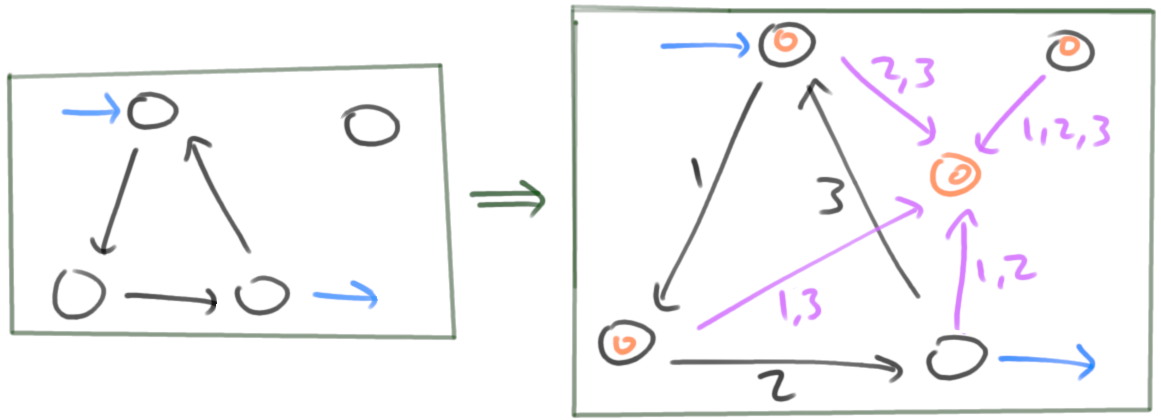
\includegraphics[width=10cm]{ALL_DFA_in_NL.png}
	\end{center}
	We will show that \(\textit{ALL}_{\textsf{DFA}}\) by proving \(\ol{\textit{PATH}} \logredu \textit{ALL}_{\textsf{DFA}}\). Suppose we have some instance \(\angles{G, s, t}\) of \(\textit{PATH}\) where \(G = (V, E)\). Consider the \textsf{DFA} \(M\) where the states are \(V \union q_A\) where \(q_A\) is a new accepting state. Moreover, everything except \(t\) is an accepting state. Label each each transition with its own symbol. Then, in order to make it a \textsf{DFA}, all of the remaining edges will go to \(q_A\).

	If \(\angles{G, s, t} \in \ol{\textit{PATH}}\), then there is no way to get to the reject state, and \(M \in \textit{ALL}_{\mathsf{DFA}}\). Conversely, if \(\angles{G, s, t} \in \textit{PATH}\), there exists some sequence of edges (and therefore indices) that reach the non-accepting state, and \(M \notin \textit{ALL}_{\mathsf{DFA}}\).
\end{proof}





% the braces means that we'll do it if we have time, which means we won't do it


\end{document}


% \documentclass{scrartcl}
\usepackage{chez}

\begin{document}
%\chapter{November 19, 2019}
\section{Hierarchy Theorems}
So far, we have that
\[
  \mathsf{L} \subseteq
  \mathsf{NL} \subseteq
  \mathsf{P} \subseteq
  \mathsf{NP} \subseteq
  \mathsf{PSPACE} = \mathsf{NPSPACE}.
\]
Today we will show that \(\mathsf{NL} \subsetneq \mathsf{PSPACE}\). First, we will work with space as it is slightly easier, and then prove similar results for time.

\subsection{Space}
\begin{definition}
  A function \(f \colon \NN \to \NN\), where \(f(n) = O(\log n)\) is \vocab{space constructible} if \(\mathtt 1^n \mapsto f(n)\) is computable in \(O(f(n))\) space.
\end{definition}
\begin{example}
  Most functions like \(\log n\) or \(\exp n\) are space constructible. However, \(f(n) = \log \log \log n\) is not space constructible. In particular, if a \textsf{TM} runs in \(O(\log \log \log n)\) space, then it can only recognize a regular language, which is basically having no tape. This implies that any \textsf{TM} that has a space complexity less than \(O(\log \log \log n)\) can only recognize a regular language. This space is called a \vocab{gap}.
\end{example}


\begin{theorem}[Space hierarchy theorem]<space_hierarchy>
  If \(f \colon \NN \to \NN\) is space constructible, there exists a language \(A\) decidable in \(O(f(n))\) space but not \(o(f(n))\) space.
\end{theorem}
\begin{proof}
  The idea is to find a machine \(D\) that runs in space \(O(f(n))\) and such that \(L(D) \neq L(M)\) for all \(M\) running in \(o(f(n))\) space. We can easily force \(D\) to run in \(O(f(n))\) space by just using \(f(n)\) space. To ensure that \(L(D)\) is not decidable in \(o(f(n))\) space, we will use the idea from diagonalization. In particular, If \(M\) is a machine potentially deciding \(L(D)\) in \(o(f(n))\) space, we will make \(M\) and \(D\) disagree on \(\angles M\).
  
  Consider the following machine:
  \begin{enumerate}[start=0]
    \item On input \(w\):
    \item Let \(n \gets \size w\).
    \item Since \(f\) is space constructible, compute \(f(n)\) and mark off this much tape. If the later steps try to use more then \textsc{reject}.
    \item If \(w\) is not of the form \(\angles M \mathtt 1 \mathtt 0^n\) for some \textsf{TM} \(M\), then \textsc{reject}.
    \item Simulate \(M\) on \(w\) for \(2^{f(n)}\) steps. If it reaches this point, \textsc{reject}.
    \item If \(M\) accepts, then \textsc{reject}. If \(M\) rejects, then \textsc{accept}.
  \end{enumerate}

  The reason why we only run \(M\) for \(2^{f(n)}\) is because we don't want it loop. We arbitrarily choose to reject if \(M\) loops (because \(M\) is not a decider anyway).

  Now suppose that \(M\) runs in \(o(f(n))\) space. Then consider running the machine on \(\angles M\). The algorithm will not reject in steps 3 or 4, and in step 5, it will do the opposite of what \(M\) on \(\angles M\) does. Therefore, \(M\) cannot decide the language of this machine.
\end{proof}

\begin{corollary}
  \(\mathsf{NL} \subsetneq \mathsf{PSPACE}\).
\end{corollary}
\begin{proof}
  By Savitch's theorem, \(\mathsf{NL} \subseteq \SPACE((\log n)^2)\). By the space hierarchy theorem, \(\SPACE((\log n)^2) \subsetneq \SPACE(n) \subseteq \mathsf{PSPACE}\). Therefore, \(\mathsf{NL} \subsetneq \mathsf{PSPACE}\).
\end{proof}


\subsection{Time}
Our results for time will be very similar to space.

\begin{definition}
  A function \(t \colon \NN \to \NN\) is \vocab{time constructible} if \(\mathtt 1^n \mapsto t(n)\) is computable in \(O(t(n))\) time.
\end{definition}

\begin{theorem}[Time hierarchy theorem]
  If \(t\colon \NN \to \NN\) is time constructible, then there exists a language \(A\) decidable in \(O(t(n))\) time but not \(o(t(n)/\log n)\) time.
\end{theorem}

The reason why we have an extra factor of \(\log n\) is because in order to use the same proof, we must keep a counter of the number of steps used near the head. It is possible for a stronger theorem to be true, but we cannot use the same proof as we did in space.

\begin{proof}
  The proof is very similar to the proof for \cref{thm:space_hierarchy}. Let \(D\) be the machine:
  \begin{enumerate}[start=0]
    \item On input \(w\):
    \item Let \(n \gets \size w\).
    \item Since \(t\) is space constructible, compute \(t(n)\) and make a binary counter with the value \(\ceil{t(n) / \log t(n)}\).
    \item If \(w\) is not of the form \(\angles M \mathtt 1 \mathtt 0^n\) for some \textsf{TM} \(M\), then \textsc{reject}.
    \item Simulate \(M\) on \(w\) for \(\ceil{t(n) / \log t(n)}\) steps using the counter, and moving the counter with the head.
    \item If \(M\) accepts, then \textsc{reject}. If \(M\) rejects, then \textsc{accept}.
  \end{enumerate}

  The factor of \(\log t(n)\) comes from the binary counter and moving it to the head at every step that we're simulating \(M\). Otherwise, everything else is the same.
\end{proof}





\end{document}


% \documentclass{standalone}
\usepackage{chez}

\begin{document}
%\chapter{November 21, 2019}
\section{Intractable Problems}
Recall that we have
\[
	\mathsf{L} \subseteq
	\mathsf{NL} \subseteq
	\mathsf{P} \subseteq
	\mathsf{NP} \subseteq
	\mathsf{PSPACE},
\]
where \(\mathsf{NL} \neq \mathsf{PSPACE}\). The problems of whether \(\mathsf{L} \overset{?}{=} \mathsf{P}\) and \(\mathsf{P} \overset{?}{=} \mathsf{PSPACE}\) are open, but \(\mathsf{NL} \neq \mathsf{PSPACE}\) implies that at least one of them is false.

Recall that \(\textit{EQ}_{\textsf{DFA}}\) is decidable, and using the same \textsf{TM}, we have that \(\textit{EQ}_{\textsf{DFA}} \in \mathsf{P}\). We can also show that \(\textit{EQ}_{\textsf{NFA}} \in \mathsf{PSPACE}\).

\begin{proposition}
	\(\textit{EQ}_{\textsf{NFA}} \in \mathsf{PSPACE}\).
\end{proposition}
\begin{proof}
	Since \(\mathsf{PSPACE}\) is deterministic, \(A \in \mathsf{PSPACE} \iff \ol A \in \mathsf{PSPACE}\). We proceed by showing that \(\ol{\textit{EQ}_{\mathsf{NFA}}} \in \mathsf{NPSPACE = \mathsf{PSPACE}}\). The idea is to nondeterministically guess the string that yields different results for the two \textsf{NFA}s. It is clear that this runs in polynomial space.
\end{proof}

Similarly, we have a similar theorem for regular expressions:
\begin{corollary}
	\(\textit{EQ}_{\textsf{REGEX}} \in \mathsf{PSPACE}\).
\end{corollary}
\begin{proof}
	This is immediately because the conversion from \(\textsf{REGEX} \to \textsf{NFA}\) can be done in polynomial space.
\end{proof}


\subsection{Exponential Space}
Consider a modified version of regular expressions that has exponentiation, i.e.
\[
	R^i = \underbracket{RR \dots R}_{\text{$i$ times}}.
\]
Let a regular expression with this feature be called an \(\REGEXup\).

\begin{definition}
	Let the languages decidable in exponential time and space be, respectively
	\begin{gather*}
		\mathsf{EXPTIME} = \bigunion_k \TIME(2^{n^k}) \\
		\mathsf{EXPSPACE} = \bigunion_k \SPACE(2^{n^k}).
	\end{gather*}
\end{definition}

\begin{definition}
	We say that a language \(B\) is \vocab{\(\mathsf{EXPSPACE}\)-complete} if
	\begin{itemize}
		\item \(B \in \mathsf{EXPSPACE}\) and
		\item for all \(A \in \mathsf{EXPSPACE}\), we have \(A \polyredu B\), i.e. is \vocab{\(\mathsf{EXPSPACE}\)-hard}.
	\end{itemize}
\end{definition}

\begin{theorem}
	\(\textit{EQ}_{\REGEXup} = \set{\angles{R_1, R_2} \mid \text{%
		$R_1$ and $R_2$ are $\REGEXup$ such that $L(R_1) = L(R_2)$%
	}}\) is \(\mathsf{EXPSPACE}\)-complete.
\end{theorem}
\begin{proof}
	We will show that \(\textit{EQ}_{\REGEXup}\) is \(\mathsf{EXPSPACE}\)-complete. It is clear that \(\textit{EQ}_{\REGEXup} \in \mathsf{EXPSPACE}\) because \(\textit{EQ}_{\textsf{REGEX}} \in \mathsf{PSPACE}\). In particular, we can expand the \(\REGEXup\) into a \textsf{REGEX} in exponential space, and then use the \(\mathsf{PSPACE}\) algorithm for \(\textit{EQ}_{\textsf{REGEX}}\) on the exponentially sized \textsf{REGEX}s.

	Now consider some \(A \in \mathsf{EXPSPACE}\) decided by a \textsf{TM} \(M\) that runs in space \(O(2^{n^k})\). Consider the reduction mapping \(w \mapsto \angles{R_1, R_2}\) where \(R_1\) is a \(\REGEXup\) that generates all strings, and \(R_2\) is a \(\REGEXup\) that generates all strings except for the rejecting computation history of \(M\) on \(w\). Then \(M\) accepts \(w\) iff \(L(R_1) = L(R_2)\), as desired.

	To actually construct \(R_2\), we can just check to make sure that the computation history makes a mistake. Let \(\Delta = \Gamma \union Q \union \set{\texttt{\#}}\) be the alphabet for the configurations.
	Consider the configuration history
	\[
		c_1 \texttt{\#} c_2 \texttt{\#} \dots \texttt{\#} c_{\text{reg}},
	\]
	where we pad all configurations at the end with \(\blank\) for convenience. Then let
	\[
		R_2 = R_{\text{bad-start}} \union R_{\text{bad-move}} \union R_{\text{bad-reject}},
	\]
	where the parts are defined as follows (where we adopt the notation \(X - a \coloneqq X \setminus \set{a}\)):
	\begin{itemize}
		\item Let \(R_{\text{bad-start}} = S_0 \union S_1 \union S_2 \union S_n \union S_{\text{blanks}},\) where \(S_i\) means that the \(i\)th character is incorrect. In particular,
		\[
			S_i = \Delta^i (\Delta - w_i) \Delta^*
				\qquad \text{and} \qquad
				S_{\text{blanks}} = \Delta^{n + 1} (\Delta - \eps)^{2^{n^k} - n - 2} (\Delta - \blank) \Delta^*.
		\]
		Note that we have used the exponentiation function of the \(\REGEXup\) so that \(R_{\text{bad-start}}\) is not exponentially long.

		\item Similarly, let \(R_{\text{bad-reject}} = (\Delta - q_{\text{reject}})^*\).

		\item For \(R_{\text{bad-move}}\), we can use the same idea as we did in Cook-Levin. We look at three consecutive symbols in a configuration as well as the configuration after it, and we reject the sets of symbols that do not correspond to a legal move. In particular,
		\[
			R_{\text{bad-move}} = \bigunion_{\text{bad $(abc, def)$}} \Delta^* abc \Delta^{2^{n^k} - 2} def \Delta^*.
		\]
	\end{itemize}

	Note that \(R_2\) is polynomial in length, as desired.
\end{proof}






\end{document}


% \documentclass{standalone}
\usepackage{chez}

\begin{document}
%\chapter{November 26, 2019}

\section{Oracles}
\begin{definition}
  Given a language \(A\), an \vocab{\(A\)-oracle machine} (\(A\)-\textsf{OM}) is a \textsf{TM} that magically knows the answer to \(A\).
\end{definition}
One way to formalize this is to add two extra tapes to our regular \textsf{TM}s. One request tape and one answer tape. When we change the request tape, the answer tape changes to the answer of the instance on the request tape immediately, and we can then read from it.

Even though we can never have oracles in real life, we study oracles because if we can show that we can't solve a problem even with an oracle, then we know the problem is really hard.

\begin{definition}
  Let \(\mathsf{P}^{A}\) be the class of languages solvable in polynomial time by an \textit{A}-\textsf{OM}. If \(L \in \mathsf{P}^{A}\), then we say that we can solve \(L\) in polynomial time relative to \textit{SAT}. We can similarly define \(\mathsf{NP}^{A}\).
\end{definition}

\begin{example}
  A \textit{SAT}-\textsf{OM} can solve \textit{SAT}. In particular, we can copy the input into the request tape, and then accept or reject according to the response we get on the answer tape.
\end{example}

Note that this means that
\[
  \mathsf{NP} \subseteq \mathsf{P}^{\textit{SAT}}.
\]
Having an oracle feels like performing reductions, but it is more powerful. In particular, we can request multiple instances of a problem. Moreover, we know that \(\mathsf{P}^{\textit{SAT}} = \mathsf{co}(\mathsf{P}^{\textit{SAT}}) = \mathsf{coP}^{\textit{SAT}}\) because we are working with determinism, so we also have \(\mathsf{NP} \subseteq \mathsf{coP}^{\textit{SAT}} \implies \mathsf{coNP} \subseteq \mathsf{P}^{\textit{SAT}}\).

\begin{example}
  Let \(\textit{MINFORM} = \set{\angles \phi \mid \text{$\phi$ is a minimal formula}}\). We claim \(\textit{MINFORM} \in \mathsf{coNP}^{\textit{SAT}}\).
  \tcblower
  The idea is to nondeterministically guess a shorter formula \(\varphi\), and then use the oracle to check whether they are equivalent by writing the formula \((\phi \Rightarrow \varphi) \land (\varphi \Rightarrow \phi)\).
\end{example}

\subsection{Limits on Diagonalization}
It turns out that the problem of whether \(\mathsf{P}^{\textit{SAT}} \overset{?}{=} \mathsf{NP}^{\textit{SAT}}\) is open. However, we have the following surprising fact:

\begin{proposition}
  \(\mathsf{P}^{\textit{TQBF}} = \mathsf{NP}^{\textit{TQBF}} \subseteq \mathsf{NPSPACE}\).
\end{proposition}
\begin{proof}
  We know that \(\mathsf{P}^{\mathit{TQBF}} \subseteq \mathsf{NP}^{\mathit{TQBF}}\). Since \(\textit{TQBF}\) is \(\textsf{PSPACE}\)-complete, we have \(\textsf{PSPACE} \subseteq \mathsf{P}^{\textit{TQBF}}\). Therefore, we have the chain of inclusions
  \[
    \mathsf{NP}^{\textit{TQBF}} \subseteq
    \mathsf{NPSPACE} = \mathsf{PSPACE} \subseteq \mathsf{P}^{\textit{TQBF}},
  \]
  where the first inclusion is from the fact that \(\textit{TQBF} \in \mathsf{NPSPACE}\), so an \(\mathsf{NPSPACE}\) machine can just solve \textit{TQBF} itself instead of asking the oracle. Therefore, \(\mathsf P^{\textit{TQBF}} = \mathsf{NP}^{\mathit{TQBF}}\).
\end{proof}

Note that if we can use a diagonalization argument to show that \(\mathsf{P} \neq \mathsf{NP}\), then we can just use the same argument to show that \(\mathsf{P}^{\textit{A}} \neq \mathsf{NP}^{\textit{A}}\). However, this is a contradiction for \(A = \textit{TQBF}\), so we cannot use a pure diagonalization argument to prove \(\mathsf{P} \neq \mathsf{NP}\).

\begin{question}
  Recall that \(A_{\textsf{TM}}\) is undecidable from diagonalization. Why doesn't this rule out the existence of \(A_{\textsf{TM}}\)-\textsf{OM}s?
  \tcblower
  Diagonalization only states that \(A_{\textsf{TM}}\) is undecidable by regular \textsf{TM}s, and that \(A_{\textsf{$L$-OM}}\) is undecidable by \(L\)-\textsf{OM}s.
\end{question}



\subsection{More Oracle Problems}
Suppose we have two friends (but not that good of friends that they trust each other) Al and Bo (short for Alice and Bob) that want to split cake fairly.

The protocol goes as follows. There is a cake and several predetermined cuts. Al selects a subset of the cuts, and the cake is cut along those curves. If this process produces \(n\) pieces of cake, Bo then selects \(\ceil{n/2}\) pieces.

\begin{example}
  If this was the original cake with predetermined cuts, Al can select all the cuts, and Bo must select two pieces, guaranteed to have equal area, so Al can guarantee fair cuts.

  \begin{center}
    \begin{tikzpicture}[scale=0.7]
      \draw (0, 0) -- +(0: 4) -- +(60: 4) -- cycle;
      \draw[dashed, cyan] (2, 0) -- +(60: 2) -- +(120: 2) -- cycle;
    \end{tikzpicture}
  \end{center}
\end{example}

Let the problem be
\[
  \textit{CAKE} = \set{
    (\text{cakes}, \text{allowed cuts}) \mid \text{Al can guarantee fair cuts}
  }
\]

\begin{proposition}
  \(\textit{CAKE} \in \mathsf{NP}^{\textit{UNSAT}}\), i.e.\ using an \textsf{NTM} with an \(\textit{UNSAT}\) oracle, we can solve \(\textit{CAKE}\).
\end{proposition}
\begin{proof}
  Consider the following algorithm. Let the \textsf{NTM} nondeterministically select the subset of cuts that Al chooses. We have some pieces of cake with certain volumes. Consider the formula that says ``the volumes of the partition are unequal'', where the variables are indicator variables of whether a piece is in the partition. Then, use the oracle to determine whether this formula is unsatisfiable. If so, then any choice Bo will make must be fair.
\end{proof}

\begin{example}
  Consider the problem
  \[
    \textit{GETSAT} = \set{
      \angles{\phi, i, b} \mid \text{$\phi$ is satisfiable where in the minimal satisfying assignment, the $i$th variable is $b$}
    }.
  \]
  Then \(\textit{GETSAT} \in \mathsf{P}^{\textit{SAT}}\) because we can substitute in \(b\) for the \(i\)th variable of \(\phi\), and then ask the oracle whether the new formula is satisfiable.
\end{example}


\section{Probabilistic Turing Machines}
\begin{definition}
  Let a \vocab{probabilistic Turing machine} (\textsf{PTM}) be a decider \textsf{NTM} where at each nondeterministic step, there are two options, and there is a \(\half\) probability of choose each option.
\end{definition}

For each branch, we can consider the probability that the machine has taken it, i.e.\ \(2^{-k}\), where \(k\) is the number of nondeterministic states in that branch. Then, we define
\[
  \PP[\text{$M$ accepts $w$}] \coloneqq \sum_{\substack{\text{accepting} \\ \mathclap{\text{branches $b$}}}} \PP[\text{$M$ takes branch $b$}],
\]
and \(\PP[\text{$M$ rejects $w$}] \coloneqq 1 - \PP[\text{$M$ accepts $w$}]\).

\begin{definition}
  For some \(\eps > 0\), we say that a \textsf{PTM} \(M\) decides \(A\) with error probability \(\eps\) if:
  \begin{itemize}
    \item for all \(w \in A\), \(\PP[\text{$M$ accepts $w$}] > 1 - \eps\) and
    \item for all \(w \notin A\), \(\PP[\text{$M$ rejects $w$}] > 1 - \eps\).
  \end{itemize}
\end{definition}

Then we can define a new complexity class.
\begin{definition}[Bounded Probabilistic Polynomial Time]
  Let \(\mathsf{BPP} = \set{A \mid \text{some polynomial time \textsf{PTM} decides $A$ with error probability $1/3$}}\).
\end{definition}

The \(\frac{1}{3}\) in the definition seems a bit strange. It turns out that the choice of the constant here does not matter!
\begin{proposition}[Amplification Lemma]
  For \(0 < \eps_1, \eps_2 < \half\), any \textsf{PTM} \(M_1\) with error probability \(\eps_1\) has an equivalent \textsf{PTM} \(M_2\) with error probability \(\eps_2\).
\end{proposition}
\begin{proof}[Sketch]
    \(M_2\) can just run \(M_1\) multiple times, and return the answer that appears the most often.
\end{proof}
Therefore, we have the equivalent definition
\[
  \mathsf{BPP} = \set*{A \mid \text{some polynomial time \textsf{PTM} decides $A$ with error probability $\eps < \half$}}.
\]



\end{document}


% \documentclass{standalone}
\usepackage{chez}

\begin{document}
%\chapter{December 03, 2019}
\section{Branching Programs}

\begin{definition}
	A \vocab{branching program} (\textsf{BP}) is a directed acyclic graph where all nodes are labeled with a variable, and have two outgoing edges labeled \(\mathtt 0\) and \(\mathtt 1\). There are two other output nodes labeled \(\mathtt 0\) and \(\mathtt 1\) that have no outgoing edges. Branching programs generally represent a boolean function, where we query each variable when we get to each node and follow the corresponding edge.
\end{definition}

\begin{example}[Branching program]
	\centering
	\begin{tikzpicture}[automaton]
		\node[state, initial, initial text={}] (x1) {\(x_1\)};
		\node[state, below left=of x1] (x2) {\(x_2\)};
		\node[state, below right=of x1] (x3) {\(x_3\)};
		\node[state, below left=of x2] (x32) {\(x_3\)};
		\node[state, below left=of x3] (x4) {\(x_4\)};
		\node[state, below right=of x3] (x22) {\(x_2\)};
		\node[state, below left=of x4] (out0) {\(\mathtt 0\)};
		\node[state, below right=of x4] (out1) {\(\mathtt 1\)};

		\begin{scope}[inner sep=1pt]
			\draw (x1) edge node{\(\mathtt 0\)} (x2);
			\draw (x1) edge node[swap]{\(\mathtt 1\)} (x3);
			\draw (x2) edge node{\(\mathtt 0\)} (x32);
			\draw (x2) edge node[swap]{\(\mathtt 1\)} (x4);
			\draw (x3) edge node{\(\mathtt 0\)} (x4);
			\draw (x3) edge node[swap]{\(\mathtt 1\)} (x22);

			\draw (x32) edge node[swap]{\(\mathtt 0\)} (out0);
			\draw (x32) edge node[near start]{\(\mathtt 1\)} (out1);

			\draw (x4) edge node[swap, near start]{\(\mathtt 0\)} (out0);
			\draw (x4) edge node[near start]{\(\mathtt 1\)} (out1);

			\draw (x22) edge node[swap, near start]{\(\mathtt 0\)} (out0);
			\draw (x22) edge node{\(\mathtt 1\)} (out1);
		\end{scope}
	\end{tikzpicture}
\end{example}

We call a branching program \vocab{read-once} if every path from the start to one of the output nodes contains each variable at most once. We will abbreviate read-once branching programs as \textsf{ROBP}s. Then consider the problem \(\textit{EQ}_{\textsf{ROBP}}\).

\begin{claim}
	\(\textit{EQ}_{\textsf{ROBP}} \in \mathsf{BPP}\).
\end{claim}
One attempt at proving this is to try the following algorithm:
\begin{enumerate}[start=0]
	\item On input \(\angles{B_1, B_2}\):
	\item Pick random boolean assignments to \(x_1, \dots, x_m\) and run \(B_1, B_2\) on these assignments.
	\item If they disagree then \textsc{reject}, else \textsc{accept}.
\end{enumerate}
It turns out that this does not work because the two branching programs might only disagree on one input, so the algorithm will get that specific instance wrong with probability \(1 - 2^m\).

Instead to prove this, we will need a lemma that follows from the fundamental theorem of algebra.
\begin{lemma}[Schwartz-Zippel Lemma]
	If \(p \in \FF_q[x_1, \dots, x_m]\) is nonzero and has degree at most \(d\) in each variable, then over \(r_1, \dots, r_m \in \FF_q\),
	\[
		\PP[p(x_1, \dots, x_m) = 0] \leq \frac{md}{q}.
	\]
\end{lemma}
\begin{proof}[Sketch]
	Induct on \(m\). Write \(p(x_1, \dots, x_m)\) as a polynomial in \(F[x_1, \dots, x_{m - 1}][x_m]\) and use the fundamental theorem of algebra.
\end{proof}




\end{document}


% \documentclass{scrartcl}
\usepackage{chez}

\begin{document}
Recall that we can label each object (nodes and edges) of a \textsf{BP} with \(\mathtt 1\)s and \(\mathtt 0\)s depending on which ones are used during the execution. We can even do this for general variables and also algebraically.

\begin{example}
  \centering
  \begin{tikzpicture}[automaton]
    \node[state, initial above, initial text={}] (x1) {\(x_1\)};
    \node[state, below left =1.4 and 1.3 of x1] (x2l) {\(x_2\)};
    \node[state, below right=1.4 and 1.3 of x1] (x2r) {\(x_2\)};
    \node[state, below=1.5 of x2l] (out0) {\(\mathtt 0\)};
    \node[state, below=1.5 of x2r] (out1) {\(\mathtt 1\)};

    \begin{scope}[inner sep=1pt]
      \definecolor{markblue}{rgb}{0.2, 0.5, 1}
      \NewDocumentCommand{\marknode}{m}{\scalebox{0.7}{\color{markblue}#1}}
      \path (x1) edge
        node[swap, pos=0.2]{\(\mathtt 0\)}
        node[swap]{\marknode{1}}
        (x2l);
      \path (x1) edge
        node[pos=0.2]{\(\mathtt 1\)}
        node{\marknode{0}}
        (x2r);
      \path (x2l) edge
        node[swap, pos=0.18]{\(\mathtt 0\)}
        node[swap]{\marknode{0}}
        (out0);
      \path (x2l) edge
        node[pos=0.06]{\(\mathtt 1\)}
        node[pos=0.2]{\marknode{1}}
        (out1);
      \path (x2r) edge
        node[swap, pos=0.06]{\(\mathtt 1\)}
        node[swap, pos=0.2]{\marknode{0}}
        (out0);
      \path (x2r) edge
        node[pos=0.18]{\(\mathtt 0\)}
        node{\marknode{0}}
        (out1);

      \node at ([shift={(30:0.4)}]x1){\marknode{1}};
      \node at ([shift={(180:0.4)}]x2l){\marknode{1}};
      \node at ([shift={(0:0.4)}]x2r){\marknode{0}};
      \node at ([shift={(180:0.4)}]out0){\marknode{0}};
      \node at ([shift={(0:0.4)}]out1){\marknode{1}};
    \end{scope}

    \node[right=1.5 of x1] () {\begin{tabular}{c}
        \scriptsize \(x_1 = \mathtt 0\) \\ \scriptsize \(x_2 = \mathtt 1\)
      \end{tabular}};
  \end{tikzpicture}
  \hspace{1.5cm}
  \begin{tikzpicture}[automaton]
    \node[state, initial above, initial text={}] (x1) {\(x_1\)};
    \node[state, below left =1.4 and 1.3 of x1] (x2l) {\(x_2\)};
    \node[state, below right=1.4 and 1.3 of x1] (x2r) {\(x_2\)};
    \node[state, below=1.5 of x2l] (out0) {\(\mathtt 0\)};
    \node[state, below=1.5 of x2r] (out1) {\(\mathtt 1\)};

    \begin{scope}[remember picture]
      \tikzstyle{reverseclip}=[insert path={
        (current bounding box.south west)
        rectangle (current bounding box.north east)}
      ]
      \definecolor{markblue}{rgb}{0.2, 0.5, 1}
      \NewDocumentCommand{\marknode}{m}{\scalebox{0.7}{\color{markblue}#1}}
      \path (x1) edge
        node[swap, pos=0.2]{\(\mathtt 0\)}
        node[swap]{\marknode{\(1 - x_1\)}}
        (x2l);
      \path (x1) edge
        node[pos=0.2]{\(\mathtt 1\)}
        node{\marknode{\(x_1\)}}
        (x2r);
      \path (x2l) edge
        node[swap, pos=0.18]{\(\mathtt 0\)}
        node[swap]{\marknode{\((1 {-} x_1)(1 {-} x_2)\)}}
        (out0);
      \begin{scope}
        \makeatletter
        \tikzset{use path/.code={\pgfsyssoftpath@setcurrentpath{#1}}}
        \makeatother
        \path (x2l) edge[draw=none]
          node[pos=0.06]{\(\mathtt 1\)}
          node[
            inner sep=0.5pt,
            shift={(-0.3, -0.15)},
            pos=0.2,
            save path=\tmpprotect]
          {\marknode{\((1 {-} x_1) x_2\)}}
          (out1);
        \path[clip][use path=\tmpprotect] [reverseclip];
        \path (x2l) edge (out1);
      \end{scope}
      \path (x2r) edge
        node[swap, pos=0.06]{\(\mathtt 1\)}
        node[pos=0.2]{\marknode{\(x_1 x_2\)}}
        (out0);
      \path (x2r) edge
        node[pos=0.18]{\(\mathtt 0\)}
        node{\marknode{0}}
        (out1);

      \node at ([shift={(30:0.4)}]x1){\marknode{\(1\)}};
      \node at ([shift={(180:0.65)}]x2l){\marknode{\(1 {-} x_1\)}};
      \node at ([shift={(0:0.45)}]x2r){\marknode{\(x_1\)}};
      \node at ([shift={(-110:0.45)}]out0){\marknode{\(x_1 x_2 {+} (1 {-} x_1) (1 {-} x_2)\)}};
      \node at ([shift={(-70:0.45)}]out1){\marknode{\(x_1(1 {-} x_2) {+} x_2(1 {-} x_1)\)}};
    \end{scope}
  \end{tikzpicture}
  %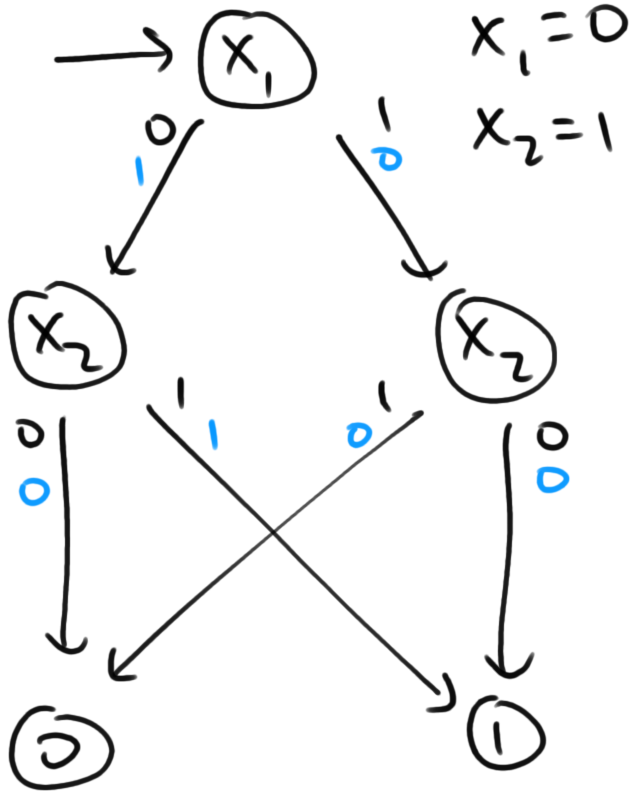
\includegraphics[scale=0.2]{EQ_ROBP_in_BPP1}
  %\qquad
  %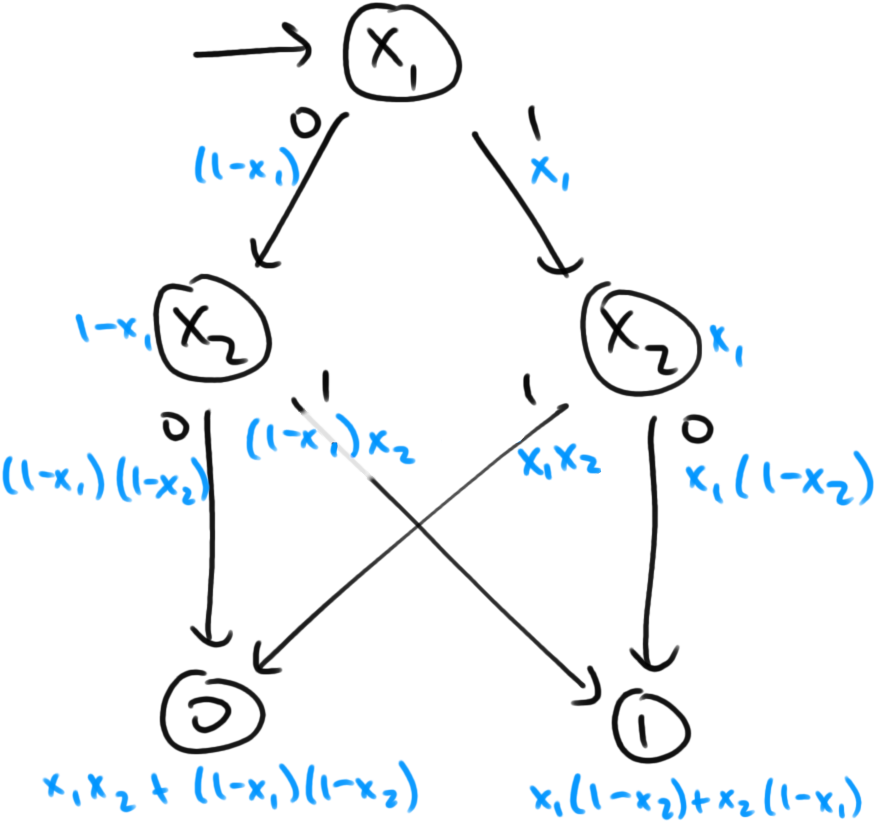
\includegraphics[scale=0.2]{EQ_ROBP_in_BPP2}
\end{example}

More generally, we have the following labeling rules
\begin{center}
  \begin{tikzpicture}[automaton]
    \definecolor{markblue}{rgb}{0.2, 0.5, 1}
    \NewDocumentCommand{\marknode}{m}{\scalebox{0.7}{\color{markblue}#1}}

    \node[state, label=below:{\marknode{\(a + b + c\)}}] (q) {};
    \node[above left=of q] (anode) {};
    \node[above=of q] (bnode) {};
    \node[above right=of q] (cnode) {};

    \path (anode) edge node[swap]{\marknode{\(a\)}} (q);
    \path (bnode) edge node{\marknode{\(b\)}} (q);
    \path (cnode) edge node{\marknode{\(c\)}} (q);
  \end{tikzpicture}
  \qquad
  \begin{tikzpicture}[automaton]
    \definecolor{markblue}{rgb}{0.2, 0.5, 1}
    \NewDocumentCommand{\marknode}{m}{\scalebox{0.7}{\color{markblue}#1}}

    \node[state, label=above:{\marknode{\(a\)}}] (q) {};
    \node[below left=of q] (anode) {};
    \node[below right=of q] (cnode) {};

    \tikzset{inner sep=1pt}
    \path (q) edge node[swap, pos=0.2]{\(\mathtt 0\)} (anode);
    \path (q) edge node[swap, inner sep=1pt, pos=0.5]{\marknode{\(a(1 {-} x_i)\)}} (anode);
    \path (q) edge node[pos=0.2]{\(\mathtt 1\)} (cnode);
    \path (q) edge node[inner sep=1pt, pos=0.5]{\marknode{\(a x_i\)}} (cnode);
  \end{tikzpicture}
  %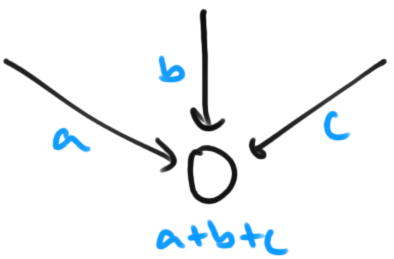
\includegraphics[scale=0.25]{EQ_ROBP_in_BPP3}
  %\qquad
  %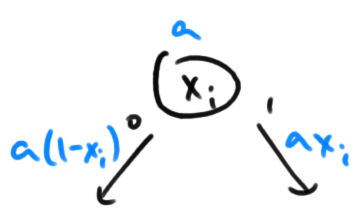
\includegraphics[scale=0.27]{EQ_ROBP_in_BPP4}
\end{center}
Then, the formula the corresponds to the \(\mathtt 1\) output is the one the represents the \textsf{BP}.

\begin{claim}
  For \textsf{ROBP}s \(B_1\) and \(B_2\) with polynomials \(P_1\) and \(P_2\), then over \(r_1, \dots, r_m \in \FF_q\),
  \[
    \PP[P_1(r_1, \dots, r_m) = P_2(r_1, \dots, r_m)] = \begin{cases}
      1 & \text{$B_1$ and $B_2$ are equivalent} \\[-1ex]
      \leq \frac{m}{q} & \text{else}.
    \end{cases}
  \]
\end{claim}
\begin{proof}[Sketch]
  Since \(B_1\) and \(B_2\) are read-once, the degree of
  the polynomials \(P_1\) and \(P_2\) in each variable is at most \(1\).

  Now suppose that \(B_1\) and \(B_2\) are equivalent.
  Note that \(P_1\) and \(P_2\) can be written as sums of
  terms of the form \(y_1 y_2 \dotsm y_m\),
  where \(y_i\) is either \(x_i\) or \(1 - x_i\).
  (If a certain variable \(x_i\) is not on a path,
  we can use the fact that \(1 = x_i + (1 - x_i)\) and expand.)
  Moreover, in this form, the polynomials give us precisely
  the inputs of the \textsf{ROBP}s that output \(1\).
  Therefore, \(P_1\) and \(P_2\) are the same in this case.

  Now suppose that \(B_1\) and \(B_2\) are not equivalent.
  Then note that \(P_1 - P_2 \neq 0\) from looking at
  the representation of \(P_1\) and \(P_2\) with
  terms of the form \(y_1 y_2 \dotsm y_m\) as before.

  The \(\frac{md}{q}\) is from Schwartz-Zippel.
  Since these are read-once \textsf{BP}s, we have \(d = 1\),
  so \(\PP = \frac{m}{q}\).
  We can choose \(q \geq 3m\), so \(\PP \leq \frac{1}{3}\), as desired.
\end{proof}

\begin{corollary}
  \(\textit{EQ}_{\textsf{ROBP}} \in \mathsf{BPP}\).
\end{corollary}


\section{Interactive Proofs}
Consider the problem of graph isomorphism (denoted by \(G_1 \iso G_2\)):
\[
  \textit{ISO} = \set{\angles{G_1, G_2} \mid G_1 \iso G_2}.
\]
It is clear that \(\textit{ISO} \in \mathsf{NP}\) because a certificate
would just be a bijection of the vertices.
However, \textit{ISO} is not known to be
\(\mathsf{NP}\)-hard or in \(\mathsf{P}\).

Suppose that we have two graphs \(G_1\) and \(G_2\).
Also suppose that we have two parties named \(P\) (prover) and \(V\) (verifier).
If \(V\) runs in probabilistic polynomial time,
and \(P\) has unlimited computation power,
then how can \(P\) prove to \(V\) that \(G_1 \iso G_2\) or \(G_1 \ncong G_2\)?

Consider the following protocol:
\begin{enumerate}
  \item \(P\) claims either \(G_1 \iso G_2\) or \(G_1 \not\iso G_2\).
  \item If \(P\) claimed \(G_1 \iso G_2\), then \(P\) provides the certificate,
    and \(V\) checks it.
    \(V\) either \textsc{accepts} or \textsc{rejects} at this case.
  \item If \(P\) claims \(G_1 \not\iso G_2\),
    then \(V\) repeats the following procedure \(N\) times:
  \begin{enumerate}
    \item \(V\) secretly takes one of \(G_1, G_2\) randomly and
      scrambles it to another graph \(G\) isomorphic to the selection.
    \item \(V\) asks \(P\) which of \(G_1\),
      \(G_2\) that \(G\) is isomorphic to.
  \end{enumerate}
  \item If \(P\) gets all of them right,
    then \(V\) \textsc{accepts}, else \textsc{reject}.
\end{enumerate}

Note that if \(P\) lies in the first case,
then \(V\) will know with the certificate.
In the other case, \(V\) will catch the lie with probability \(1 - 2^{-N}\).

\begin{definition}
  Consider two parties \(P\) unlimited computation and
  \(V\) with probabilistic polynomial computation respectively.
  Both exchange messages until \(V\) accepts or rejects. Let
  \[
    \PP[\text{$(V\leftrightarrow P)$ accepts $w$}] \coloneqq
      \PP[\text{$V$ ends up accepting}].
  \]
\end{definition}
\begin{definition}
  Let \(\mathsf{IP}\) (for \vocab{interactive proofs}) be
  \begin{align*}
    \mathsf{IP} \coloneqq \lbrace
      A \mid {}& \text{there exists a protocol $(V \leftrightarrow P)$ where} \\
      {}& w \in A \iff \PP[\text{$(V\leftrightarrow P)$ accepts $w$}] \geq \tfrac{2}{3} \\
      {}& \text{$w \notin A \iff \PP[\text{$(V\leftrightarrow \tilde P)$ accepts $w$}] \leq \tfrac{1}{3}$ for all $\tilde P$}
    \rbrace.
  \end{align*}
\end{definition}

We know that \(\mathsf{NP} \subseteq \mathsf{IP}\) because
the prover can just send the certificate.

We also know that \(\mathsf{BPP} \subseteq \mathsf{IP}\) because
the verifier can tell the prover to go away and just do the problem themself.

It turns out that \(\mathsf{IP} \subseteq \mathsf{PSPACE}\),
but we will not prove this. The idea of the proof is to
explore all possible interactions in polynomial space.
We will prove the weaker statement \(\mathsf{coNP} \subseteq \mathsf{IP}\)
by showing \(\texttt\#\mathit{SAT} \in \mathsf{IP}\).
(Note that \(\texttt\#\mathit{SAT}\) is \(\mathsf{coNP}\)-hard
  because \(\overline{\mathit{SAT}} \polyredu \texttt\#\mathsf{SAT}\)
  by the reduction \(\angles{\phi} \to \angles{\phi, 0}\).)


\end{document}

% \documentclass{standalone}
\usepackage{chez}

\begin{document}
%\chapter{December 10, 2019}
\section{\texorpdfstring{\(\texttt\#\textit{SAT} \in \mathsf{IP}\)}{\#SAT in IP}}
Consider the problem
\[
  \textsf\#\textit{SAT} = \set{
    \angles{\phi, k} \mid \text{$\phi$ has exactly $k$ satisfying assignments}
  }.
\]
For a formula \(\phi\) on variables \(x_1, \dots, x_m\) and
\(a_1, \dots, a_i \in \set{\mathtt 0, \mathtt 1}\),
let \(\numphi(a_1, \dots, a_i)\) be the number of satisfying assignments
with presets \(x_1 = a_1\), \(x_2 = a_2\), \ldots, \(x_i = a_i\).
Then,
\begin{itemize}
  \item \(\numphi(a_1, \dots, a_i) = \numphi(a_1, \dots, a_i, \mathtt 0) +
                                     \numphi(a_1, \dots, a_i, \mathtt 1)\), and
  \item \(\numphi(a_1, \dots, a_m) = \phi(a_1, \dots, a_m)\).
\end{itemize}

There is a straightforward exponential protocol for \(\texttt\#\textit{SAT}\).
Suppose that \(P\) claims that \(\angles{\phi, k} \in \texttt\#\textit{SAT}\).
\begin{enumerate}[start=0]
  \item \(P\) sends \(\numphi()\), and \(V\) checks \(k = \numphi()\).
  \item \(P\) sends \(\numphi(\mathtt 0), \numphi(\mathtt 1)\),
    and \(V\) checks \(\numphi() = \numphi(\mathtt 0) + \numphi(\mathtt 1)\).
  \item \(P\) sends \(\numphi(\mathtt{00}),
                      \numphi(\mathtt{01}),
                      \numphi(\mathtt{10}),
                      \numphi(\mathtt{11})\),
    and \(V\) checks \(\numphi(\mathtt 0) = \numphi(\mathtt{00}) +
                                            \numphi(\mathtt{01})\)
                 and \(\numphi(\mathtt 1) = \numphi(\mathtt{10}) +
                                            \numphi(\mathtt{11})\).
  \item[\(\vdots\)]
  \item[\(m\).] \(P\) sends \(\numphi(\mathtt{0}^m), \dots,
                              \numphi(\mathtt 1^m)\), and \(V\) checks
    \(\numphi(\mathtt 0^{m - 1}) = \numphi(\mathtt 0^m) +
                                   \numphi(\mathtt 0^{m - 1} \mathtt 1), \dots,
      \numphi(\mathtt 1^{m - 1}) = \numphi(\mathtt 1^{m - 1} \mathtt 0) +
                                   \numphi(\mathtt 1^m)\).
  \item[\(m + 1\).] \(V\) checks \(\numphi(\mathtt 0^m) = \phi(\mathtt 0^m),
                            \dots, \numphi(\mathtt 1^m) \phi(\mathtt 1^m)\).
\end{enumerate}

The problem is that at every step, we are doubling the number of things that
the prover is sending, because we have to extend the preset variables
by both \(\mathtt 0\) and \(\mathtt 1\).
To fix this, the key idea is to extend by a non-boolean value instead.
We will use the standard arithmetization:
\begin{itemize}[nosep]
  \item \(x \land y \to xy\)
  \item \(\ol x \to 1 - x\)
  \item \(x \lor y \to x + y - xy\)
  \item \(\phi \to \text{some polynomial $P_\phi$ with degree
    less than $\size \phi$}\)
\end{itemize}
Moreover, we can extend \(\numphi\) to be
\[
  \numphi(a_1, \dots, a_i) =
    \sum_{\mathclap{a_{i + 1}, \dots, a_{m} \in \set{\mathtt 0, \mathtt 1}}}
      P_\phi(a_1, \dots, a_i, a_{i + 1}, \dots, a_{m})
\]
over \(a_1, \dots, a_i \in \FF_q\).
Note that we still have
\begin{itemize}
  \item \(\numphi(a_1, \dots, a_i) = \numphi(a_1, \dots, a_i, \mathtt 0) +
                                     \numphi(a_1, \dots, a_i, \mathtt 1)\), and
  \item \(\numphi(a_1, \dots, a_m) = \phi(a_1, \dots, a_m)\).
\end{itemize}
Now consider the new protocol:
\begin{enumerate}[start=0, nosep]
  \item \(P\) sends \(\numphi()\) and \(V\) checks \(k = \numphi()\).

  \item \begin{enumerate}
    \item \(P\) sends \(\numphi(z)\) as a polynomial and
          \(V\) checks \(\numphi() = \numphi(\texttt 0) + \numphi(\texttt 1)\).
          \(V\) can get \(\numphi(\mathtt 0)\) and \(\numphi(\mathtt 1)\)
          by plugging into \(\numphi(z)\).

    \item \(V\) requests a random \(r_1 \in \FF_q\) and
          \(P\) sends \(\numphi(r_1)\).
  \end{enumerate}

  \item \begin{enumerate}
    \item \(P\) sends \(\numphi(r_1, z)\) and
          \(V\) checks \(\numphi(r_1) = \numphi(r_1, \texttt 0) +
                                        \numphi(r_1, \texttt 1)\).

    \item \(V\) requests a random \(r_2 \in \FF_q\) and
          \(P\) sends \(\numphi(r_1, r_2)\).
  \end{enumerate}

  \item[\(\vdots\)]

  \item[\(m\).] \begin{enumerate}
    \item \(P\) sends \(\numphi(r_1, \dots, r_{m - 1}, z)\) and
          \(V\) checks \(\numphi(r_1, \dots, r_{m - 1}) =
                \numphi(r_1, \dots, r_{m - 1}, \texttt 0) +
                \numphi(r_1, \dots, r_{m - 1}, \texttt 1)\).

    \item \(V\) requests a random \(r_m \in \FF_q\) and
          \(P\) sends \(\numphi(r_1, \dots, r_m)\).
  \end{enumerate}

  \item[\(m + 1\).] \(V\) checks
                    \(\numphi(r_1, \dots, r_m) = P_{\phi(r_1, \dots, r_m)}\)
                    and \textsc{accept}s if true.
\end{enumerate}




\end{document}


% insert here


%\documentclass{scrartcl}
\usepackage{chez}

\begin{document}
\chapter{Important things for the exam maybe}
\begin{itemize}
	\item \(\mathsf{REG} \subsetneq \mathsf{CFL} \subsetneq \mathsf{P} \subseteq \mathsf{NP} \subseteq \mathsf{IP} = \mathsf{PSPACE} = \mathsf{NPSPACE} \subseteq \mathsf{EXP} \subseteq \mathsf{EXPSPACE} \subsetneq \mathsf{Decid}\)
	\item \(\mathsf{REG} \subsetneq \mathsf{L} \subseteq \mathsf{NL} = \mathsf{coNL} \subseteq \mathsf{L}^2 \subsetneq \mathsf{PSPACE}\)
	\item \(\mathsf{NL} \subseteq \mathsf{P} \subseteq \mathsf{NP} \intersect \mathsf{coNP}\)
	\item \(\mathsf{coNP} \subseteq \mathsf{PSPACE}\)
	\item \(\mathsf{P} \subsetneq \mathsf{EXP}\)
	\item \(\mathsf{PSPACE} = \mathsf{NPSPACE} \subsetneq \mathsf{EXPSPACE}\)
	\item \(\mathsf{P} \subseteq \mathsf{BPP} \subseteq \mathsf{PSPACE}\)
	\item \(\set{\text{regular languages}} \subseteq \TIME(n)\)
	\item \(\set{\text{context-free languages}} \subseteq \TIME(n^5)\)
	\item \(\mathsf{NL} = \mathsf{coNL}\)
	\item Deterministic classes are closed under complement (e.g. \(\mathsf{P} = \mathsf{coP}\))
	\item Prototypical examples of \(A\)-complete problems:
	\begin{itemize}[nosep]
		\item \(\mathsf{NP}\)-complete \(\textit{SAT}, \textit{$k$-SAT}, \textit{CLIQUE}, \textit{HAMPATH}\)
		\item \(\mathsf{PSPACE}\)-complete \(\textit{TQBF}, \textit{GG}\)
		\item \(\mathsf{NL}\)-complete \(\textit{PATH}, \ol{\textit{PATH}}\)
		\item \(\mathsf{EXPSPACE}\)-complete \(\textit{EQ}_{\REGEXup}\)
	\end{itemize}
	\item \(\mathsf{NP} \subseteq \mathsf{P}^{\textit{SAT}}\)
	\item \(\mathsf{P}^{\textit{SAT}} \subseteq \mathsf{NP}\) is open
	\item \(\mathsf{NP} = \mathsf{coNP}\) is open
	\item \(\mathsf{L} = \mathsf{NL}\) is open
	\item Closure properties
	\begin{center}
		\begin{tabular}{c c c c c c c c} \toprule
			Class (\(X, Y\)) & \(\ol{X}\) & \(X^*\) & \(X^{\mathcal R}\) & \(X \union Y\) & \(X \intersect Y\) & \(X \circ Y\) & \(X \setminus Y\) \\ \midrule
			\(\mathsf{L}\) & Y & ?\footnote{Only if \(\mathsf{L} = \mathsf{NL}\)} & Y & Y & Y & Y & Y \\
			\(\mathsf{NL} = \mathsf{coNL}\) & Y & Y & Y & Y & Y & Y & Y \\
			\(\mathsf{P}\) & Y & Y & Y & Y & Y & Y & Y \\
			\(\mathsf{NP}\) & ? & Y & Y & Y & Y & Y & ? \\
			\(\mathsf{coNP}\) & ? & Y & Y & Y & Y & Y & ? \\
			\(\mathsf{BPP}\) & Y & Y & Y & Y & Y & Y & Y \\
			\(\mathsf{IP} = \mathsf{PSPACE} = \mathsf{NPSPACE}\) & Y & Y & Y & Y & Y & Y & Y \\
			\(\mathsf{EXP}\) & Y & Y & Y & Y & Y & Y & Y \\
			\(\mathsf{EXPSPACE}\) & Y & Y & Y & Y & Y & Y & Y \\ \bottomrule
		\end{tabular}
	\end{center}
	\item \(\textit{ISO}\) is open
	\item Converting a regex to an \textsf{NFA} is in \(L\).
	\item Characterization of \(EQ\) problems
	\begin{itemize}
		\item \(A_{\textsf{DFA}} \in \mathsf{L}\)
	\end{itemize}
	\item Characterization of \(A\) problems
	\begin{itemize}
		\item \(A_{\textsf{DFA}} \in \mathsf{L}\)
	\end{itemize}
\end{itemize}

\end{document}




\end{document}
